\RequirePackage[2020-02-02]{latexrelease}
\documentclass[conference]{IEEEtran}
\IEEEoverridecommandlockouts
% The preceding line is only needed to identify funding in the first footnote. If that is unneeded, please comment it out.

\usepackage{xcolor}
\usepackage[hang, flushmargin]{footmisc}
\usepackage[
colorlinks=false, % don't highlight links in color
linkbordercolor=green, % set border color for internal links
citebordercolor=green, % set border color for citations
filebordercolor=magenta, % set border color for file links
urlbordercolor=cyan, % set border color for URLs
pdfborder={0 0 1}, % determine border around links
linkcolor=black,
citecolor=black,
filecolor=black,
urlcolor=black,
]{hyperref}
\usepackage{footnotebackref}

\usepackage{cite}
\usepackage{amsmath,amssymb,amsfonts}
\usepackage{algorithmic}
\usepackage{graphicx}
\usepackage{textcomp}

\def\BibTeX{{\rm B\kern-.05em{\sc i\kern-.025em b}\kern-.08em
    T\kern-.1667em\lower.7ex\hbox{E}\kern-.125emX}}

\usepackage[english]{babel}
\addto\extrasenglish{  
    \def\figureautorefname{Figure}
    \def\tableautorefname{Table}
    \def\algorithmautorefname{Algorithm}
    \def\sectionautorefname{Section}
    \def\subsectionautorefname{Subsection}
}

\newcommand{\supertiny}{\fontsize{1}{2}\selectfont}

\usepackage{catoptions}
\makeatletter

\def\Autoref#1{%
  \begingroup
  \edef\reserved@a{\cpttrimspaces{#1}}%
  \ifcsndefTF{r@#1}{%
    \xaftercsname{\expandafter\testreftype\@fourthoffive}
      {r@\reserved@a}.\\{#1}%
  }{%
    \ref{#1}%
  }%
  \endgroup
}
\def\testreftype#1.#2\\#3{%
  \ifcsndefTF{#1autorefname}{%
    \def\reserved@a##1##2\@nil{%
      \uppercase{\def\ref@name{##1}}%
      \csn@edef{#1autorefname}{\ref@name##2}%
      \autoref{#3}%
    }%
    \reserved@a#1\@nil
  }{%
    \autoref{#3}%
  }%
}
\makeatother

\usepackage[T1]{fontenc}
\usepackage{graphicx}
%\usepackage{color}
%\renewcommand\UrlFont{\color{blue}\rmfamily}

\usepackage{amsmath,amssymb,amsfonts}
\usepackage[inline, shortlabels]{enumitem}
\usepackage{tabularx}
\usepackage{caption}
\usepackage{listings}
% \usepackage{titlesec}
\usepackage{ragged2e}

\usepackage{xurl}
% \usepackage[hyphens]{url}
\usepackage{pifont}
\usepackage{multirow}
\usepackage[linesnumbered,ruled,vlined]{algorithm2e}
\usepackage{float}
\usepackage{listings}
\usepackage{xcolor}

\definecolor{codegreen}{rgb}{0,0.6,0}
\definecolor{codegray}{rgb}{0.5,0.5,0.5}
\definecolor{codepurple}{rgb}{0.58,0,0.82}
\definecolor{backcolour}{rgb}{0.95,0.95,0.92}
 
\lstdefinestyle{mystyle}{
    backgroundcolor=\color{backcolour},   
    commentstyle=\color{codegreen},
    keywordstyle=\color{magenta},
    numberstyle=\tiny\color{codegray},
    stringstyle=\color{codepurple},
    basicstyle=\footnotesize,
    breakatwhitespace=false,         
    breaklines=true,                 
    captionpos=b,                    
    keepspaces=true,                 
    numbers=left,                    
    numbersep=5pt,                  
    showspaces=false,                
    showstringspaces=false,
    showtabs=false,                  
    tabsize=2
}
 
\lstset{style=mystyle}

% --- Tickz
\usepackage{physics}
\usepackage{amsmath}
\usepackage{tikz}
\usepackage{mathdots}
\usepackage{yhmath}
\usepackage{cancel}
\usepackage{color}
\usepackage{siunitx}
\usepackage{array}
\usepackage{multirow}
\usepackage{amssymb}
\usepackage{gensymb}
\usepackage{tabularx}
\usepackage{extarrows}
\usepackage{booktabs}
\usetikzlibrary{fadings}
\usetikzlibrary{patterns}
\usetikzlibrary{shadows.blur}
\usetikzlibrary{shapes}

% ---------
% \usepackage{titlesec}
\usepackage{pdfpages}
\usepackage{booktabs}
\usepackage{csquotes}
\usepackage{lipsum}  
\usepackage{arydshln}
\usepackage{smartdiagram}
\usepackage{textcomp}
\usepackage{tabularray}\UseTblrLibrary{varwidth}
\usepackage{xcolor}
\def\BibTeX{{\rm B\kern-.05em{\sc i\kern-.025em b}\kern-.08em
    T\kern-.1667em\lower.7ex\hbox{E}\kern-.125emX}}
\usepackage{cite}
\usepackage{amsmath}
\newcommand{\probP}{\text{I\kern-0.15em P}}
\usepackage{etoolbox}
\patchcmd{\thebibliography}{\section*{\refname}}{}{}{}

\setlength\tabcolsep{0.5pt}

\newcommand{\before}[1]{\textcolor{red}{#1}}
\newcommand{\after}[1]{\textcolor{green}{#1}}

\newcommand{\old}[1]{\textcolor{orange}{#1}}
\newcommand{\rem}[1]{\textcolor{red}{#1}}
\newcommand{\todo}[1]{\textcolor{orange}{\newline \textit{\textbf{TODO:} #1}} \newline \newline }



\newcounter{relation}
\setcounter{relation}{0}
\renewcommand{\therelation}{\arabic{relation}}
\newcommand{\relationautorefname}{Relation}

\newenvironment{relation}[1][]{%
    \refstepcounter{relation}%
    \noindent \raggedright \textit{\textbf{Relation. \therelation}} \hfill$}
{%
$ \hfill \phantom{x}

}

\makeatletter
\newcommand{\linebreakand}{%
  \end{@IEEEauthorhalign}
  \hfill\mbox{}\par
  \mbox{}\hfill\begin{@IEEEauthorhalign}
}
\makeatother

% =======================================

\begin{document}

\title{An Organization-oriented MARL Approach for a Cyberdefense Scenario in Drone Swarm}

\author{

    \IEEEauthorblockN{Julien Soulé}
    \IEEEauthorblockA{\textit{Thales Land and Air Systems, BU IAS}}
    %Rennes, France \\
    \IEEEauthorblockA{\textit{Univ. Grenoble Alpes,} \\
        \textit{Grenoble INP, LCIS, 26000,}\\
        Valence, France \\
        julien.soule@lcis.grenoble-inp.fr}

    \and

    \IEEEauthorblockN{Louis-Marie Traonouez}
    \IEEEauthorblockA{\textit{Thales Land and Air Systems, BU IAS} \\
        Rennes, France \\
        louis-marie.traonouez@thalesgroup.com}

    % }

    % \and

    \linebreakand

    \hspace{1.8cm}
    \IEEEauthorblockN{Paul Théron}
    \IEEEauthorblockA{
        \hspace{1.8cm}
        \textit{AICA IWG} \\
        \hspace{1.8cm}
        La Guillermie, France \\
        %lieu-dit Le Bourg, France \\
        \hspace{1.8cm}
        paul.theron@orange.fr}

    \and

    \hspace{0.3cm}
    \IEEEauthorblockN{Jean-Paul Jamont\IEEEauthorrefmark{1}, Michel Occello\IEEEauthorrefmark{2}}
    \IEEEauthorblockA{
        \hspace{0.3cm}
        \textit{Univ. Grenoble Alpes,} \\
        \hspace{0.3cm}
        \textit{Grenoble INP, LCIS, 26000,}\\
        \hspace{0.3cm}
        Valence, France \\
        \hspace{0.3cm}
        \{\IEEEauthorrefmark{1}jean-paul.jamont,\IEEEauthorrefmark{2}michel.occello\}@lcis.grenoble-inp.fr
    }
}

% \IEEEauthorblockN{Michel Occello}
% \IEEEauthorblockA{\textit{Univ. Grenoble Alpes,} \\
% \textit{Grenoble INP, LCIS, 26000,}\\
% Valence, France \\
% michel.occello@lcis.grenoble-inp.fr}


\maketitle

\begin{abstract}
    Autonomous Cyberdefense is increasingly critical for protecting decentralized environments where centralized approaches are impractical. Multi-Agent Reinforcement Learning (MARL) has shown promise in training agents to achieve collective objectives. However, enhancing the monitoring and robustness of MARL in complex environments, such as Cyberdefense scenarios, remains challenging. This paper leverages an algorithmic approach that integrates the $\mathcal{M}OISE^+$ organizational model into the MARL process. Our approach constrains agents' policies according to organizational specifications derived from joint histories, ensuring alignment with predefined roles and missions. We apply our approach to a Cyberdefense scenario involving a drone swarm facing malware attacks. The results demonstrate that our approach effectively guides the training of agents to detect, mitigate, and eliminate malware while adhering to organizational constraints, thereby enhancing the swarm's resilience and operational effectiveness.
\end{abstract}

\begin{IEEEkeywords}
    Multi-Agent Reinforcement Learning, Cyberdefense, Drones, Autonomous Cyber Operation
\end{IEEEkeywords}

% ====================================================================================================

\section{Introduction}
\label{sec:introduction}

\textit{Autonomous Intelligent Cyberdefense Agents}~\cite{Kott2023} (AICA) are agents designed for deployment in networked environments, with primary capabilities including the detection, identification, and characterization of anomalies/attacks, as well as the development and management of countermeasures%
\footnote{
    Theorized by the \textit{AICA International Work Group} (cf. \url{https://www.aica-iwg.org/}) and based on the results of NATO's \textit{Research Task Group IST-152}.
}.
Research into AICA development highlights the increasing need for \textit{Autonomous Cyberdefense} to protect decentralized environments where traditional centralized approaches are ineffective, such as in IoT-based systems. A Multi-Agent System (MAS) offers robust and adaptive defense mechanisms by decomposing the complexity of Cyberdefense into sub-tasks delegated to collaborative agents deployed throughout the system.

The top-down approach involves designing Cyberdefense MAS from predefined architectures and functionalities. The \textit{MAS Centric AICA Reference Architecture} (MASCARA)~\cite{Kott2023} describes AICA-like MAS with components that enable collaborative mechanisms based on explicitly defined plans or processes. However, this approach can be costly as it requires a comprehensive knowledge of the deployment environment, which must be regularly updated due to frequent changes, such as topology modifications or new vulnerabilities.

The bottom-up approach may include Multi-Agent Reinforcement Learning (MARL)~\cite{Albrecht2024}, where agents learn to achieve Cyberdefense goals autonomously, enhancing MAS autonomy~\cite{hammar_stadle4_noms_23}. Despite promising simulation results, this approach lacks the safety guarantees necessary for real-world applications and does not provide explicit means to justify the MAS's success or failure~\cite{dulacarnold2019}. These issues hinder the development of fully or semi-autonomous Cyberdefense MAS, such as AICA, in critical environments, where actions must be justified given their potentially irreversible consequences.

To address these concerns, we propose combining these two point of views by extending \textit{Partial Relation between Agents' History and Organizational Model}~\cite{soule2024} (PRAHOM). PRAHOM is a general approach that leverages histories to integrate $\mathcal{M}OISE^+$ organizational model into the MARL framework. By integrating $\mathcal{M}OISE^+$ organizational specifications into the MARL framework, it has been shown to be possible to constrain learning effectively. However, the current empirical development in this area remains limited and does not scale with the increasing number of organizational specifications. This limitation makes it unsuitable for cyber defense scenarios involving highly complex networked environments.

Partially relying on PRAHOM, we propose a novel algorithm called \textit{PRAHOM Training} (PRAHOMT), which only requires the concepts of role and mission, thus addressing scalability issues. PRAHOMT provides simple means to enhance Cyberdefense MAS performance and ensures safety guarantees by embedding domain-specific knowledge, such as rules, into the training process.

We demonstrate the effectiveness of PRAHOMT through a case study based on the 3rd CAGE Challenge~\cite{cage_challenge_3_announcement}, which involves creating a Cyberdefense MAS for detecting, mitigating, and eliminating malware programs in a drone swarm. We addressed this challenge by creating Cyberdefense MAS models compliant with $\mathcal{M}OISE^+$ formalism, notably inspired by the MASCARA architecture. These models are sets of organizational specifications used by PRAHOMT to guide and constrain agents' training to better achieve the scenario's goals and ensure safety requirements. We verify that the trained agents exhibit expected collective strategies while being fine-tuned throughout the training, making the overall score comparable to leading entries on the leaderboard.

The remainder of this paper is organized as follows. \Autoref{sec:marl_background} presents the basics of MARL relevant to our contribution. \Autoref{sec:related_works} reviews related works considering organizational aspects in MARL. \Autoref{sec:marl_moise_linking} recaps the $\mathcal{M}OISE^+$ organizational model and presents the principles for linking it to MARL. \Autoref{sec:prahom_theory} introduces the PRAHOMT algorithm. \Autoref{sec:experimental_setup} provides an overview of our \textit{Proof of Concept} (PoC) implementation of PRAHOMT and its use for the experimental setup involving MASCARA-based organizational specifications for the 3rd CAGE Challenge. \Autoref{sec:results_and_discussion} discusses the results. Finally, \Autoref{sec:conclusion} concludes the paper and outlines future research directions.

\section{MARL Background}\label{sec:marl_background}

Multi-Agent Reinforcement Learning (MARL) extends the principles of Reinforcement Learning (RL) to scenarios involving multiple interacting agents. Agents aim to maximize the overall cumulative reward through learning, but the presence of other agents introduces additional complexity due to the dynamic nature of the environment.

MARL is often modeled using the Decentralized Partially Observable Markov Decision Process (Dec-POMDP), a framework suitable for environments where agents have limited and differing observations. A Dec-POMDP is formally defined as a tuple $(S, \{A_i\}, T, R, \{\Omega_i\}, O, \gamma)$:

\begin{itemize}
    \item $S$: A finite set of states describing the environment.
    \item $\{A_i\}$: A set of action sets, one for each agent $i$.
    \item $T$: The state transition probability function $T(s, \vec{a}, s') = P(s'|s, \vec{a})$, where $\vec{a}$ is the joint action of all agents.
    \item $R$: The reward function $R(s, \vec{a}, s')$, mapping states and actions to a reward.
    \item $\{\Omega_i\}$: A set of observation sets, one for each agent $i$.
    \item $O$: The observation probability function $O(\vec{o} | s', \vec{a})$, where $\vec{o}$ is the joint observation of all agents.
    \item $\gamma \in [0,1]$: The discount factor for future rewards.
\end{itemize}

In MARL, each agent $i$ maintains a policy $\pi_i: H \times \Omega \rightarrow A$, mapping an action $a \in A$ from an observation $\omega \in \Omega$ and optionally the agent's history $h \in H, h=\langle(\omega_0,a_0),(\omega_1,a_1)\dots(\omega_{n_e},a_{n_e})\rangle$ (with $n_e \in \mathbb{N}$, the number of steps per episode). A joint policy $\pi_{\text{joint}} = (\pi_1, \pi_2, \ldots, \pi_n)$ describes the behavior of all agents collectively.

The ultimate goal is to find a joint policy $\pi_{\text{joint}}$ that maximizes the expected cumulative reward $U(\pi^*_{\text{joint}}) = \mathbb{E}\left[\sum_{t=0}^{\infty} \gamma^t R(s_t, \vec{a}_t)\right]$. Instead of solely aiming for a global optimum, our approach emphasizes obtaining approximate solutions with sufficient reward.

Various approaches enable solving Multi-Agent Reinforcement Learning (MARL) problems. \textbf{Value-based} methods, such as QMIX~\cite{rashid2018}, estimate the value function $Q(s,\vec{a})$ that indicates the expected cumulative reward for a given state $s$ and joint action $\vec{a}$. \textbf{Policy-based} methods, including Multi-Agent Proximal Policy Optimization~\cite{yu2022surprising} (MAPPO) and Multi-Agent Deep Deterministic Policy Gradient~\cite{lowe2017multi} (MADDPG), directly parameterize the policy as $\pi_\theta$ to optimize it possibly using centralized training and decentralized execution. \textbf{Actor-Critic} methods combine value-based and policy-based approaches, such as in COMA (Counterfactual Multi-Agent Policy Gradients) where the actor updates the policy parameters in the direction indicated by the critic, which evaluates the current policy.


\section{Related Works in Organizational-Oriented MARL}
\label{sec:related_works}

We define organizational-oriented MARL as the broad field of research encompassing studies that introduce explicit specifications (such as rules, roles, or protocols) to guide or restrict the MARL training process to meet requirements. While the explicit integration of organizational specifications in MARL is not extensively covered in the literature, several approaches have been proposed to embed some constraints within MAS to ensure that agents conform to specific requirements.

\textbf{Learning with Organizational Constraints} \quad
In \cite{cruz2020norms}, the authors present a method for incorporating norms into the learning algorithms of agents, ensuring that their behavior remains within acceptable bounds. Additionally, \cite{villatoro2011social} proposes a mechanism for agents to learn and adapt to social norms in dynamic environments, highlighting the importance of norm adaptation in MAS.

A relevant subset of work belongs to \emph{Specification-Guided Reinforcement Learning}, which aims to generate policies that accomplish specific tasks using external specifications to guide learning in achieving objectives under given constraints~\cite{Bansal2022}. Jothimurugan et al.~\cite{Jothimurugan2021} propose logical specification learning, exploiting the compositional structure of specifications to generate policies for complex tasks.

\textbf{Policy-Based Approaches} \quad
Policy-based approaches provide a way to enforce organizational constraints by defining explicit policies that govern agent behavior. In \cite{krupanski2015norm}, the use of normative policies is investigated to guide agent interactions and decision-making processes. Moreover, \cite{vos2020governing} explores the use of governance mechanisms to enforce compliance with organizational policies in decentralized systems.

\textbf{Frameworks Integrating Organizational Aspects} \quad
Wang et al.~\cite{Wang2020} introduce an approach in which similar emerging roles are encouraged to jointly specialize in specific tasks. Tosic et al.~\cite{Tosic2010} propose a framework for coordination based on the communication capabilities of multi-agent systems. Zheng et al.~\cite{Zheng2018} present a platform for MARL that aims to facilitate research on artificial collective intelligence by providing a comprehensive set of evaluation metrics to compare the performance of MARL algorithms.

\textbf{Evaluation and Applications} \quad
Several studies have evaluated the effectiveness of organizational models and policies in various applications. For example, \cite{dignum2004agent} evaluates the application of organizational models in e-commerce systems, demonstrating their utility in ensuring reliable and predictable agent behavior. Similarly, \cite{andrighetto2013normative} investigates the role of normative systems in regulating agent behavior in collaborative environments.

Despite these advancements, there is still a scarcity of research explicitly utilizing organizational specifications to constrain agent learning in accordance with requirements. To our knowledge, no existing work facilitates the generation of a MAS that explicitly satisfies additional organizational constraints. PRAHOMT's originality lies in using an organizational model explicitly as a general method for constraining learning based on these requirements.


% \section{Linking MARL and the $\mathcal{M}OISE^+$ organizational model}\label{sec:marl_moise_linking}

% The $\mathcal{M}OISE^+$ model~\cite{Hubner2007} provides a comprehensive framework for specifying the structure and interactions within a Multi-Agent System (MAS). We utilize $\mathcal{M}OISE^+$ due to its compatibility with MARL and its formal description capabilities for agents' policies. The PRAHOMT's underlying approach bridges the gap between MARL and organizational modeling by embedding $\mathcal{M}OISE^+$ specifications into the MARL training process. This integration allows for the training of agents that adhere to predefined organizational roles and missions.

% In $\mathcal{M}OISE^+$, \textbf{Organizational Specifications (OS)} are defined as $\mathcal{OS} = \langle \mathcal{SS}, \mathcal{FS}, \mathcal{DS} \rangle$, where $\mathcal{SS}$ are the \textbf{Structural Specifications}, $\mathcal{FS}$ are the \textbf{Functional Specifications}, and $\mathcal{DS}$ are the \textbf{Deontic Specifications}.

% \subsection{Structural specifications and constraining joint-policies according to roles}

% \textbf{Structural Specifications} describe the organizational structure and are denoted as $\mathcal{SS} = \langle \mathcal{R}, \mathcal{IR}, \mathcal{G} \rangle$:

% \begin{itemize}
%     \item $\mathcal{R}_{ss}$: The set of all roles ($\rho \in \mathcal{R}$).
%     \item $\mathcal{IR}: \mathcal{R} \rightarrow \mathcal{R}$: The inheritance relation between roles ($\rho_1 \sqsubset \rho_2$).
%     \item $\mathcal{RG} \subseteq \mathcal{GR}$: The set of root groups, $\mathcal{GR} = \langle \mathcal{R}, \mathcal{SG}, \mathcal{L}^{intra}, \mathcal{L}^{inter}, \mathcal{C}^{intra}, \mathcal{C}^{inter}, np, ng \rangle$, where:
%           \begin{itemize}
%               \item $\mathcal{R} \subseteq \mathcal{R}_{ss}$: The set of non-abstract roles.
%               \item $\mathcal{SG} \subseteq \mathcal{GR}$: The set of sub-groups.
%               \item $\mathcal{L} = \mathcal{R} \times \mathcal{R} \times \mathcal{TL}$: The set of links $(\rho_s, \rho_d, t)$, where $t \in \{acq, com, aut\}$ indicates the type of link (acquaintance, communication, authority).
%               \item $\mathcal{L}^{intra} \subseteq \mathcal{L}$: The set of intra-group links.
%               \item $\mathcal{L}^{inter} \subseteq \mathcal{L}$: The set of inter-group links.
%               \item $\mathcal{C} = \mathcal{R} \times \mathcal{R}$: The set of compatibilities $(\rho_a \bowtie \rho_b)$.
%               \item $\mathcal{C}^{intra} \subseteq \mathcal{C}$: The set of intra-group compatibilities.
%               \item $\mathcal{C}^{inter} \subseteq \mathcal{C}$: The set of inter-group compatibilities.
%               \item $np: \mathcal{R} \rightarrow \mathbb{N} \times \mathbb{N}$: The cardinality of agents adopting a role.
%               \item $ng: \mathcal{SG} \rightarrow \mathbb{N} \times \mathbb{N}$: The cardinality of each sub-group.
%           \end{itemize}
% \end{itemize}

% Constraining policies directly is not feasible because most policy implementation rely on intractable black-box models such as neural network. We propose to formally represent a role as a history subset $\mathcal{P}(H)$ containing histories an agent playing a role should generate hence characterizing the role expected behavior. As illustrated in \Autoref{fig:PRAHOM_osm_rels}, we propose each role to be mapped to a history subset through the $rh: \mathcal{R} \rightarrow \mathcal{P}(H)$ bijection.

% \begin{figure}[h!]
%     \centering
%     


\tikzset{every picture/.style={line width=0.75pt}} %set default line width to 0.75pt        

\begin{tikzpicture}[x=0.75pt,y=0.75pt,yscale=-1,xscale=1]
%uncomment if require: \path (0,1800); %set diagram left start at 0, and has height of 1800

%Shape: Rectangle [id:dp9341453924522656] 
\draw  [fill={rgb, 255:red, 255; green, 255; blue, 255 }  ,fill opacity=1 ] (160,44) -- (510,44) -- (510,167) -- (160,167) -- cycle ;
%Shape: Rectangle [id:dp4628140741854456] 
\draw  [fill={rgb, 255:red, 184; green, 233; blue, 134 }  ,fill opacity=0.34 ] (374,52) -- (504,52) -- (504,162) -- (374,162) -- cycle ;
%Shape: Rectangle [id:dp6461749357206974] 
\draw  [fill={rgb, 255:red, 184; green, 233; blue, 134 }  ,fill opacity=0.34 ] (378,78) -- (500,78) -- (500,158) -- (378,158) -- cycle ;
%Shape: Rectangle [id:dp47018118728898073] 
\draw  [fill={rgb, 255:red, 248; green, 231; blue, 28 }  ,fill opacity=0.4 ] (164,48) -- (314,48) -- (314,162) -- (164,162) -- cycle ;
%Straight Lines [id:da37904402438854] 
\draw    (400,150.31) -- (400,193.69) ;
\draw [shift={(400,195.69)}, rotate = 270] [color={rgb, 255:red, 0; green, 0; blue, 0 }  ][line width=0.75]    (10.93,-3.29) .. controls (6.95,-1.4) and (3.31,-0.3) .. (0,0) .. controls (3.31,0.3) and (6.95,1.4) .. (10.93,3.29)   ;
\draw [shift={(400,148.31)}, rotate = 90] [color={rgb, 255:red, 0; green, 0; blue, 0 }  ][line width=0.75]    (10.93,-3.29) .. controls (6.95,-1.4) and (3.31,-0.3) .. (0,0) .. controls (3.31,0.3) and (6.95,1.4) .. (10.93,3.29)   ;
%Straight Lines [id:da30557994145553513] 
\draw    (368,140) -- (386,140) ;
\draw [shift={(388,140)}, rotate = 180] [color={rgb, 255:red, 0; green, 0; blue, 0 }  ][line width=0.75]    (10.93,-3.29) .. controls (6.95,-1.4) and (3.31,-0.3) .. (0,0) .. controls (3.31,0.3) and (6.95,1.4) .. (10.93,3.29)   ;
%Shape: Rectangle [id:dp15689957472567295] 
\draw  [fill={rgb, 255:red, 248; green, 231; blue, 28 }  ,fill opacity=0.4 ] (169.56,76) -- (309.06,76) -- (309.06,157) -- (169.56,157) -- cycle ;
%Shape: Rectangle [id:dp6202366628126772] 
\draw  [fill={rgb, 255:red, 255; green, 255; blue, 255 }  ,fill opacity=1 ] (372,196) -- (414,196) -- (414,216) -- (372,216) -- cycle ;

%Shape: Rectangle [id:dp20067598884831228] 
\draw  [fill={rgb, 255:red, 248; green, 231; blue, 28 }  ,fill opacity=0.4 ] (212.06,129) -- (234.06,129) -- (234.06,149) -- (212.06,149) -- cycle ;

%Shape: Rectangle [id:dp5970765798398485] 
\draw  [fill={rgb, 255:red, 248; green, 231; blue, 28 }  ,fill opacity=0.4 ] (178.06,129) -- (203.06,129) -- (203.06,149) -- (178.06,149) -- cycle ;
%Shape: Rectangle [id:dp92237875722883] 
\draw  [fill={rgb, 255:red, 248; green, 231; blue, 28 }  ,fill opacity=0.4 ] (178.06,102) -- (218.06,102) -- (218.06,122) -- (178.06,122) -- cycle ;

%Shape: Rectangle [id:dp6591761395302378] 
\draw  [fill={rgb, 255:red, 248; green, 231; blue, 28 }  ,fill opacity=0.4 ] (178.06,80) -- (218.06,80) -- (218.06,100) -- (178.06,100) -- cycle ;

%Shape: Rectangle [id:dp11794703752595392] 
\draw  [fill={rgb, 255:red, 248; green, 231; blue, 28 }  ,fill opacity=0.4 ] (258.5,80) -- (298.5,80) -- (298.5,100) -- (258.5,100) -- cycle ;

%Shape: Rectangle [id:dp6557958558103134] 
\draw  [fill={rgb, 255:red, 248; green, 231; blue, 28 }  ,fill opacity=0.4 ] (259,102) -- (299,102) -- (299,122) -- (259,122) -- cycle ;

%Shape: Rectangle [id:dp8284992701408749] 
\draw  [fill={rgb, 255:red, 65; green, 117; blue, 5 }  ,fill opacity=1 ] (388,129) -- (410,129) -- (410,149) -- (388,149) -- cycle ;

%Shape: Rectangle [id:dp7066110016250453] 
\draw  [fill={rgb, 255:red, 248; green, 231; blue, 28 }  ,fill opacity=0.4 ] (244,129) -- (266,129) -- (266,149) -- (244,149) -- cycle ;

%Shape: Rectangle [id:dp4021333114319714] 
\draw  [fill={rgb, 255:red, 248; green, 231; blue, 28 }  ,fill opacity=0.4 ] (170.31,53) -- (195.69,53) -- (195.69,73) -- (170.31,73) -- cycle ;

%Shape: Rectangle [id:dp8476756388266236] 
\draw  [fill={rgb, 255:red, 248; green, 231; blue, 28 }  ,fill opacity=0.4 ] (200,53) -- (226,53) -- (226,73) -- (200,73) -- cycle ;

%Shape: Rectangle [id:dp07470576340681823] 
\draw  [fill={rgb, 255:red, 74; green, 144; blue, 226 }  ,fill opacity=1 ] (324,101) -- (364,101) -- (364,121) -- (324,121) -- cycle ;

%Shape: Rectangle [id:dp31407652093057714] 
\draw  [fill={rgb, 255:red, 74; green, 144; blue, 226 }  ,fill opacity=1 ] (324,129) -- (364,129) -- (364,149) -- (324,149) -- cycle ;

%Shape: Rectangle [id:dp053729126169398844] 
\draw  [fill={rgb, 255:red, 184; green, 233; blue, 134 }  ,fill opacity=0.34 ] (378,55) -- (404,55) -- (404,75) -- (378,75) -- cycle ;

%Shape: Rectangle [id:dp7720103442630182] 
\draw  [fill={rgb, 255:red, 184; green, 233; blue, 134 }  ,fill opacity=0.34 ] (405.94,103) -- (431.94,103) -- (431.94,123) -- (405.94,123) -- cycle ;

%Shape: Rectangle [id:dp3183552657000306] 
\draw  [fill={rgb, 255:red, 184; green, 233; blue, 134 }  ,fill opacity=0.34 ] (447.44,103) -- (473.44,103) -- (473.44,123) -- (447.44,123) -- cycle ;

%Shape: Rectangle [id:dp10802424702469593] 
\draw  [fill={rgb, 255:red, 184; green, 233; blue, 134 }  ,fill opacity=0.34 ] (466,129) -- (488,129) -- (488,149) -- (466,149) -- cycle ;

%Shape: Rectangle [id:dp16589412198505937] 
\draw  [fill={rgb, 255:red, 184; green, 233; blue, 134 }  ,fill opacity=0.34 ] (428,129) -- (450,129) -- (450,149) -- (428,149) -- cycle ;

%Shape: Rectangle [id:dp1270989692188249] 
\draw  [fill={rgb, 255:red, 255; green, 255; blue, 255 }  ,fill opacity=1 ] (258,196) -- (300,196) -- (300,216) -- (258,216) -- cycle ;

%Straight Lines [id:da40017392935840324] 
\draw    (286,149.69) -- (286,193.69) ;
\draw [shift={(286,195.69)}, rotate = 270] [color={rgb, 255:red, 0; green, 0; blue, 0 }  ][line width=0.75]    (10.93,-3.29) .. controls (6.95,-1.4) and (3.31,-0.3) .. (0,0) .. controls (3.31,0.3) and (6.95,1.4) .. (10.93,3.29)   ;
\draw [shift={(286,147.69)}, rotate = 90] [color={rgb, 255:red, 0; green, 0; blue, 0 }  ][line width=0.75]    (10.93,-3.29) .. controls (6.95,-1.4) and (3.31,-0.3) .. (0,0) .. controls (3.31,0.3) and (6.95,1.4) .. (10.93,3.29)   ;
%Shape: Rectangle [id:dp21027747628033966] 
\draw  [fill={rgb, 255:red, 245; green, 166; blue, 35 }  ,fill opacity=1 ] (276,129) -- (298,129) -- (298,149) -- (276,149) -- cycle ;

%Shape: Rectangle [id:dp5582162899072272] 
\draw  [fill={rgb, 255:red, 255; green, 255; blue, 255 }  ,fill opacity=1 ] (172,178) -- (184,178) -- (184,190) -- (172,190) -- cycle ;
%Straight Lines [id:da3472969066473863] 
\draw    (170,210) -- (192,210) ;
\draw [shift={(194,210)}, rotate = 180] [color={rgb, 255:red, 0; green, 0; blue, 0 }  ][line width=0.75]    (6.56,-1.97) .. controls (4.17,-0.84) and (1.99,-0.18) .. (0,0) .. controls (1.99,0.18) and (4.17,0.84) .. (6.56,1.97)   ;
\draw [shift={(168,210)}, rotate = 0] [color={rgb, 255:red, 0; green, 0; blue, 0 }  ][line width=0.75]    (6.56,-1.97) .. controls (4.17,-0.84) and (1.99,-0.18) .. (0,0) .. controls (1.99,0.18) and (4.17,0.84) .. (6.56,1.97)   ;
%Shape: Rectangle [id:dp07012270906311535] 
\draw  [fill={rgb, 255:red, 255; green, 255; blue, 255 }  ,fill opacity=1 ] (332,197) -- (354,197) -- (354,217) -- (332,217) -- cycle ;

%Straight Lines [id:da7534392810513293] 
\draw    (344,164) -- (344,194) ;
\draw [shift={(344,196)}, rotate = 270] [color={rgb, 255:red, 0; green, 0; blue, 0 }  ][line width=0.75]    (10.93,-3.29) .. controls (6.95,-1.4) and (3.31,-0.3) .. (0,0) .. controls (3.31,0.3) and (6.95,1.4) .. (10.93,3.29)   ;
\draw [shift={(344,162)}, rotate = 90] [color={rgb, 255:red, 0; green, 0; blue, 0 }  ][line width=0.75]    (10.93,-3.29) .. controls (6.95,-1.4) and (3.31,-0.3) .. (0,0) .. controls (3.31,0.3) and (6.95,1.4) .. (10.93,3.29)   ;
%Straight Lines [id:da4125176624573814] 
\draw    (320,140) -- (300,140) ;
\draw [shift={(298,140)}, rotate = 360] [color={rgb, 255:red, 0; green, 0; blue, 0 }  ][line width=0.75]    (10.93,-3.29) .. controls (6.95,-1.4) and (3.31,-0.3) .. (0,0) .. controls (3.31,0.3) and (6.95,1.4) .. (10.93,3.29)   ;
%Shape: Rectangle [id:dp005426842763594397] 
\draw  [fill={rgb, 255:red, 80; green, 227; blue, 194 }  ,fill opacity=0.36 ] (320,76) -- (368,76) -- (368,162) -- (320,162) -- cycle ;
%Straight Lines [id:da9128713017721406] 
\draw    (478,150.31) -- (478,193.69) ;
\draw [shift={(478,195.69)}, rotate = 270] [color={rgb, 255:red, 0; green, 0; blue, 0 }  ][line width=0.75]    (10.93,-3.29) .. controls (6.95,-1.4) and (3.31,-0.3) .. (0,0) .. controls (3.31,0.3) and (6.95,1.4) .. (10.93,3.29)   ;
\draw [shift={(478,148.31)}, rotate = 90] [color={rgb, 255:red, 0; green, 0; blue, 0 }  ][line width=0.75]    (10.93,-3.29) .. controls (6.95,-1.4) and (3.31,-0.3) .. (0,0) .. controls (3.31,0.3) and (6.95,1.4) .. (10.93,3.29)   ;
%Shape: Rectangle [id:dp7604827971406838] 
\draw  [fill={rgb, 255:red, 255; green, 255; blue, 255 }  ,fill opacity=1 ] (450,196) -- (492,196) -- (492,216) -- (450,216) -- cycle ;



% Text Node
\draw (465,179) node   [align=left] {$gh$};
% Text Node
\draw (181.5,204) node  [font=\tiny] [align=left] {$name$};
% Text Node
\draw (334,179) node   [align=left] {$da$};
% Text Node
\draw (222,207) node  [font=\footnotesize] [align=left] {\begin{minipage}[lt]{29.67pt}\setlength\topsep{0pt}
\begin{center}
{\small Relation}
\end{center}

\end{minipage}};
% Text Node
\draw (202,185) node  [font=\footnotesize] [align=left] {\begin{minipage}[lt]{13.75pt}\setlength\topsep{0pt}
\begin{center}
{\small Set}
\end{center}

\end{minipage}};
% Text Node
\draw (343.5,61) node   [align=left] {$\mathcal{OS}$};
% Text Node
\draw (190.56,139) node   [align=left] {$\mathcal{SG}$};
% Text Node
\draw (345,85) node   [align=left] {$\mathcal{DS}$};
% Text Node
\draw (245.5,61) node   [align=left] {$\mathcal{SS}$};
% Text Node
\draw (387,179) node   [align=left] {$mh$};
% Text Node
\draw (275.5,177) node   [align=left] {$rh$};
% Text Node
\draw (237.56,91) node   [align=left] {$\mathcal{G}r$};
% Text Node
\draw (440.5,65) node   [align=left] {$\mathcal{FS}$};
% Text Node
\draw (439.44,90) node   [align=left] {$\mathcal{SCH}$};
% Text Node
\draw (472,205) node   [align=left] {$\mathcal{P}(H)$};
% Text Node
\draw (343,207) node   [align=left] {$\mathcal{A}$};
% Text Node
\draw (287,139) node   [align=left] {$\mathcal{R}$};
% Text Node
\draw (280,205) node   [align=left] {$\mathcal{P}(H)$};
% Text Node
\draw (439,139) node   [align=left] {$\mathcal{P}$};
% Text Node
\draw (477,139) node   [align=left] {$\mathcal{G}$};
% Text Node
\draw (460.44,113) node   [align=left] {$nm$};
% Text Node
\draw (418.94,113) node   [align=left] {$mo$};
% Text Node
\draw (391,65) node   [align=left] {$\mathcal{PO}$};
% Text Node
\draw (345,139) node   [align=left] {$\mathcal{OBL}$};
% Text Node
\draw (345,111) node   [align=left] {$\mathcal{PER}$};
% Text Node
\draw (214,62) node   [align=left] {$\mathcal{R}_{ss}$};
% Text Node
\draw (183,63) node   [align=left] {$\mathcal{IR}$};
% Text Node
\draw (255,139) node   [align=left] {$\mathnormal{ng}$};
% Text Node
\draw (399,139) node   [align=left] {$\mathcal{M}$};
% Text Node
\draw (280,112) node   [align=left] {$\mathcal{C}^{inter}$};
% Text Node
\draw (279.5,90) node   [align=left] {$\mathcal{C}^{intra}$};
% Text Node
\draw (199.06,90) node   [align=left] {$\mathcal{L}^{intra}$};
% Text Node
\draw (199.06,112) node   [align=left] {$\mathcal{L}^{inter}$};
% Text Node
\draw (223.06,139) node   [align=left] {$np$};
% Text Node
\draw (394,205) node   [align=left] {$\mathcal{P}(H)$};


\end{tikzpicture}
%     \caption{Relations between organizational specifications and history subsets}
%     \label{fig:PRAHOMT_osm_rels}
% \end{figure}

% \

% Since defining roles into a history subset faces issues for handling possibly large observation, we propose to use labels to represent observations. We introduce $ol: \mathcal{P}(\Omega) \rightarrow \mathcal{P}(L)$ to map simple strings to real observations. We considered using a Large Language Model (LLM) for that purpose as illustrated in \Autoref{fig:PRAHOMT_ol}.

% \begin{figure}[h!]
%     \centering
%     


\tikzset{every picture/.style={line width=0.75pt}} %set default line width to 0.75pt        

\begin{tikzpicture}[x=0.75pt,y=0.75pt,yscale=-1,xscale=1]
%uncomment if require: \path (0,2218); %set diagram left start at 0, and has height of 2218

%Straight Lines [id:da26028699834214675] 
\draw    (233.74,1078) -- (246.11,1078) -- (246.11,1138) -- (191,1138) ;
\draw [shift={(188,1138)}, rotate = 360] [fill={rgb, 255:red, 0; green, 0; blue, 0 }  ][line width=0.08]  [draw opacity=0] (7.14,-3.43) -- (0,0) -- (7.14,3.43) -- cycle    ;
%Straight Lines [id:da4746167244970456] 
\draw    (414.32,1051) -- (414.32,1036) -- (270.84,1036) -- (270.84,1164.94) ;
\draw [shift={(414.32,1040.9)}, rotate = 90] [fill={rgb, 255:red, 0; green, 0; blue, 0 }  ][line width=0.08]  [draw opacity=0] (5.36,-2.57) -- (0,0) -- (5.36,2.57) -- cycle    ;
\draw [shift={(339.98,1036)}, rotate = 360] [fill={rgb, 255:red, 0; green, 0; blue, 0 }  ][line width=0.08]  [draw opacity=0] (5.36,-2.57) -- (0,0) -- (5.36,2.57) -- cycle    ;
\draw [shift={(270.84,1103.07)}, rotate = 270] [fill={rgb, 255:red, 0; green, 0; blue, 0 }  ][line width=0.08]  [draw opacity=0] (5.36,-2.57) -- (0,0) -- (5.36,2.57) -- cycle    ;
%Straight Lines [id:da9245496799940465] 
\draw    (270.84,1056.6) -- (280.12,1056.6) ;
%Straight Lines [id:da7353818609526861] 
\draw    (280.12,1049.83) -- (280.12,1063.38) ;
%Straight Lines [id:da8282172106711887] 
\draw    (295.05,1063.38) -- (280.12,1063.38) ;
\draw [shift={(298.05,1063.38)}, rotate = 180] [fill={rgb, 255:red, 0; green, 0; blue, 0 }  ][line width=0.08]  [draw opacity=0] (5.36,-2.57) -- (0,0) -- (5.36,2.57) -- cycle    ;
%Straight Lines [id:da6085855902847517] 
\draw    (295.05,1049.83) -- (280.12,1049.83) ;
\draw [shift={(298.05,1049.83)}, rotate = 180] [fill={rgb, 255:red, 0; green, 0; blue, 0 }  ][line width=0.08]  [draw opacity=0] (5.36,-2.57) -- (0,0) -- (5.36,2.57) -- cycle    ;
%Straight Lines [id:da2664638813522886] 
\draw    (270.84,1083.69) -- (280.12,1083.69) ;
%Straight Lines [id:da1633622600507887] 
\draw    (280.12,1076.92) -- (280.12,1090.46) ;
%Straight Lines [id:da2543571204757551] 
\draw    (295.05,1090.46) -- (280.12,1090.46) ;
\draw [shift={(298.05,1090.46)}, rotate = 180] [fill={rgb, 255:red, 0; green, 0; blue, 0 }  ][line width=0.08]  [draw opacity=0] (5.36,-2.57) -- (0,0) -- (5.36,2.57) -- cycle    ;
%Straight Lines [id:da3738053103408536] 
\draw    (295.05,1076.92) -- (280.12,1076.92) ;
\draw [shift={(298.05,1076.92)}, rotate = 180] [fill={rgb, 255:red, 0; green, 0; blue, 0 }  ][line width=0.08]  [draw opacity=0] (5.36,-2.57) -- (0,0) -- (5.36,2.57) -- cycle    ;
%Straight Lines [id:da27857689279499986] 
\draw    (270.84,1110.77) -- (280.12,1110.77) ;
%Straight Lines [id:da9598683031954733] 
\draw    (280.12,1104) -- (280.12,1117.54) ;
%Straight Lines [id:da23620528663485074] 
\draw    (295.05,1117.54) -- (280.12,1117.54) ;
\draw [shift={(298.05,1117.54)}, rotate = 180] [fill={rgb, 255:red, 0; green, 0; blue, 0 }  ][line width=0.08]  [draw opacity=0] (5.36,-2.57) -- (0,0) -- (5.36,2.57) -- cycle    ;
%Straight Lines [id:da2184542408847947] 
\draw    (295.05,1104) -- (280.12,1104) ;
\draw [shift={(298.05,1104)}, rotate = 180] [fill={rgb, 255:red, 0; green, 0; blue, 0 }  ][line width=0.08]  [draw opacity=0] (5.36,-2.57) -- (0,0) -- (5.36,2.57) -- cycle    ;
%Straight Lines [id:da08274079799215239] 
\draw    (270.84,1137.85) -- (280.12,1137.85) ;
%Straight Lines [id:da7187877421974176] 
\draw    (280.12,1131.08) -- (280.12,1144.63) ;
%Straight Lines [id:da7186671620406564] 
\draw    (295.05,1144.63) -- (280.12,1144.63) ;
\draw [shift={(298.05,1144.63)}, rotate = 180] [fill={rgb, 255:red, 0; green, 0; blue, 0 }  ][line width=0.08]  [draw opacity=0] (5.36,-2.57) -- (0,0) -- (5.36,2.57) -- cycle    ;
%Straight Lines [id:da47659319172622516] 
\draw    (295.05,1131.08) -- (280.12,1131.08) ;
\draw [shift={(298.05,1131.08)}, rotate = 180] [fill={rgb, 255:red, 0; green, 0; blue, 0 }  ][line width=0.08]  [draw opacity=0] (5.36,-2.57) -- (0,0) -- (5.36,2.57) -- cycle    ;
%Straight Lines [id:da7146212435502319] 
\draw    (270.84,1164.94) -- (280.12,1164.94) ;
%Straight Lines [id:da01855108528398719] 
\draw    (280.12,1158.17) -- (280.12,1171.71) ;
%Straight Lines [id:da22456414029142957] 
\draw    (295.05,1171.71) -- (280.12,1171.71) ;
\draw [shift={(298.05,1171.71)}, rotate = 180] [fill={rgb, 255:red, 0; green, 0; blue, 0 }  ][line width=0.08]  [draw opacity=0] (5.36,-2.57) -- (0,0) -- (5.36,2.57) -- cycle    ;
%Straight Lines [id:da9018189735348858] 
\draw    (295.05,1158.17) -- (280.12,1158.17) ;
\draw [shift={(298.05,1158.17)}, rotate = 180] [fill={rgb, 255:red, 0; green, 0; blue, 0 }  ][line width=0.08]  [draw opacity=0] (5.36,-2.57) -- (0,0) -- (5.36,2.57) -- cycle    ;
%Straight Lines [id:da7137629283130849] 
\draw    (307.95,1056.6) -- (324.74,1056.6) ;
\draw [shift={(327.74,1056.6)}, rotate = 180] [fill={rgb, 255:red, 0; green, 0; blue, 0 }  ][line width=0.08]  [draw opacity=0] (5.36,-2.57) -- (0,0) -- (5.36,2.57) -- cycle    ;
%Straight Lines [id:da12261930807906563] 
\draw    (307.95,1083.69) -- (324.74,1083.69) ;
\draw [shift={(327.74,1083.69)}, rotate = 180] [fill={rgb, 255:red, 0; green, 0; blue, 0 }  ][line width=0.08]  [draw opacity=0] (5.36,-2.57) -- (0,0) -- (5.36,2.57) -- cycle    ;
%Straight Lines [id:da7214378199617109] 
\draw    (307.95,1110.77) -- (324.74,1110.77) ;
\draw [shift={(327.74,1110.77)}, rotate = 180] [fill={rgb, 255:red, 0; green, 0; blue, 0 }  ][line width=0.08]  [draw opacity=0] (5.36,-2.57) -- (0,0) -- (5.36,2.57) -- cycle    ;
%Straight Lines [id:da6822788759497727] 
\draw    (307.95,1137.85) -- (324.74,1137.85) ;
\draw [shift={(327.74,1137.85)}, rotate = 180] [fill={rgb, 255:red, 0; green, 0; blue, 0 }  ][line width=0.08]  [draw opacity=0] (5.36,-2.57) -- (0,0) -- (5.36,2.57) -- cycle    ;
%Straight Lines [id:da7684287813868216] 
\draw    (307.95,1164.94) -- (324.74,1164.94) ;
\draw [shift={(327.74,1164.94)}, rotate = 180] [fill={rgb, 255:red, 0; green, 0; blue, 0 }  ][line width=0.08]  [draw opacity=0] (5.36,-2.57) -- (0,0) -- (5.36,2.57) -- cycle    ;
%Rounded Rect [id:dp04778044211895072] 
\draw  [fill={rgb, 255:red, 255; green, 255; blue, 255 }  ,fill opacity=1 ] (327.74,1054.22) .. controls (327.74,1052.44) and (329.18,1051) .. (330.95,1051) -- (467.99,1051) .. controls (469.77,1051) and (471.21,1052.44) .. (471.21,1054.22) -- (471.21,1164.78) .. controls (471.21,1166.56) and (469.77,1168) .. (467.99,1168) -- (330.95,1168) .. controls (329.18,1168) and (327.74,1166.56) .. (327.74,1164.78) -- cycle ;
%Shape: Smiley Face [id:dp7591725638297875] 
\draw  [fill={rgb, 255:red, 208; green, 2; blue, 27 }  ,fill opacity=1 ] (355.64,1101.97) .. controls (355.64,1099.94) and (357.24,1098.3) .. (359.22,1098.3) .. controls (361.2,1098.3) and (362.8,1099.94) .. (362.8,1101.97) .. controls (362.8,1104) and (361.2,1105.64) .. (359.22,1105.64) .. controls (357.24,1105.64) and (355.64,1104) .. (355.64,1101.97) -- cycle ; \draw  [fill={rgb, 255:red, 208; green, 2; blue, 27 }  ,fill opacity=1 ] (357.65,1100.72) .. controls (357.65,1100.52) and (357.81,1100.35) .. (358,1100.35) .. controls (358.2,1100.35) and (358.36,1100.52) .. (358.36,1100.72) .. controls (358.36,1100.92) and (358.2,1101.09) .. (358,1101.09) .. controls (357.81,1101.09) and (357.65,1100.92) .. (357.65,1100.72) -- cycle ; \draw  [fill={rgb, 255:red, 208; green, 2; blue, 27 }  ,fill opacity=1 ] (360.08,1100.72) .. controls (360.08,1100.52) and (360.24,1100.35) .. (360.44,1100.35) .. controls (360.63,1100.35) and (360.79,1100.52) .. (360.79,1100.72) .. controls (360.79,1100.92) and (360.63,1101.09) .. (360.44,1101.09) .. controls (360.24,1101.09) and (360.08,1100.92) .. (360.08,1100.72) -- cycle ; \draw   (357.43,1103.44) .. controls (358.62,1104.42) and (359.82,1104.42) .. (361.01,1103.44) ;
%Shape: Smiley Face [id:dp6984886511676587] 
\draw  [fill={rgb, 255:red, 126; green, 211; blue, 33 }  ,fill opacity=1 ] (356.14,1135.93) .. controls (356.14,1133.91) and (357.74,1132.26) .. (359.71,1132.26) .. controls (361.69,1132.26) and (363.29,1133.91) .. (363.29,1135.93) .. controls (363.29,1137.96) and (361.69,1139.61) .. (359.71,1139.61) .. controls (357.74,1139.61) and (356.14,1137.96) .. (356.14,1135.93) -- cycle ; \draw  [fill={rgb, 255:red, 126; green, 211; blue, 33 }  ,fill opacity=1 ] (358.14,1134.69) .. controls (358.14,1134.48) and (358.3,1134.32) .. (358.5,1134.32) .. controls (358.7,1134.32) and (358.86,1134.48) .. (358.86,1134.69) .. controls (358.86,1134.89) and (358.7,1135.05) .. (358.5,1135.05) .. controls (358.3,1135.05) and (358.14,1134.89) .. (358.14,1134.69) -- cycle ; \draw  [fill={rgb, 255:red, 126; green, 211; blue, 33 }  ,fill opacity=1 ] (360.57,1134.69) .. controls (360.57,1134.48) and (360.73,1134.32) .. (360.93,1134.32) .. controls (361.13,1134.32) and (361.29,1134.48) .. (361.29,1134.69) .. controls (361.29,1134.89) and (361.13,1135.05) .. (360.93,1135.05) .. controls (360.73,1135.05) and (360.57,1134.89) .. (360.57,1134.69) -- cycle ; \draw   (357.93,1137.4) .. controls (359.12,1138.38) and (360.31,1138.38) .. (361.5,1137.4) ;
%Rounded Rect [id:dp80355092754462] 
\draw  [fill={rgb, 255:red, 128; green, 128; blue, 128 }  ,fill opacity=1 ] (373.91,1097.42) .. controls (373.91,1096.39) and (374.75,1095.56) .. (375.77,1095.56) -- (381.35,1095.56) .. controls (382.38,1095.56) and (383.21,1096.39) .. (383.21,1097.42) -- (383.21,1103.57) .. controls (383.21,1104.6) and (382.38,1105.43) .. (381.35,1105.43) -- (375.77,1105.43) .. controls (374.75,1105.43) and (373.91,1104.6) .. (373.91,1103.57) -- cycle ;
%Rounded Rect [id:dp4450893470002064] 
\draw  [fill={rgb, 255:red, 128; green, 128; blue, 128 }  ,fill opacity=1 ] (339.87,1144.73) .. controls (339.87,1143.7) and (340.71,1142.87) .. (341.73,1142.87) -- (347.32,1142.87) .. controls (348.34,1142.87) and (349.18,1143.7) .. (349.18,1144.73) -- (349.18,1150.88) .. controls (349.18,1151.91) and (348.34,1152.74) .. (347.32,1152.74) -- (341.73,1152.74) .. controls (340.71,1152.74) and (339.87,1151.91) .. (339.87,1150.88) -- cycle ;
%Rounded Rect [id:dp8120805563526099] 
\draw  [fill={rgb, 255:red, 128; green, 128; blue, 128 }  ,fill opacity=1 ] (418.44,1155.43) .. controls (418.44,1154.4) and (419.27,1153.57) .. (420.3,1153.57) -- (425.88,1153.57) .. controls (426.91,1153.57) and (427.74,1154.4) .. (427.74,1155.43) -- (427.74,1161.58) .. controls (427.74,1162.61) and (426.91,1163.44) .. (425.88,1163.44) -- (420.3,1163.44) .. controls (419.27,1163.44) and (418.44,1162.61) .. (418.44,1161.58) -- cycle ;
%Rounded Rect [id:dp7846160488136686] 
\draw  [fill={rgb, 255:red, 128; green, 128; blue, 128 }  ,fill opacity=1 ] (423.98,1097.42) .. controls (423.98,1096.39) and (424.81,1095.56) .. (425.84,1095.56) -- (431.42,1095.56) .. controls (432.45,1095.56) and (433.28,1096.39) .. (433.28,1097.42) -- (433.28,1103.57) .. controls (433.28,1104.6) and (432.45,1105.43) .. (431.42,1105.43) -- (425.84,1105.43) .. controls (424.81,1105.43) and (423.98,1104.6) .. (423.98,1103.57) -- cycle ;
%Rounded Rect [id:dp5580287621758138] 
\draw  [fill={rgb, 255:red, 155; green, 155; blue, 155 }  ,fill opacity=1 ] (334.93,1086.72) .. controls (334.93,1085.7) and (335.76,1084.86) .. (336.79,1084.86) -- (342.37,1084.86) .. controls (343.4,1084.86) and (344.23,1085.7) .. (344.23,1086.72) -- (344.23,1092.87) .. controls (344.23,1093.9) and (343.4,1094.73) .. (342.37,1094.73) -- (336.79,1094.73) .. controls (335.76,1094.73) and (334.93,1093.9) .. (334.93,1092.87) -- cycle ;
%Rounded Rect [id:dp6744604011458721] 
\draw  [fill={rgb, 255:red, 128; green, 128; blue, 128 }  ,fill opacity=1 ] (369.56,1128.69) .. controls (369.56,1127.66) and (370.39,1126.82) .. (371.42,1126.82) -- (377,1126.82) .. controls (378.03,1126.82) and (378.86,1127.66) .. (378.86,1128.69) -- (378.86,1134.83) .. controls (378.86,1135.86) and (378.03,1136.69) .. (377,1136.69) -- (371.42,1136.69) .. controls (370.39,1136.69) and (369.56,1135.86) .. (369.56,1134.83) -- cycle ;
%Shape: Smiley Face [id:dp3945781325175328] 
\draw  [fill={rgb, 255:red, 245; green, 166; blue, 35 }  ,fill opacity=1 ] (447.17,1100.63) .. controls (447.17,1098.6) and (448.77,1096.96) .. (450.75,1096.96) .. controls (452.72,1096.96) and (454.32,1098.6) .. (454.32,1100.63) .. controls (454.32,1102.66) and (452.72,1104.3) .. (450.75,1104.3) .. controls (448.77,1104.3) and (447.17,1102.66) .. (447.17,1100.63) -- cycle ; \draw  [fill={rgb, 255:red, 245; green, 166; blue, 35 }  ,fill opacity=1 ] (449.17,1099.38) .. controls (449.17,1099.18) and (449.33,1099.02) .. (449.53,1099.02) .. controls (449.73,1099.02) and (449.89,1099.18) .. (449.89,1099.38) .. controls (449.89,1099.59) and (449.73,1099.75) .. (449.53,1099.75) .. controls (449.33,1099.75) and (449.17,1099.59) .. (449.17,1099.38) -- cycle ; \draw  [fill={rgb, 255:red, 245; green, 166; blue, 35 }  ,fill opacity=1 ] (451.6,1099.38) .. controls (451.6,1099.18) and (451.76,1099.02) .. (451.96,1099.02) .. controls (452.16,1099.02) and (452.32,1099.18) .. (452.32,1099.38) .. controls (452.32,1099.59) and (452.16,1099.75) .. (451.96,1099.75) .. controls (451.76,1099.75) and (451.6,1099.59) .. (451.6,1099.38) -- cycle ; \draw   (448.96,1102.1) .. controls (450.15,1103.08) and (451.34,1103.08) .. (452.53,1102.1) ;
%Shape: Smiley Face [id:dp9856704724934386] 
\draw  [fill={rgb, 255:red, 248; green, 231; blue, 28 }  ,fill opacity=1 ] (439.5,1144.49) .. controls (439.5,1142.46) and (441.1,1140.82) .. (443.08,1140.82) .. controls (445.05,1140.82) and (446.65,1142.46) .. (446.65,1144.49) .. controls (446.65,1146.52) and (445.05,1148.16) .. (443.08,1148.16) .. controls (441.1,1148.16) and (439.5,1146.52) .. (439.5,1144.49) -- cycle ; \draw  [fill={rgb, 255:red, 248; green, 231; blue, 28 }  ,fill opacity=1 ] (441.5,1143.24) .. controls (441.5,1143.04) and (441.66,1142.88) .. (441.86,1142.88) .. controls (442.06,1142.88) and (442.22,1143.04) .. (442.22,1143.24) .. controls (442.22,1143.45) and (442.06,1143.61) .. (441.86,1143.61) .. controls (441.66,1143.61) and (441.5,1143.45) .. (441.5,1143.24) -- cycle ; \draw  [fill={rgb, 255:red, 248; green, 231; blue, 28 }  ,fill opacity=1 ] (443.94,1143.24) .. controls (443.94,1143.04) and (444.1,1142.88) .. (444.29,1142.88) .. controls (444.49,1142.88) and (444.65,1143.04) .. (444.65,1143.24) .. controls (444.65,1143.45) and (444.49,1143.61) .. (444.29,1143.61) .. controls (444.1,1143.61) and (443.94,1143.45) .. (443.94,1143.24) -- cycle ; \draw   (441.29,1145.96) .. controls (442.48,1146.94) and (443.67,1146.94) .. (444.87,1145.96) ;
%Shape: Smiley Face [id:dp6834537049897598] 
\draw  [fill={rgb, 255:red, 74; green, 144; blue, 226 }  ,fill opacity=1 ] (407.59,1112.4) .. controls (407.59,1110.37) and (409.19,1108.73) .. (411.17,1108.73) .. controls (413.14,1108.73) and (414.74,1110.37) .. (414.74,1112.4) .. controls (414.74,1114.43) and (413.14,1116.07) .. (411.17,1116.07) .. controls (409.19,1116.07) and (407.59,1114.43) .. (407.59,1112.4) -- cycle ; \draw  [fill={rgb, 255:red, 74; green, 144; blue, 226 }  ,fill opacity=1 ] (409.59,1111.15) .. controls (409.59,1110.95) and (409.75,1110.78) .. (409.95,1110.78) .. controls (410.15,1110.78) and (410.31,1110.95) .. (410.31,1111.15) .. controls (410.31,1111.35) and (410.15,1111.52) .. (409.95,1111.52) .. controls (409.75,1111.52) and (409.59,1111.35) .. (409.59,1111.15) -- cycle ; \draw  [fill={rgb, 255:red, 74; green, 144; blue, 226 }  ,fill opacity=1 ] (412.03,1111.15) .. controls (412.03,1110.95) and (412.19,1110.78) .. (412.38,1110.78) .. controls (412.58,1110.78) and (412.74,1110.95) .. (412.74,1111.15) .. controls (412.74,1111.35) and (412.58,1111.52) .. (412.38,1111.52) .. controls (412.19,1111.52) and (412.03,1111.35) .. (412.03,1111.15) -- cycle ; \draw   (409.38,1113.87) .. controls (410.57,1114.85) and (411.76,1114.85) .. (412.96,1113.87) ;
%Shape: Ellipse [id:dp9828003240887722] 
\draw  [fill={rgb, 255:red, 208; green, 2; blue, 27 }  ,fill opacity=0.2 ][dash pattern={on 0.84pt off 2.51pt}] (332.26,1101.21) .. controls (332.26,1085.08) and (344.35,1072) .. (359.27,1072) .. controls (374.19,1072) and (386.28,1085.08) .. (386.28,1101.21) .. controls (386.28,1117.33) and (374.19,1130.41) .. (359.27,1130.41) .. controls (344.35,1130.41) and (332.26,1117.33) .. (332.26,1101.21) -- cycle ;
%Shape: Ellipse [id:dp8521801900466148] 
\draw  [fill={rgb, 255:red, 126; green, 211; blue, 33 }  ,fill opacity=0.2 ][dash pattern={on 0.84pt off 2.51pt}] (344.15,1135.79) .. controls (344.15,1126.65) and (351.01,1119.23) .. (359.47,1119.23) .. controls (367.92,1119.23) and (374.78,1126.65) .. (374.78,1135.79) .. controls (374.78,1144.93) and (367.92,1152.34) .. (359.47,1152.34) .. controls (351.01,1152.34) and (344.15,1144.93) .. (344.15,1135.79) -- cycle ;
%Shape: Ellipse [id:dp7748012430565254] 
\draw  [fill={rgb, 255:red, 248; green, 231; blue, 28 }  ,fill opacity=0.2 ][dash pattern={on 0.84pt off 2.51pt}] (423.88,1144) .. controls (423.88,1132.95) and (432.16,1123.99) .. (442.38,1123.99) .. controls (452.6,1123.99) and (460.89,1132.95) .. (460.89,1144) .. controls (460.89,1155.04) and (452.6,1164) .. (442.38,1164) .. controls (432.16,1164) and (423.88,1155.04) .. (423.88,1144) -- cycle ;
%Shape: Ellipse [id:dp39432912716422774] 
\draw  [fill={rgb, 255:red, 74; green, 144; blue, 226 }  ,fill opacity=0.2 ][dash pattern={on 0.84pt off 2.51pt}] (385.02,1113.25) .. controls (385.02,1098.06) and (396.41,1085.75) .. (410.46,1085.75) .. controls (424.51,1085.75) and (435.9,1098.06) .. (435.9,1113.25) .. controls (435.9,1128.44) and (424.51,1140.76) .. (410.46,1140.76) .. controls (396.41,1140.76) and (385.02,1128.44) .. (385.02,1113.25) -- cycle ;
%Shape: Ellipse [id:dp4652954143063528] 
\draw  [fill={rgb, 255:red, 245; green, 166; blue, 35 }  ,fill opacity=0.2 ][dash pattern={on 0.84pt off 2.51pt}] (431.55,1100.13) .. controls (431.55,1089.09) and (439.83,1080.13) .. (450.05,1080.13) .. controls (460.27,1080.13) and (468.55,1089.09) .. (468.55,1100.13) .. controls (468.55,1111.18) and (460.27,1120.14) .. (450.05,1120.14) .. controls (439.83,1120.14) and (431.55,1111.18) .. (431.55,1100.13) -- cycle ;
%Straight Lines [id:da16332164133225113] 
\draw    (355.8,1100.11) -- (346.57,1094.33) ;
\draw [shift={(344.03,1092.74)}, rotate = 32.05] [fill={rgb, 255:red, 0; green, 0; blue, 0 }  ][line width=0.08]  [draw opacity=0] (3.57,-1.72) -- (0,0) -- (3.57,1.72) -- cycle    ;
%Straight Lines [id:da18247895706045614] 
\draw    (363.13,1135.17) -- (366.37,1134.93) ;
\draw [shift={(369.36,1134.7)}, rotate = 175.63] [fill={rgb, 255:red, 0; green, 0; blue, 0 }  ][line width=0.08]  [draw opacity=0] (3.57,-1.72) -- (0,0) -- (3.57,1.72) -- cycle    ;
%Straight Lines [id:da6581879477134895] 
\draw    (414.38,1110.57) -- (422.88,1106.66) ;
\draw [shift={(425.61,1105.41)}, rotate = 155.31] [fill={rgb, 255:red, 0; green, 0; blue, 0 }  ][line width=0.08]  [draw opacity=0] (3.57,-1.72) -- (0,0) -- (3.57,1.72) -- cycle    ;
%Straight Lines [id:da9838272915615678] 
\draw    (446.64,1143.52) -- (455.97,1137.63) ;
\draw [shift={(458.51,1136.03)}, rotate = 147.76] [fill={rgb, 255:red, 0; green, 0; blue, 0 }  ][line width=0.08]  [draw opacity=0] (3.57,-1.72) -- (0,0) -- (3.57,1.72) -- cycle    ;
%Straight Lines [id:da5441214856268315] 
\draw    (440.5,1147.37) -- (430.08,1153.92) ;
\draw [shift={(427.54,1155.52)}, rotate = 327.83] [fill={rgb, 255:red, 0; green, 0; blue, 0 }  ][line width=0.08]  [draw opacity=0] (3.57,-1.72) -- (0,0) -- (3.57,1.72) -- cycle    ;
%Straight Lines [id:da9888649646634933] 
\draw  [dash pattern={on 4.5pt off 4.5pt}]  (415.68,1117.22) -- (438.02,1140.29) ;
\draw [shift={(440.11,1142.45)}, rotate = 225.92] [fill={rgb, 255:red, 0; green, 0; blue, 0 }  ][line width=0.08]  [draw opacity=0] (3.57,-1.72) -- (0,0) -- (3.57,1.72) -- cycle    ;
\draw [shift={(413.59,1115.06)}, rotate = 45.92] [fill={rgb, 255:red, 0; green, 0; blue, 0 }  ][line width=0.08]  [draw opacity=0] (3.57,-1.72) -- (0,0) -- (3.57,1.72) -- cycle    ;
%Straight Lines [id:da41919362123300097] 
\draw  [dash pattern={on 4.5pt off 4.5pt}]  (359.7,1108.86) -- (359.24,1129.61) ;
\draw [shift={(359.17,1132.61)}, rotate = 271.27] [fill={rgb, 255:red, 0; green, 0; blue, 0 }  ][line width=0.08]  [draw opacity=0] (3.57,-1.72) -- (0,0) -- (3.57,1.72) -- cycle    ;
\draw [shift={(359.76,1105.86)}, rotate = 91.27] [fill={rgb, 255:red, 0; green, 0; blue, 0 }  ][line width=0.08]  [draw opacity=0] (3.57,-1.72) -- (0,0) -- (3.57,1.72) -- cycle    ;
%Straight Lines [id:da6584275994769377] 
\draw  [dash pattern={on 4.5pt off 4.5pt}]  (404.3,1111.77) -- (364.7,1104.88) ;
\draw [shift={(361.74,1104.36)}, rotate = 9.87] [fill={rgb, 255:red, 0; green, 0; blue, 0 }  ][line width=0.08]  [draw opacity=0] (3.57,-1.72) -- (0,0) -- (3.57,1.72) -- cycle    ;
\draw [shift={(407.26,1112.28)}, rotate = 189.87] [fill={rgb, 255:red, 0; green, 0; blue, 0 }  ][line width=0.08]  [draw opacity=0] (3.57,-1.72) -- (0,0) -- (3.57,1.72) -- cycle    ;
%Straight Lines [id:da8642131234000778] 
\draw  [dash pattern={on 4.5pt off 4.5pt}]  (444.2,1137.57) -- (449.67,1107.1) ;
\draw [shift={(450.2,1104.15)}, rotate = 100.18] [fill={rgb, 255:red, 0; green, 0; blue, 0 }  ][line width=0.08]  [draw opacity=0] (3.57,-1.72) -- (0,0) -- (3.57,1.72) -- cycle    ;
\draw [shift={(443.67,1140.52)}, rotate = 280.18] [fill={rgb, 255:red, 0; green, 0; blue, 0 }  ][line width=0.08]  [draw opacity=0] (3.57,-1.72) -- (0,0) -- (3.57,1.72) -- cycle    ;
%Straight Lines [id:da5029306362622576] 
\draw    (362.73,1100.56) -- (371.03,1099.6) ;
\draw [shift={(374.01,1099.25)}, rotate = 173.4] [fill={rgb, 255:red, 0; green, 0; blue, 0 }  ][line width=0.08]  [draw opacity=0] (3.57,-1.72) -- (0,0) -- (3.57,1.72) -- cycle    ;
%Rounded Rect [id:dp503240688313459] 
\draw  [fill={rgb, 255:red, 128; green, 128; blue, 128 }  ,fill opacity=1 ] (169.17,1089.05) .. controls (169.17,1088.42) and (169.68,1087.9) .. (170.32,1087.9) -- (173.75,1087.9) .. controls (174.38,1087.9) and (174.9,1088.42) .. (174.9,1089.05) -- (174.9,1092.5) .. controls (174.9,1093.14) and (174.38,1093.65) .. (173.75,1093.65) -- (170.32,1093.65) .. controls (169.68,1093.65) and (169.17,1093.14) .. (169.17,1092.5) -- cycle ;
%Rounded Rect [id:dp6968955632543234] 
\draw  [fill={rgb, 255:red, 128; green, 128; blue, 128 }  ,fill opacity=1 ] (199.26,1104.61) .. controls (199.26,1103.98) and (199.77,1103.47) .. (200.4,1103.47) -- (203.84,1103.47) .. controls (204.47,1103.47) and (204.98,1103.98) .. (204.98,1104.61) -- (204.98,1108.07) .. controls (204.98,1108.7) and (204.47,1109.21) .. (203.84,1109.21) -- (200.4,1109.21) .. controls (199.77,1109.21) and (199.26,1108.7) .. (199.26,1108.07) -- cycle ;
%Rounded Rect [id:dp7430434881459766] 
\draw  [fill={rgb, 255:red, 128; green, 128; blue, 128 }  ,fill opacity=1 ] (150.9,1098.39) .. controls (150.9,1097.76) and (151.41,1097.24) .. (152.05,1097.24) -- (155.48,1097.24) .. controls (156.11,1097.24) and (156.63,1097.76) .. (156.63,1098.39) -- (156.63,1101.84) .. controls (156.63,1102.47) and (156.11,1102.99) .. (155.48,1102.99) -- (152.05,1102.99) .. controls (151.41,1102.99) and (150.9,1102.47) .. (150.9,1101.84) -- cycle ;
%Shape: Smiley Face [id:dp7523414850126349] 
\draw  [fill={rgb, 255:red, 208; green, 2; blue, 27 }  ,fill opacity=1 ] (160.61,1073.44) .. controls (160.61,1072.26) and (161.59,1071.3) .. (162.81,1071.3) .. controls (164.02,1071.3) and (165.01,1072.26) .. (165.01,1073.44) .. controls (165.01,1074.62) and (164.02,1075.58) .. (162.81,1075.58) .. controls (161.59,1075.58) and (160.61,1074.62) .. (160.61,1073.44) -- cycle ; \draw  [fill={rgb, 255:red, 208; green, 2; blue, 27 }  ,fill opacity=1 ] (161.84,1072.71) .. controls (161.84,1072.6) and (161.94,1072.5) .. (162.06,1072.5) .. controls (162.18,1072.5) and (162.28,1072.6) .. (162.28,1072.71) .. controls (162.28,1072.83) and (162.18,1072.93) .. (162.06,1072.93) .. controls (161.94,1072.93) and (161.84,1072.83) .. (161.84,1072.71) -- cycle ; \draw  [fill={rgb, 255:red, 208; green, 2; blue, 27 }  ,fill opacity=1 ] (163.34,1072.71) .. controls (163.34,1072.6) and (163.44,1072.5) .. (163.56,1072.5) .. controls (163.68,1072.5) and (163.78,1072.6) .. (163.78,1072.71) .. controls (163.78,1072.83) and (163.68,1072.93) .. (163.56,1072.93) .. controls (163.44,1072.93) and (163.34,1072.83) .. (163.34,1072.71) -- cycle ; \draw   (161.71,1074.29) .. controls (162.44,1074.86) and (163.18,1074.86) .. (163.91,1074.29) ;
%Shape: Smiley Face [id:dp11953060339302457] 
\draw  [fill={rgb, 255:red, 126; green, 211; blue, 33 }  ,fill opacity=1 ] (160.91,1093.21) .. controls (160.91,1092.03) and (161.9,1091.07) .. (163.11,1091.07) .. controls (164.33,1091.07) and (165.31,1092.03) .. (165.31,1093.21) .. controls (165.31,1094.39) and (164.33,1095.34) .. (163.11,1095.34) .. controls (161.9,1095.34) and (160.91,1094.39) .. (160.91,1093.21) -- cycle ; \draw  [fill={rgb, 255:red, 126; green, 211; blue, 33 }  ,fill opacity=1 ] (162.14,1092.48) .. controls (162.14,1092.36) and (162.24,1092.27) .. (162.36,1092.27) .. controls (162.49,1092.27) and (162.58,1092.36) .. (162.58,1092.48) .. controls (162.58,1092.6) and (162.49,1092.69) .. (162.36,1092.69) .. controls (162.24,1092.69) and (162.14,1092.6) .. (162.14,1092.48) -- cycle ; \draw  [fill={rgb, 255:red, 126; green, 211; blue, 33 }  ,fill opacity=1 ] (163.64,1092.48) .. controls (163.64,1092.36) and (163.74,1092.27) .. (163.86,1092.27) .. controls (163.98,1092.27) and (164.08,1092.36) .. (164.08,1092.48) .. controls (164.08,1092.6) and (163.98,1092.69) .. (163.86,1092.69) .. controls (163.74,1092.69) and (163.64,1092.6) .. (163.64,1092.48) -- cycle ; \draw   (162.01,1094.06) .. controls (162.75,1094.63) and (163.48,1094.63) .. (164.21,1094.06) ;
%Rounded Rect [id:dp7393796906243224] 
\draw  [fill={rgb, 255:red, 128; green, 128; blue, 128 }  ,fill opacity=1 ] (171.85,1070.86) .. controls (171.85,1070.22) and (172.36,1069.71) .. (173,1069.71) -- (176.43,1069.71) .. controls (177.06,1069.71) and (177.58,1070.22) .. (177.58,1070.86) -- (177.58,1074.31) .. controls (177.58,1074.94) and (177.06,1075.45) .. (176.43,1075.45) -- (173,1075.45) .. controls (172.36,1075.45) and (171.85,1074.94) .. (171.85,1074.31) -- cycle ;
%Rounded Rect [id:dp5292182139328043] 
\draw  [fill={rgb, 255:red, 128; green, 128; blue, 128 }  ,fill opacity=1 ] (202.67,1070.86) .. controls (202.67,1070.22) and (203.18,1069.71) .. (203.81,1069.71) -- (207.25,1069.71) .. controls (207.88,1069.71) and (208.39,1070.22) .. (208.39,1070.86) -- (208.39,1074.31) .. controls (208.39,1074.94) and (207.88,1075.45) .. (207.25,1075.45) -- (203.81,1075.45) .. controls (203.18,1075.45) and (202.67,1074.94) .. (202.67,1074.31) -- cycle ;
%Rounded Rect [id:dp9920365548662333] 
\draw  [fill={rgb, 255:red, 155; green, 155; blue, 155 }  ,fill opacity=1 ] (147.86,1064.63) .. controls (147.86,1064) and (148.37,1063.49) .. (149,1063.49) -- (152.44,1063.49) .. controls (153.07,1063.49) and (153.58,1064) .. (153.58,1064.63) -- (153.58,1068.08) .. controls (153.58,1068.72) and (153.07,1069.23) .. (152.44,1069.23) -- (149,1069.23) .. controls (148.37,1069.23) and (147.86,1068.72) .. (147.86,1068.08) -- cycle ;
%Shape: Smiley Face [id:dp7432334147314719] 
\draw  [fill={rgb, 255:red, 245; green, 166; blue, 35 }  ,fill opacity=1 ] (216.94,1072.66) .. controls (216.94,1071.48) and (217.93,1070.52) .. (219.14,1070.52) .. controls (220.36,1070.52) and (221.35,1071.48) .. (221.35,1072.66) .. controls (221.35,1073.84) and (220.36,1074.8) .. (219.14,1074.8) .. controls (217.93,1074.8) and (216.94,1073.84) .. (216.94,1072.66) -- cycle ; \draw  [fill={rgb, 255:red, 245; green, 166; blue, 35 }  ,fill opacity=1 ] (218.18,1071.94) .. controls (218.18,1071.82) and (218.27,1071.72) .. (218.4,1071.72) .. controls (218.52,1071.72) and (218.62,1071.82) .. (218.62,1071.94) .. controls (218.62,1072.05) and (218.52,1072.15) .. (218.4,1072.15) .. controls (218.27,1072.15) and (218.18,1072.05) .. (218.18,1071.94) -- cycle ; \draw  [fill={rgb, 255:red, 245; green, 166; blue, 35 }  ,fill opacity=1 ] (219.67,1071.94) .. controls (219.67,1071.82) and (219.77,1071.72) .. (219.89,1071.72) .. controls (220.01,1071.72) and (220.11,1071.82) .. (220.11,1071.94) .. controls (220.11,1072.05) and (220.01,1072.15) .. (219.89,1072.15) .. controls (219.77,1072.15) and (219.67,1072.05) .. (219.67,1071.94) -- cycle ; \draw   (218.04,1073.52) .. controls (218.78,1074.09) and (219.51,1074.09) .. (220.25,1073.52) ;
%Shape: Smiley Face [id:dp6173980076554975] 
\draw  [fill={rgb, 255:red, 248; green, 231; blue, 28 }  ,fill opacity=1 ] (212.22,1098.19) .. controls (212.22,1097.01) and (213.21,1096.05) .. (214.42,1096.05) .. controls (215.64,1096.05) and (216.63,1097.01) .. (216.63,1098.19) .. controls (216.63,1099.37) and (215.64,1100.32) .. (214.42,1100.32) .. controls (213.21,1100.32) and (212.22,1099.37) .. (212.22,1098.19) -- cycle ; \draw  [fill={rgb, 255:red, 248; green, 231; blue, 28 }  ,fill opacity=1 ] (213.46,1097.46) .. controls (213.46,1097.34) and (213.55,1097.25) .. (213.68,1097.25) .. controls (213.8,1097.25) and (213.9,1097.34) .. (213.9,1097.46) .. controls (213.9,1097.58) and (213.8,1097.67) .. (213.68,1097.67) .. controls (213.55,1097.67) and (213.46,1097.58) .. (213.46,1097.46) -- cycle ; \draw  [fill={rgb, 255:red, 248; green, 231; blue, 28 }  ,fill opacity=1 ] (214.95,1097.46) .. controls (214.95,1097.34) and (215.05,1097.25) .. (215.17,1097.25) .. controls (215.29,1097.25) and (215.39,1097.34) .. (215.39,1097.46) .. controls (215.39,1097.58) and (215.29,1097.67) .. (215.17,1097.67) .. controls (215.05,1097.67) and (214.95,1097.58) .. (214.95,1097.46) -- cycle ; \draw   (213.32,1099.04) .. controls (214.06,1099.61) and (214.79,1099.61) .. (215.53,1099.04) ;
%Shape: Smiley Face [id:dp02070106799870408] 
\draw  [fill={rgb, 255:red, 74; green, 144; blue, 226 }  ,fill opacity=1 ] (192.58,1079.51) .. controls (192.58,1078.33) and (193.57,1077.37) .. (194.78,1077.37) .. controls (196,1077.37) and (196.98,1078.33) .. (196.98,1079.51) .. controls (196.98,1080.69) and (196,1081.65) .. (194.78,1081.65) .. controls (193.57,1081.65) and (192.58,1080.69) .. (192.58,1079.51) -- cycle ; \draw  [fill={rgb, 255:red, 74; green, 144; blue, 226 }  ,fill opacity=1 ] (193.81,1078.78) .. controls (193.81,1078.67) and (193.91,1078.57) .. (194.03,1078.57) .. controls (194.16,1078.57) and (194.25,1078.67) .. (194.25,1078.78) .. controls (194.25,1078.9) and (194.16,1079) .. (194.03,1079) .. controls (193.91,1079) and (193.81,1078.9) .. (193.81,1078.78) -- cycle ; \draw  [fill={rgb, 255:red, 74; green, 144; blue, 226 }  ,fill opacity=1 ] (195.31,1078.78) .. controls (195.31,1078.67) and (195.41,1078.57) .. (195.53,1078.57) .. controls (195.65,1078.57) and (195.75,1078.67) .. (195.75,1078.78) .. controls (195.75,1078.9) and (195.65,1079) .. (195.53,1079) .. controls (195.41,1079) and (195.31,1078.9) .. (195.31,1078.78) -- cycle ; \draw   (193.68,1080.36) .. controls (194.42,1080.93) and (195.15,1080.93) .. (195.88,1080.36) ;
%Shape: Ellipse [id:dp09970742593442106] 
\draw  [fill={rgb, 255:red, 208; green, 2; blue, 27 }  ,fill opacity=0.2 ][dash pattern={on 0.84pt off 2.51pt}] (146.21,1073) .. controls (146.21,1063.61) and (153.66,1056) .. (162.84,1056) .. controls (172.02,1056) and (179.46,1063.61) .. (179.46,1073) .. controls (179.46,1082.38) and (172.02,1089.99) .. (162.84,1089.99) .. controls (153.66,1089.99) and (146.21,1082.38) .. (146.21,1073) -- cycle ;
%Shape: Ellipse [id:dp36580589480534553] 
\draw  [fill={rgb, 255:red, 74; green, 144; blue, 226 }  ,fill opacity=0.2 ][dash pattern={on 0.84pt off 2.51pt}] (178.69,1080.01) .. controls (178.69,1071.17) and (185.7,1064) .. (194.35,1064) .. controls (203,1064) and (210.01,1071.17) .. (210.01,1080.01) .. controls (210.01,1088.85) and (203,1096.01) .. (194.35,1096.01) .. controls (185.7,1096.01) and (178.69,1088.85) .. (178.69,1080.01) -- cycle ;
%Shape: Ellipse [id:dp5224615046230525] 
\draw  [fill={rgb, 255:red, 245; green, 166; blue, 35 }  ,fill opacity=0.2 ][dash pattern={on 0.84pt off 2.51pt}] (207.33,1072.37) .. controls (207.33,1065.94) and (212.43,1060.73) .. (218.72,1060.73) .. controls (225.01,1060.73) and (230.11,1065.94) .. (230.11,1072.37) .. controls (230.11,1078.8) and (225.01,1084.01) .. (218.72,1084.01) .. controls (212.43,1084.01) and (207.33,1078.8) .. (207.33,1072.37) -- cycle ;
%Shape: Ellipse [id:dp2617966660182711] 
\draw  [fill={rgb, 255:red, 248; green, 231; blue, 28 }  ,fill opacity=0.2 ][dash pattern={on 0.84pt off 2.51pt}] (202.61,1097.9) .. controls (202.61,1091.47) and (207.71,1086.26) .. (214,1086.26) .. controls (220.29,1086.26) and (225.39,1091.47) .. (225.39,1097.9) .. controls (225.39,1104.33) and (220.29,1109.54) .. (214,1109.54) .. controls (207.71,1109.54) and (202.61,1104.33) .. (202.61,1097.9) -- cycle ;
%Shape: Ellipse [id:dp41719599628443826] 
\draw  [fill={rgb, 255:red, 126; green, 211; blue, 33 }  ,fill opacity=0.2 ][dash pattern={on 0.84pt off 2.51pt}] (153.54,1093.12) .. controls (153.54,1087.8) and (157.76,1083.49) .. (162.96,1083.49) .. controls (168.16,1083.49) and (172.38,1087.8) .. (172.38,1093.12) .. controls (172.38,1098.44) and (168.16,1102.75) .. (162.96,1102.75) .. controls (157.76,1102.75) and (153.54,1098.44) .. (153.54,1093.12) -- cycle ;
%Shape: Polygon [id:ds5034367633805896] 
\draw  [color={rgb, 255:red, 255; green, 255; blue, 255 }  ,draw opacity=1 ][fill={rgb, 255:red, 255; green, 255; blue, 255 }  ,fill opacity=1 ] (150.53,1103.59) -- (150.27,1096.72) -- (153.53,1096.65) -- (154.8,1098.95) -- (156.36,1100.67) -- (158.43,1102.2) -- (158.39,1104.61) -- cycle ;
%Shape: Polygon [id:ds880866532993289] 
\draw  [color={rgb, 255:red, 255; green, 255; blue, 255 }  ,draw opacity=1 ][fill={rgb, 255:red, 255; green, 255; blue, 255 }  ,fill opacity=1 ] (175.48,1091.15) -- (175.18,1095.26) -- (172.65,1095.54) -- (172.98,1092.96) -- (172.81,1091.44) -- (172.48,1090.2) -- (171.63,1088.03) -- (172.73,1087.29) -- (174.59,1085.93) -- cycle ;
%Shape: Polygon [id:ds7816627814799986] 
\draw  [color={rgb, 255:red, 255; green, 255; blue, 255 }  ,draw opacity=1 ][fill={rgb, 255:red, 255; green, 255; blue, 255 }  ,fill opacity=1 ] (146,1064.84) -- (146.38,1063.03) -- (147.06,1061.43) -- (149.05,1061.63) -- (148.11,1062.82) -- (147.02,1065.08) -- (146.51,1066.77) -- cycle ;
%Shape: Polygon [id:ds7225645265473062] 
\draw  [color={rgb, 255:red, 255; green, 255; blue, 255 }  ,draw opacity=1 ][fill={rgb, 255:red, 255; green, 255; blue, 255 }  ,fill opacity=1 ] (205.38,1110) -- (198.66,1109.92) -- (198.28,1103.31) -- (203.21,1103.21) -- (203.99,1104.46) -- (204.96,1105.85) -- (206.1,1106.96) -- cycle ;
%Shape: Polygon [id:ds35917462923696397] 
\draw  [color={rgb, 255:red, 255; green, 255; blue, 255 }  ,draw opacity=1 ][fill={rgb, 255:red, 255; green, 255; blue, 255 }  ,fill opacity=1 ] (207.12,1069.96) -- (206.61,1069.26) -- (206.06,1068.56) -- (205.3,1067.98) -- (204.79,1067.29) -- (208.35,1066.38) -- (207.58,1067.53) -- (207.41,1068.48) -- (207.37,1069.13) -- cycle ;
%Straight Lines [id:da9507061319494081] 
\draw    (270.84,1036) -- (235.74,1036) ;
\draw [shift={(233.74,1036)}, rotate = 360] [color={rgb, 255:red, 0; green, 0; blue, 0 }  ][line width=0.75]    (10.93,-3.29) .. controls (6.95,-1.4) and (3.31,-0.3) .. (0,0) .. controls (3.31,0.3) and (6.95,1.4) .. (10.93,3.29)   ;
%Straight Lines [id:da18321806492998172] 
\draw    (248.05,1162) -- (191,1162) ;
\draw [shift={(188,1162)}, rotate = 360] [fill={rgb, 255:red, 0; green, 0; blue, 0 }  ][line width=0.08]  [draw opacity=0] (7.14,-3.43) -- (0,0) -- (7.14,3.43) -- cycle    ;
\draw [shift={(251.05,1162)}, rotate = 180] [fill={rgb, 255:red, 0; green, 0; blue, 0 }  ][line width=0.08]  [draw opacity=0] (7.14,-3.43) -- (0,0) -- (7.14,3.43) -- cycle    ;
%Shape: Rectangle [id:dp30053860762277473] 
\draw  [color={rgb, 255:red, 255; green, 255; blue, 255 }  ,draw opacity=1 ][fill={rgb, 255:red, 255; green, 255; blue, 255 }  ,fill opacity=1 ] (248.58,1093) -- (243.63,1093) -- (243.63,1111) -- (248.58,1111) -- cycle ;
%Shape: Ellipse [id:dp5178143067271208] 
\draw  [fill={rgb, 255:red, 255; green, 255; blue, 255 }  ,fill opacity=1 ] (247.75,1098.14) .. controls (247.75,1096.96) and (247.02,1096) .. (246.11,1096) .. controls (245.19,1096) and (244.46,1096.96) .. (244.46,1098.14) .. controls (244.46,1099.33) and (245.19,1100.29) .. (246.11,1100.29) .. controls (247.02,1100.29) and (247.75,1099.33) .. (247.75,1098.14) -- cycle ;
%Straight Lines [id:da4107707843343853] 
\draw [fill={rgb, 255:red, 255; green, 255; blue, 255 }  ,fill opacity=1 ]   (246.11,1100.29) -- (246.11,1105.64) ;
%Straight Lines [id:da5468265294832144] 
\draw [fill={rgb, 255:red, 255; green, 255; blue, 255 }  ,fill opacity=1 ]   (246.11,1105.64) -- (248.58,1111) ;
%Straight Lines [id:da9243719645151152] 
\draw [fill={rgb, 255:red, 255; green, 255; blue, 255 }  ,fill opacity=1 ]   (246.11,1105.64) -- (243.63,1111) ;
%Straight Lines [id:da922439163310147] 
\draw [fill={rgb, 255:red, 255; green, 255; blue, 255 }  ,fill opacity=1 ]   (243.63,1102.43) -- (248.58,1102.43) ;

%Shape: Rectangle [id:dp06378090419429583] 
\draw   (142.21,1135) -- (188,1135) -- (188,1165) -- (142.21,1165) -- cycle ;
%Shape: Rectangle [id:dp6572325101579797] 
\draw   (251.05,1135) -- (265.89,1135) -- (265.89,1165) -- (251.05,1165) -- cycle ;
%Straight Lines [id:da4663228762567715] 
\draw    (258.47,1051) -- (258.47,1132) ;
\draw [shift={(258.47,1135)}, rotate = 270] [fill={rgb, 255:red, 0; green, 0; blue, 0 }  ][line width=0.08]  [draw opacity=0] (5.36,-2.57) -- (0,0) -- (5.36,2.57) -- cycle    ;
%Shape: Rectangle [id:dp31257862558007865] 
\draw   (142.21,1036) -- (233.74,1036) -- (233.74,1120) -- (142.21,1120) -- cycle ;
\draw   (235.73,1094.58) .. controls (238.92,1093.51) and (241.55,1093.46) .. (243.63,1094.4) .. controls (242.11,1092.44) and (241.14,1089.47) .. (240.72,1085.5) ;
%Shape: Arc [id:dp7210388330227624] 
\draw  [draw opacity=0] (241.04,1088.37) .. controls (240.15,1088.24) and (239.06,1088.96) .. (238.35,1090.25) .. controls (237.65,1091.54) and (237.52,1093.02) .. (237.95,1093.97) -- (240.07,1091.64) -- cycle ; \draw   (241.04,1088.37) .. controls (240.15,1088.24) and (239.06,1088.96) .. (238.35,1090.25) .. controls (237.65,1091.54) and (237.52,1093.02) .. (237.95,1093.97) ;  
%Shape: Arc [id:dp9868183168469227] 
\draw  [draw opacity=0] (239.61,1088.92) .. controls (240.12,1089.5) and (240.23,1090.47) .. (239.82,1091.21) .. controls (239.37,1092.03) and (238.46,1092.26) .. (237.8,1091.73) .. controls (237.8,1091.73) and (237.8,1091.73) .. (237.79,1091.72) -- (238.62,1090.24) -- cycle ; \draw   (239.61,1088.92) .. controls (240.12,1089.5) and (240.23,1090.47) .. (239.82,1091.21) .. controls (239.37,1092.03) and (238.46,1092.26) .. (237.8,1091.73) .. controls (237.8,1091.73) and (237.8,1091.73) .. (237.79,1091.72) ;  

%Shape: Rectangle [id:dp9979436370677968] 
\draw  [fill={rgb, 255:red, 255; green, 255; blue, 255 }  ,fill opacity=1 ] (441.53,1183) -- (451.42,1183) -- (451.42,1195) -- (441.53,1195) -- cycle ;
%Straight Lines [id:da7004404186444475] 
\draw    (280.85,1189) -- (296.29,1189) ;
\draw [shift={(299.29,1189)}, rotate = 180] [fill={rgb, 255:red, 0; green, 0; blue, 0 }  ][line width=0.08]  [draw opacity=0] (5.36,-2.57) -- (0,0) -- (5.36,2.57) -- cycle    ;
\draw [shift={(277.85,1189)}, rotate = 0] [fill={rgb, 255:red, 0; green, 0; blue, 0 }  ][line width=0.08]  [draw opacity=0] (5.36,-2.57) -- (0,0) -- (5.36,2.57) -- cycle    ;
%Straight Lines [id:da20069223609173292] 
\draw    (354.12,1192) -- (368.44,1192) ;
\draw [shift={(371.44,1192)}, rotate = 180] [fill={rgb, 255:red, 0; green, 0; blue, 0 }  ][line width=0.08]  [draw opacity=0] (5.36,-2.57) -- (0,0) -- (5.36,2.57) -- cycle    ;
%Shape: Rectangle [id:dp35755247507737176] 
\draw  [fill={rgb, 255:red, 248; green, 231; blue, 28 }  ,fill opacity=1 ] (298.05,1052) .. controls (298.05,1050.34) and (299.4,1049) .. (301.05,1049) -- (309.89,1049) .. controls (311.55,1049) and (312.89,1050.34) .. (312.89,1052) -- (312.89,1061) .. controls (312.89,1062.66) and (311.55,1064) .. (309.89,1064) -- (301.05,1064) .. controls (299.4,1064) and (298.05,1062.66) .. (298.05,1061) -- cycle ;

%Shape: Rectangle [id:dp34790346605199374] 
\draw  [fill={rgb, 255:red, 245; green, 166; blue, 35 }  ,fill opacity=1 ] (298.05,1079) .. controls (298.05,1077.34) and (299.4,1076) .. (301.05,1076) -- (309.89,1076) .. controls (311.55,1076) and (312.89,1077.34) .. (312.89,1079) -- (312.89,1088) .. controls (312.89,1089.66) and (311.55,1091) .. (309.89,1091) -- (301.05,1091) .. controls (299.4,1091) and (298.05,1089.66) .. (298.05,1088) -- cycle ;

%Shape: Rectangle [id:dp3490679881702219] 
\draw  [fill={rgb, 255:red, 208; green, 2; blue, 27 }  ,fill opacity=1 ] (298.05,1106) .. controls (298.05,1104.34) and (299.4,1103) .. (301.05,1103) -- (309.89,1103) .. controls (311.55,1103) and (312.89,1104.34) .. (312.89,1106) -- (312.89,1115) .. controls (312.89,1116.66) and (311.55,1118) .. (309.89,1118) -- (301.05,1118) .. controls (299.4,1118) and (298.05,1116.66) .. (298.05,1115) -- cycle ;

%Shape: Rectangle [id:dp20385659464449635] 
\draw  [fill={rgb, 255:red, 126; green, 211; blue, 33 }  ,fill opacity=1 ] (298.05,1133) .. controls (298.05,1131.34) and (299.4,1130) .. (301.05,1130) -- (309.89,1130) .. controls (311.55,1130) and (312.89,1131.34) .. (312.89,1133) -- (312.89,1142) .. controls (312.89,1143.66) and (311.55,1145) .. (309.89,1145) -- (301.05,1145) .. controls (299.4,1145) and (298.05,1143.66) .. (298.05,1142) -- cycle ;

%Shape: Rectangle [id:dp41661919728869634] 
\draw  [fill={rgb, 255:red, 74; green, 144; blue, 226 }  ,fill opacity=1 ] (298.05,1160) .. controls (298.05,1158.34) and (299.4,1157) .. (301.05,1157) -- (309.89,1157) .. controls (311.55,1157) and (312.89,1158.34) .. (312.89,1160) -- (312.89,1169) .. controls (312.89,1170.66) and (311.55,1172) .. (309.89,1172) -- (301.05,1172) .. controls (299.4,1172) and (298.05,1170.66) .. (298.05,1169) -- cycle ;

%Shape: Rectangle [id:dp4071735991470815] 
\draw  [fill={rgb, 255:red, 255; green, 255; blue, 255 }  ,fill opacity=1 ] (213.95,1185) .. controls (213.95,1183.34) and (215.29,1182) .. (216.95,1182) -- (220.84,1182) .. controls (222.5,1182) and (223.84,1183.34) .. (223.84,1185) -- (223.84,1191) .. controls (223.84,1192.66) and (222.5,1194) .. (220.84,1194) -- (216.95,1194) .. controls (215.29,1194) and (213.95,1192.66) .. (213.95,1191) -- cycle ;
\draw   (148.71,1184.09) .. controls (146.54,1187.12) and (144.38,1188.94) .. (142.21,1189.55) .. controls (144.38,1190.15) and (146.54,1191.97) .. (148.71,1195) ;
%Shape: Arc [id:dp9017232642562669] 
\draw  [draw opacity=0] (147.21,1192.77) .. controls (147.96,1192.24) and (148.5,1190.96) .. (148.5,1189.45) .. controls (148.5,1187.96) and (147.98,1186.69) .. (147.23,1186.15) -- (146.44,1189.45) -- cycle ; \draw   (147.21,1192.77) .. controls (147.96,1192.24) and (148.5,1190.96) .. (148.5,1189.45) .. controls (148.5,1187.96) and (147.98,1186.69) .. (147.23,1186.15) ;  
%Shape: Arc [id:dp5828921792769108] 
\draw  [draw opacity=0] (148.03,1191.4) .. controls (147.36,1191.25) and (146.84,1190.52) .. (146.84,1189.64) .. controls (146.84,1188.65) and (147.49,1187.85) .. (148.29,1187.85) .. controls (148.29,1187.85) and (148.29,1187.85) .. (148.29,1187.85) -- (148.29,1189.64) -- cycle ; \draw   (148.03,1191.4) .. controls (147.36,1191.25) and (146.84,1190.52) .. (146.84,1189.64) .. controls (146.84,1188.65) and (147.49,1187.85) .. (148.29,1187.85) .. controls (148.29,1187.85) and (148.29,1187.85) .. (148.29,1187.85) ;  



% Text Node
\draw (179.32,1186.09) node  [font=\footnotesize] [align=left] {\begin{minipage}[lt]{40.68pt}\setlength\topsep{0pt}
\begin{center}
{\small Manual}\\{\small observation}
\end{center}

\end{minipage}};
% Text Node
\draw (246.52,1188) node  [font=\footnotesize] [align=left] {\begin{minipage}[lt]{29.25pt}\setlength\topsep{0pt}
\begin{center}
{\small Process}
\end{center}

\end{minipage}};
% Text Node
\draw (361.96,1186) node  [font=\tiny] [align=left] {$\displaystyle \mathcal{data}$};
% Text Node
\draw (399.06,1187) node  [font=\footnotesize] [align=left] {\begin{minipage}[lt]{41.51pt}\setlength\topsep{0pt}
\begin{center}
{\small Input/output}
\end{center}

\end{minipage}};
% Text Node
\draw (289.81,1194) node  [font=\tiny] [align=left] {$\displaystyle details$};
% Text Node
\draw (288.98,1183) node  [font=\tiny] [align=left] {$\displaystyle name$};
% Text Node
\draw (321.14,1185) node  [font=\footnotesize] [align=left] {\begin{minipage}[lt]{29.67pt}\setlength\topsep{0pt}
\begin{center}
{\small Relation}
\end{center}

\end{minipage}};
% Text Node
\draw (462.96,1188) node  [font=\footnotesize] [align=left] {\begin{minipage}[lt]{13.75pt}\setlength\topsep{0pt}
\begin{center}
{\small Set}
\end{center}

\end{minipage}};
% Text Node
\draw (191.66,1071.94) node  [font=\tiny] [align=left] {$\displaystyle \omega _{5}$};
% Text Node
\draw (164.25,1098.56) node  [font=\tiny] [align=left] {$\displaystyle \omega _{4}$};
% Text Node
\draw (164.25,1063.07) node  [font=\tiny] [align=left] {$\displaystyle \omega _{3}$};
% Text Node
\draw (215.01,1091.16) node  [font=\tiny] [align=left] {$\displaystyle \omega _{2}$};
% Text Node
\draw (219.07,1064.55) node  [font=\tiny] [align=left] {$\displaystyle \omega _{1}$};
% Text Node
\draw (217.47,1166.34) node  [font=\scriptsize] [align=left] {{\scriptsize \textit{mapping, LLM}}};
% Text Node
\draw (218.71,1131.5) node  [font=\scriptsize] [align=left] {{\scriptsize \textit{labeling}}};
% Text Node
\draw (258.47,1150) node  [font=\small] [align=left] {\begin{minipage}[lt]{11.29pt}\setlength\topsep{0pt}
\begin{center}
$\displaystyle \Omega $
\end{center}

\end{minipage}};
% Text Node
\draw (218.48,1155.5) node  [font=\footnotesize] [align=left] {{\small $\displaystyle ol$}};
% Text Node
\draw (165.11,1150) node  [font=\small] [align=left] {\begin{minipage}[lt]{32.56pt}\setlength\topsep{0pt}
\begin{center}
{\small $\displaystyle L$}\\{\small (Labels)}
\end{center}

\end{minipage}};
% Text Node
\draw (187.97,1045) node  [font=\small] [align=left] {\begin{minipage}[lt]{62.85pt}\setlength\topsep{0pt}
\begin{center}
{\small Representations}
\end{center}

\end{minipage}};
% Text Node
\draw (287.25,1152.75) node  [font=\tiny] [align=left] {$\displaystyle \omega _{5}$};
% Text Node
\draw (287.25,1125.75) node  [font=\tiny] [align=left] {$\displaystyle \omega _{4}$};
% Text Node
\draw (287.25,1098.75) node  [font=\tiny] [align=left] {$\displaystyle \omega _{3}$};
% Text Node
\draw (259.3,1042) node  [font=\tiny] [align=left] {$\displaystyle \omega _{joint}$};
% Text Node
\draw (410.11,1060.45) node  [font=\small] [align=left] {Environment};
% Text Node
\draw (319.9,1159) node  [font=\tiny] [align=left] {$\displaystyle a_{5}$};
% Text Node
\draw (319.9,1132) node  [font=\tiny] [align=left] {$\displaystyle a_{4}$};
% Text Node
\draw (319.9,1105) node  [font=\tiny] [align=left] {$\displaystyle a_{3}$};
% Text Node
\draw (319.9,1078) node  [font=\tiny] [align=left] {$\displaystyle a_{2}$};
% Text Node
\draw (319.9,1051) node  [font=\tiny] [align=left] {$\displaystyle a_{1}$};
% Text Node
\draw (285.99,1164.75) node  [font=\tiny] [align=left] {$\displaystyle r_{5}$};
% Text Node
\draw (286.94,1137.75) node  [font=\tiny] [align=left] {$\displaystyle r_{4}$};
% Text Node
\draw (286.94,1110.75) node  [font=\tiny] [align=left] {$\displaystyle r_{3}$};
% Text Node
\draw (286.94,1083.75) node  [font=\tiny] [align=left] {$\displaystyle r_{2}$};
% Text Node
\draw (286.34,1056.75) node  [font=\tiny] [align=left] {$\displaystyle r_{1}$};
% Text Node
\draw (287.25,1071.75) node  [font=\tiny] [align=left] {$\displaystyle \omega _{2}$};
% Text Node
\draw (286.07,1044.75) node  [font=\tiny] [align=left] {$\displaystyle \omega _{1}$};
% Text Node
\draw (305.06,1164) node  [font=\scriptsize] [align=left] {$\displaystyle \pi _{5}$};
% Text Node
\draw (305.06,1137) node  [font=\scriptsize] [align=left] {$\displaystyle \pi _{4}$};
% Text Node
\draw (305.06,1110) node  [font=\scriptsize] [align=left] {$\displaystyle \pi _{3}$};
% Text Node
\draw (305.06,1083) node  [font=\scriptsize] [align=left] {$\displaystyle \pi _{2}$};
% Text Node
\draw (305.06,1056) node  [font=\scriptsize] [align=left] {$\displaystyle \pi _{1}$};


\end{tikzpicture}
%     \caption{Observations-labels mapping and its creation}
%     \label{fig:PRAHOMT_ol}
% \end{figure}

% \

% Considering that roles also requires exponentially growing histories with the environment complexity, we simplify history subsets as constraints on policy. We introduce an \textbf{observable policy constraint} $c\pi: H \times \Omega \rightarrow \mathcal{P}(A)$ which gives the actions among which an agent has to choose after playing history and receiving an observation. To simplify its creation, we propose a pattern format enabling to define rules that associate an action set depending on history and a received observation.
% % It follows the following rules: a sequence is denoted \textquote{[$label_{obs_1},label_{act_1}\dots$] \allowbreak ($card_{min},card_{max}$)}; the \textquote{Any} label refer to any observation/action.
% Furthermore, an observable policy constraint can be considered in a compact way as an oriented graph denoted \textbf{history graph} where nodes are observations/actions and edges represent expected transitions relying on ordinal number and cardinalities.

% % \begin{figure}[h!]
% %     \centering
% %     


\tikzset{every picture/.style={line width=0.75pt}} %set default line width to 0.75pt        

\begin{tikzpicture}[x=0.75pt,y=0.75pt,yscale=-1,xscale=1]
%uncomment if require: \path (0,1800); %set diagram left start at 0, and has height of 1800

%Shape: Rectangle [id:dp5530653457145052] 
\draw   (357,1533) -- (529,1533) -- (529,1617) -- (357,1617) -- cycle ;
%Curve Lines [id:da372228469894915] 
\draw    (413,1388) .. controls (413.41,1361.5) and (325.07,1400.34) .. (391.98,1400.01) ;
\draw [shift={(393,1400)}, rotate = 179.39] [color={rgb, 255:red, 0; green, 0; blue, 0 }  ][line width=0.75]    (6.56,-2.94) .. controls (4.17,-1.38) and (1.99,-0.4) .. (0,0) .. controls (1.99,0.4) and (4.17,1.38) .. (6.56,2.94)   ;
%Shape: Rectangle [id:dp19562386013401345] 
\draw  [dash pattern={on 4.5pt off 4.5pt}] (352,1364) -- (532,1364) -- (532,1642) -- (352,1642) -- cycle ;
%Straight Lines [id:da32046857444986476] 
\draw    (135,1480) -- (146,1480) ;
\draw [shift={(149,1480)}, rotate = 180] [fill={rgb, 255:red, 0; green, 0; blue, 0 }  ][line width=0.08]  [draw opacity=0] (8.93,-4.29) -- (0,0) -- (8.93,4.29) -- cycle    ;
%Shape: Rectangle [id:dp2045988237932408] 
\draw   (149,1375) .. controls (149,1372.24) and (151.24,1370) .. (154,1370) -- (339,1370) .. controls (341.76,1370) and (344,1372.24) .. (344,1375) -- (344,1575) .. controls (344,1577.76) and (341.76,1580) .. (339,1580) -- (154,1580) .. controls (151.24,1580) and (149,1577.76) .. (149,1575) -- cycle ;
%Straight Lines [id:da5454633151128134] 
\draw    (339.78,1428) -- (354,1428) ;
\draw [shift={(357,1428)}, rotate = 180] [fill={rgb, 255:red, 0; green, 0; blue, 0 }  ][line width=0.08]  [draw opacity=0] (8.93,-4.29) -- (0,0) -- (8.93,4.29) -- cycle    ;
%Straight Lines [id:da8020276364734138] 
\draw    (339.78,1472) -- (354,1472) ;
\draw [shift={(357,1472)}, rotate = 180] [fill={rgb, 255:red, 0; green, 0; blue, 0 }  ][line width=0.08]  [draw opacity=0] (8.93,-4.29) -- (0,0) -- (8.93,4.29) -- cycle    ;
%Shape: Rectangle [id:dp1935715039709336] 
\draw   (357,1369) -- (529,1369) -- (529,1525) -- (357,1525) -- cycle ;
%Shape: Rectangle [id:dp9576242016535905] 
\draw  [fill={rgb, 255:red, 255; green, 255; blue, 255 }  ,fill opacity=1 ] (180,1630) -- (192,1630) -- (192,1642) -- (180,1642) -- cycle ;
%Straight Lines [id:da5106599657188162] 
\draw    (239,1640) -- (257,1640) ;
\draw [shift={(260,1640)}, rotate = 180] [fill={rgb, 255:red, 0; green, 0; blue, 0 }  ][line width=0.08]  [draw opacity=0] (5.36,-2.57) -- (0,0) -- (5.36,2.57) -- cycle    ;
%Shape: Rectangle [id:dp11953132274699119] 
\draw  [fill={rgb, 255:red, 255; green, 255; blue, 255 }  ,fill opacity=1 ] (180,1591) .. controls (180,1589.34) and (181.34,1588) .. (183,1588) -- (189,1588) .. controls (190.66,1588) and (192,1589.34) .. (192,1591) -- (192,1597) .. controls (192,1598.66) and (190.66,1600) .. (189,1600) -- (183,1600) .. controls (181.34,1600) and (180,1598.66) .. (180,1597) -- cycle ;
%Shape: Rectangle [id:dp8011215111273835] 
\draw  [fill={rgb, 255:red, 255; green, 255; blue, 255 }  ,fill opacity=1 ][dash pattern={on 4.5pt off 4.5pt}] (266,1586) -- (278,1586) -- (278,1598) -- (266,1598) -- cycle ;
%Straight Lines [id:da8755027296416378] 
\draw    (184,1620) -- (211,1620) ;
\draw [shift={(213,1620)}, rotate = 180] [color={rgb, 255:red, 0; green, 0; blue, 0 }  ][line width=0.75]    (6.56,-2.94) .. controls (4.17,-1.38) and (1.99,-0.4) .. (0,0) .. controls (1.99,0.4) and (4.17,1.38) .. (6.56,2.94)   ;
%Shape: Circle [id:dp44369737646876817] 
\draw   (269.5,1617) .. controls (269.5,1613.13) and (272.63,1610) .. (276.5,1610) .. controls (280.37,1610) and (283.5,1613.13) .. (283.5,1617) .. controls (283.5,1620.87) and (280.37,1624) .. (276.5,1624) .. controls (272.63,1624) and (269.5,1620.87) .. (269.5,1617) -- cycle ;
%Straight Lines [id:da30661950995273646] 
\draw    (339,1556) -- (353.22,1556) ;
\draw [shift={(356.22,1556)}, rotate = 180] [fill={rgb, 255:red, 0; green, 0; blue, 0 }  ][line width=0.08]  [draw opacity=0] (8.93,-4.29) -- (0,0) -- (8.93,4.29) -- cycle    ;
%Shape: Rectangle [id:dp04589846178831558] 
\draw   (153,1412) -- (339,1412) -- (339,1434) -- (153,1434) -- cycle ;
%Shape: Rectangle [id:dp10989145637614484] 
\draw   (155.04,1452) -- (339,1452) -- (339,1498) -- (155.04,1498) -- cycle ;
%Shape: Rectangle [id:dp013048181643078749] 
\draw   (157.09,1516) -- (337.98,1516) -- (337.98,1574) -- (157.09,1574) -- cycle ;


% Text Node
\draw (378,1594.5) node  [font=\footnotesize,color={rgb, 255:red, 0; green, 0; blue, 0 }  ,opacity=1 ] [align=left] {...};
% Text Node
\draw (443.5,1574.5) node  [font=\footnotesize,color={rgb, 255:red, 0; green, 0; blue, 0 }  ,opacity=1 ] [align=left] {{\scriptsize func2(history, observation): ...}};
% Text Node
\draw (303,1613) node  [font=\footnotesize] [align=left] {\begin{minipage}[lt]{20.27pt}\setlength\topsep{0pt}
\begin{center}
{\small Node}
\end{center}

\end{minipage}};
% Text Node
\draw (200.5,1614) node  [font=\tiny] [align=left] {$ord.:card.$};
% Text Node
\draw (238.5,1615) node  [font=\footnotesize] [align=left] {\begin{minipage}[lt]{19.87pt}\setlength\topsep{0pt}
\begin{center}
{\small Edge}
\end{center}

\end{minipage}};
% Text Node
\draw (304,1591) node  [font=\footnotesize] [align=left] {\begin{minipage}[lt]{29.65pt}\setlength\topsep{0pt}
\begin{center}
{\small Element}
\end{center}

\end{minipage}};
% Text Node
\draw (251,1542.5) node  [font=\footnotesize,color={rgb, 255:red, 0; green, 0; blue, 0 }  ,opacity=1 ] [align=left] {{\scriptsize \textit{def (x: history, o: observation)}}\\{\scriptsize \textit{ \ \ \ \ \ \ \ \ \ \ \ \ \ \ \ \ \ \ \ \ \ -> List[action]:}}\\{\scriptsize \textit{ \ \ \ // determine expected actions... }}};
% Text Node
\draw (443.5,1549.5) node  [font=\footnotesize,color={rgb, 255:red, 0; green, 0; blue, 0 }  ,opacity=1 ] [align=left] {{\scriptsize func1(history, observation): ...}};
% Text Node
\draw (472.5,1599.5) node  [font=\small] [align=left] {{\small \textbf{custom functions}}};
% Text Node
\draw (469.5,1451.5) node  [font=\scriptsize] [align=left] {{\footnotesize \textit{4}}};
% Text Node
\draw (412,1442.5) node  [font=\scriptsize] [align=left] {{\footnotesize \textit{3:(1,*)}}};
% Text Node
\draw (384.5,1454.5) node  [font=\scriptsize] [align=left] {{\footnotesize \textit{2}}};
% Text Node
\draw    (499.5, 1452.5) circle [x radius= 9.19, y radius= 10.61]   ;
\draw (499.5,1452.5) node  [font=\scriptsize] [align=left] {{\footnotesize o4}};
% Text Node
\draw    (382, 1428.5) circle [x radius= 16.26, y radius= 10.61]   ;
\draw (382,1428.5) node  [font=\scriptsize] [align=left] {{\footnotesize \#Any}};
% Text Node
\draw    (433.5, 1462.5) circle [x radius= 9.19, y radius= 10.61]   ;
\draw (426,1454) node [anchor=north west][inner sep=0.75pt]  [font=\scriptsize] [align=left] {{\footnotesize a2}};
% Text Node
\draw (490.5,1409.5) node  [font=\scriptsize] [align=left] {{\footnotesize \textit{3}}};
% Text Node
\draw (451.5,1431.5) node  [font=\scriptsize] [align=left] {{\footnotesize \textit{3}}};
% Text Node
\draw (479.5,1394.5) node  [font=\scriptsize] [align=left] {{\footnotesize \textit{3}}};
% Text Node
\draw (447.5,1401.5) node  [font=\scriptsize] [align=left] {{\footnotesize \textit{2}}};
% Text Node
\draw (374,1375.5) node  [font=\scriptsize] [align=left] {{\footnotesize \textit{1:(0,*)}}};
% Text Node
\draw    (511.5, 1416.5) circle [x radius= 9.19, y radius= 10.61]   ;
\draw (511.5,1416.5) node  [font=\scriptsize] [align=left] {{\footnotesize a3}};
% Text Node
\draw    (505.5, 1385.5) circle [x radius= 9.19, y radius= 10.61]   ;
\draw (505.5,1385.5) node  [font=\scriptsize] [align=left] {{\footnotesize a1}};
% Text Node
\draw    (472.5, 1416.5) circle [x radius= 9.19, y radius= 10.61]   ;
\draw (472.5,1416.5) node  [font=\scriptsize] [align=left] {{\footnotesize o1}};
% Text Node
\draw    (410.84, 1399.18) circle [x radius= 16.26, y radius= 10.61]   ;
\draw (410.84,1399.18) node  [font=\scriptsize] [align=left] {{\footnotesize \#Any}};
% Text Node
\draw    (116,1468) -- (135,1468) -- (135,1490) -- (116,1490) -- cycle  ;
\draw (125.5,1479) node  [font=\footnotesize] [align=left] {$\displaystyle H$};
% Text Node
\draw (260.5,1385) node  [font=\normalsize] [align=left] {$\displaystyle $};
% Text Node
\draw (478,1515.5) node  [font=\small] [align=left] {{\small \textbf{history graph}}};
% Text Node
\draw (442,1631) node  [font=\normalsize] [align=left] {$\displaystyle c\pi $};
% Text Node
\draw (459.5,1486.5) node  [font=\scriptsize] [align=left] {{\footnotesize \textit{2}}};
% Text Node
\draw (404,1503.5) node  [font=\scriptsize] [align=left] {{\footnotesize \textit{2:(0,*)}}};
% Text Node
\draw (398.5,1476.5) node  [font=\scriptsize] [align=left] {{\footnotesize \textit{1}}};
% Text Node
\draw    (489.5, 1490.5) circle [x radius= 9.19, y radius= 10.61]   ;
\draw (489.5,1490.5) node  [font=\scriptsize] [align=left] {{\footnotesize o3}};
% Text Node
\draw    (432.5, 1496.5) circle [x radius= 9.19, y radius= 10.61]   ;
\draw (432.5,1496.5) node  [font=\scriptsize] [align=left] {{\footnotesize a7}};
% Text Node
\draw    (375.5, 1500.66) circle [x radius= 9.19, y radius= 10.61]   ;
\draw (375.5,1500.66) node  [font=\scriptsize] [align=left] {{\footnotesize o7}};
% Text Node
\draw (247.02,1475) node  [font=\footnotesize] [align=left] {{\scriptsize \textit{\{("[\#Any](0,*)","o1"):}}\\{\scriptsize \textit{ \ \ \ \ \ \ \ \ \ \ \ \ \ \ \ \ \ \ \ ["a1","a2","a3"],}}\\{\scriptsize \textit{ ("[[o7,a7](1,*)](1,1)","o3"):["a0"]\}}}};
% Text Node
\draw (255.5,1507.5) node  [font=\small] [align=left] {{\small \textbf{scripted logic}}};
% Text Node
\draw (258.5,1445.5) node  [font=\small] [align=left] {{\small \textbf{rules}}};
% Text Node
\draw (249,1421.5) node  [font=\footnotesize] [align=left] {{\scriptsize \textit{"[o1,a2,[\#Any,a2](1,*),o4]"}}};
% Text Node
\draw (260.5,1405.5) node  [font=\small] [align=left] {{\small \textbf{history pattern}}};
% Text Node
\draw (219.5,1591) node  [font=\footnotesize] [align=left] {\begin{minipage}[lt]{29.25pt}\setlength\topsep{0pt}
\begin{center}
{\small Process}
\end{center}

\end{minipage}};
% Text Node
\draw (248.5,1634) node  [font=\tiny] [align=left] {$data$};
% Text Node
\draw (293.5,1635) node  [font=\footnotesize] [align=left] {\begin{minipage}[lt]{41.51pt}\setlength\topsep{0pt}
\begin{center}
{\small Input/output}
\end{center}

\end{minipage}};
% Text Node
\draw (206,1635) node  [font=\footnotesize] [align=left] {\begin{minipage}[lt]{13.75pt}\setlength\topsep{0pt}
\begin{center}
{\small Set}
\end{center}

\end{minipage}};
% Connection
\draw    (442.62,1461.12) -- (488.41,1454.18) ;
\draw [shift={(490.38,1453.88)}, rotate = 171.38] [color={rgb, 255:red, 0; green, 0; blue, 0 }  ][line width=0.75]    (6.56,-2.94) .. controls (4.17,-1.38) and (1.99,-0.4) .. (0,0) .. controls (1.99,0.4) and (4.17,1.38) .. (6.56,2.94)   ;
% Connection
\draw    (397.6,1425.48) .. controls (413.2,1424.74) and (424.82,1433.01) .. (432.44,1450.27) ;
\draw [shift={(433.14,1451.9)}, rotate = 247.5] [color={rgb, 255:red, 0; green, 0; blue, 0 }  ][line width=0.75]    (6.56,-2.94) .. controls (4.17,-1.38) and (1.99,-0.4) .. (0,0) .. controls (1.99,0.4) and (4.17,1.38) .. (6.56,2.94)   ;
% Connection
\draw    (424.77,1465.83) .. controls (406.35,1464.06) and (392.81,1455.71) .. (384.13,1440.73) ;
\draw [shift={(383.2,1439.08)}, rotate = 61.69] [color={rgb, 255:red, 0; green, 0; blue, 0 }  ][line width=0.75]    (6.56,-2.94) .. controls (4.17,-1.38) and (1.99,-0.4) .. (0,0) .. controls (1.99,0.4) and (4.17,1.38) .. (6.56,2.94)   ;
% Connection
\draw    (466.07,1424.08) -- (441.22,1453.39) ;
\draw [shift={(439.93,1454.92)}, rotate = 310.29] [color={rgb, 255:red, 0; green, 0; blue, 0 }  ][line width=0.75]    (6.56,-2.94) .. controls (4.17,-1.38) and (1.99,-0.4) .. (0,0) .. controls (1.99,0.4) and (4.17,1.38) .. (6.56,2.94)   ;
% Connection
\draw    (481.69,1416.5) -- (500.31,1416.5) ;
\draw [shift={(502.31,1416.5)}, rotate = 180] [color={rgb, 255:red, 0; green, 0; blue, 0 }  ][line width=0.75]    (6.56,-2.94) .. controls (4.17,-1.38) and (1.99,-0.4) .. (0,0) .. controls (1.99,0.4) and (4.17,1.38) .. (6.56,2.94)   ;
% Connection
\draw    (479.63,1409.8) -- (496.91,1393.57) ;
\draw [shift={(498.37,1392.2)}, rotate = 136.79] [color={rgb, 255:red, 0; green, 0; blue, 0 }  ][line width=0.75]    (6.56,-2.94) .. controls (4.17,-1.38) and (1.99,-0.4) .. (0,0) .. controls (1.99,0.4) and (4.17,1.38) .. (6.56,2.94)   ;
% Connection
\draw    (425.78,1403.37) -- (461.64,1413.45) ;
\draw [shift={(463.57,1413.99)}, rotate = 195.69] [color={rgb, 255:red, 0; green, 0; blue, 0 }  ][line width=0.75]    (6.56,-2.94) .. controls (4.17,-1.38) and (1.99,-0.4) .. (0,0) .. controls (1.99,0.4) and (4.17,1.38) .. (6.56,2.94)   ;
% Connection
\draw    (441.65,1495.54) -- (478.36,1491.67) ;
\draw [shift={(480.35,1491.46)}, rotate = 173.99] [color={rgb, 255:red, 0; green, 0; blue, 0 }  ][line width=0.75]    (6.56,-2.94) .. controls (4.17,-1.38) and (1.99,-0.4) .. (0,0) .. controls (1.99,0.4) and (4.17,1.38) .. (6.56,2.94)   ;
% Connection
\draw    (427.19,1505.16) .. controls (413.32,1515.36) and (398.76,1516.72) .. (383.47,1509.23) ;
\draw [shift={(381.81,1508.38)}, rotate = 27.94] [color={rgb, 255:red, 0; green, 0; blue, 0 }  ][line width=0.75]    (6.56,-2.94) .. controls (4.17,-1.38) and (1.99,-0.4) .. (0,0) .. controls (1.99,0.4) and (4.17,1.38) .. (6.56,2.94)   ;
% Connection
\draw    (380.81,1492) .. controls (394.68,1481.8) and (409.24,1480.44) .. (424.53,1487.93) ;
\draw [shift={(426.19,1488.78)}, rotate = 207.94] [color={rgb, 255:red, 0; green, 0; blue, 0 }  ][line width=0.75]    (6.56,-2.94) .. controls (4.17,-1.38) and (1.99,-0.4) .. (0,0) .. controls (1.99,0.4) and (4.17,1.38) .. (6.56,2.94)   ;

\end{tikzpicture}
% %     \caption{Observable policy constraint and its creation}
% %     \label{fig:PRAHOMT_opc}
% % \end{figure}

% \

% We propose to integrate constraints into an agent's policy via three modes:

% \begin{itemize}
%     \item \textbf{Correct}: Correct any chosen action $\pi(\omega)$ by an expected one in $c\pi(\omega)$. It ensures safety but is external to the agent's policy.
%     \item \textbf{Penalize}: Add a penalty to the reward if a wrong action ($\pi(\omega) \notin c\pi(\omega)$) is made, encouraging agents to learn their constraints but without safety guarantees.
%     \item \textbf{Correct\_Policy}: Create a \textbf{constrained policy} $\pi_c \in \Pi, \pi_c = \{smpl(c\pi_{joint}(\omega_{joint})) \ if \ \omega_{joint} \in Dom(c\pi_{joint}) \ \allowbreak, \ \allowbreak else \ \allowbreak \pi_{joint}(\omega_{joint})\}$ where $smpl$ gets an element from a set randomly. An observable policy constraint $c\pi$ corrects the current policy $\pi$ hence respecting safety guarantees internally.
% \end{itemize}


% \subsection{Functional specifications and constraining joint-policies according to missions}

% \textbf{Functional Specifications} describe the tasks and goals and are denoted as $\mathcal{FS} = \langle \mathcal{SCH}, \mathcal{PO} \rangle$:

% \begin{itemize}
%     \item $\mathcal{SCH} = \langle \mathcal{G}, \mathcal{M}, \mathcal{P}, mo, nm \rangle$: The set of social schemes, where:
%           \begin{itemize}
%               \item $\mathcal{G}$: The set of global goals.
%               \item $\mathcal{M}$: The set of mission labels.
%               \item $\mathcal{P} = \langle \mathcal{G}, \{\mathcal{G}\}^s, OP, [0,1] \rangle$: The set of plans $(g_f, \{g_i\}_{0 \leq i \leq s}, op, ps)$.
%               \item $mo: \mathcal{M} \rightarrow \mathbb{P}(\mathcal{G})$: The goals associated with each mission.
%               \item $nm: \mathcal{M} \rightarrow \mathbb{N} \times \mathbb{N}$: The cardinality of agents committed to each mission.
%           \end{itemize}
%     \item $\mathcal{PO}: \mathcal{M} \times \mathcal{M}$: The set of preference orders $(m_1 \prec m_2)$.
% \end{itemize}

% We consider a goal to be theoretically represented by a history subset. Ultimately, a goal should impact reward function in MARL by updating the joint reward function when an agent is committed to a mission. We introduce an \textbf{observable reward function} $R_{g}: H \rightarrow \mathbb{R}$, the relation indicating how close a generated history is to a given history subset.

% A mission $m \in \mathcal{M}$ containing goals $\mathcal{G}_{m} = mo(m)$ is computed as a weighted addition of all observable reward functions of each goal into a single reward function for a mission.

% % \begin{figure}[h!]
% %     \centering
% %     


\tikzset{every picture/.style={line width=0.75pt}} %set default line width to 0.75pt        

\begin{tikzpicture}[x=0.75pt,y=0.75pt,yscale=-1,xscale=1]
%uncomment if require: \path (0,2218); %set diagram left start at 0, and has height of 2218

%Shape: Rectangle [id:dp13808213408235837] 
\draw   (284.45,1997) .. controls (284.45,1994.24) and (286.69,1992) .. (289.45,1992) -- (313.25,1992) .. controls (316.02,1992) and (318.25,1994.24) .. (318.25,1997) -- (318.25,2099) .. controls (318.25,2101.76) and (316.02,2104) .. (313.25,2104) -- (289.45,2104) .. controls (286.69,2104) and (284.45,2101.76) .. (284.45,2099) -- cycle ;
%Shape: Rectangle [id:dp74308620499086] 
\draw   (365.28,1997) .. controls (365.28,1994.24) and (367.52,1992) .. (370.28,1992) -- (421,1992) .. controls (423.76,1992) and (426,1994.24) .. (426,1997) -- (426,2097) .. controls (426,2099.76) and (423.76,2102) .. (421,2102) -- (370.28,2102) .. controls (367.52,2102) and (365.28,2099.76) .. (365.28,2097) -- cycle ;
%Shape: Rectangle [id:dp9492596901861552] 
\draw   (217.94,1997) .. controls (217.94,1994.24) and (220.18,1992) .. (222.94,1992) -- (233.27,1992) .. controls (236.03,1992) and (238.27,1994.24) .. (238.27,1997) -- (238.27,2099) .. controls (238.27,2101.76) and (236.03,2104) .. (233.27,2104) -- (222.94,2104) .. controls (220.18,2104) and (217.94,2101.76) .. (217.94,2099) -- cycle ;
%Straight Lines [id:da2889666579464296] 
\draw    (179.59,2048) -- (187.68,2003.97) ;
\draw [shift={(188.04,2002)}, rotate = 100.41] [color={rgb, 255:red, 0; green, 0; blue, 0 }  ][line width=0.75]    (4.37,-1.96) .. controls (2.78,-0.92) and (1.32,-0.27) .. (0,0) .. controls (1.32,0.27) and (2.78,0.92) .. (4.37,1.96)   ;
%Straight Lines [id:da29295133800326556] 
\draw    (179.59,2048) -- (187.68,2092.03) ;
\draw [shift={(188.04,2094)}, rotate = 259.59] [color={rgb, 255:red, 0; green, 0; blue, 0 }  ][line width=0.75]    (4.37,-1.96) .. controls (2.78,-0.92) and (1.32,-0.27) .. (0,0) .. controls (1.32,0.27) and (2.78,0.92) .. (4.37,1.96)   ;
%Straight Lines [id:da3918782953792337] 
\draw    (179.59,2048) -- (187,2035.71) ;
\draw [shift={(188.04,2034)}, rotate = 121.12] [color={rgb, 255:red, 0; green, 0; blue, 0 }  ][line width=0.75]    (4.37,-1.96) .. controls (2.78,-0.92) and (1.32,-0.27) .. (0,0) .. controls (1.32,0.27) and (2.78,0.92) .. (4.37,1.96)   ;
%Straight Lines [id:da48722664363967816] 
\draw    (209.69,2002) -- (215.94,2002) ;
\draw [shift={(217.94,2002)}, rotate = 180] [color={rgb, 255:red, 0; green, 0; blue, 0 }  ][line width=0.75]    (4.37,-1.96) .. controls (2.78,-0.92) and (1.32,-0.27) .. (0,0) .. controls (1.32,0.27) and (2.78,0.92) .. (4.37,1.96)   ;
%Straight Lines [id:da19690491748144945] 
\draw    (209.69,2032) -- (215.94,2032) ;
\draw [shift={(217.94,2032)}, rotate = 180] [color={rgb, 255:red, 0; green, 0; blue, 0 }  ][line width=0.75]    (4.37,-1.96) .. controls (2.78,-0.92) and (1.32,-0.27) .. (0,0) .. controls (1.32,0.27) and (2.78,0.92) .. (4.37,1.96)   ;
%Straight Lines [id:da5862338360201571] 
\draw    (209.69,2092) -- (215.94,2092) ;
\draw [shift={(217.94,2092)}, rotate = 180] [color={rgb, 255:red, 0; green, 0; blue, 0 }  ][line width=0.75]    (4.37,-1.96) .. controls (2.78,-0.92) and (1.32,-0.27) .. (0,0) .. controls (1.32,0.27) and (2.78,0.92) .. (4.37,1.96)   ;
%Straight Lines [id:da31052528835050563] 
\draw    (238.27,2002) -- (244,2002) ;
\draw [shift={(246,2002)}, rotate = 180] [color={rgb, 255:red, 0; green, 0; blue, 0 }  ][line width=0.75]    (4.37,-1.96) .. controls (2.78,-0.92) and (1.32,-0.27) .. (0,0) .. controls (1.32,0.27) and (2.78,0.92) .. (4.37,1.96)   ;
%Straight Lines [id:da6932670362664344] 
\draw    (238.27,2032) -- (244,2032) ;
\draw [shift={(246,2032)}, rotate = 180] [color={rgb, 255:red, 0; green, 0; blue, 0 }  ][line width=0.75]    (4.37,-1.96) .. controls (2.78,-0.92) and (1.32,-0.27) .. (0,0) .. controls (1.32,0.27) and (2.78,0.92) .. (4.37,1.96)   ;
%Straight Lines [id:da8977162967633212] 
\draw    (238.27,2092) -- (244,2092) ;
\draw [shift={(246,2092)}, rotate = 180] [color={rgb, 255:red, 0; green, 0; blue, 0 }  ][line width=0.75]    (4.37,-1.96) .. controls (2.78,-0.92) and (1.32,-0.27) .. (0,0) .. controls (1.32,0.27) and (2.78,0.92) .. (4.37,1.96)   ;
%Straight Lines [id:da6122296788133859] 
\draw    (278.11,2002) -- (282.45,2002) ;
\draw [shift={(284.45,2002)}, rotate = 180] [color={rgb, 255:red, 0; green, 0; blue, 0 }  ][line width=0.75]    (4.37,-1.96) .. controls (2.78,-0.92) and (1.32,-0.27) .. (0,0) .. controls (1.32,0.27) and (2.78,0.92) .. (4.37,1.96)   ;
%Straight Lines [id:da5829648880002971] 
\draw    (278.11,2032) -- (282.45,2032) ;
\draw [shift={(284.45,2032)}, rotate = 180] [color={rgb, 255:red, 0; green, 0; blue, 0 }  ][line width=0.75]    (4.37,-1.96) .. controls (2.78,-0.92) and (1.32,-0.27) .. (0,0) .. controls (1.32,0.27) and (2.78,0.92) .. (4.37,1.96)   ;
%Straight Lines [id:da513713543311537] 
\draw    (278.11,2092) -- (282.45,2092) ;
\draw [shift={(284.45,2092)}, rotate = 180] [color={rgb, 255:red, 0; green, 0; blue, 0 }  ][line width=0.75]    (4.37,-1.96) .. controls (2.78,-0.92) and (1.32,-0.27) .. (0,0) .. controls (1.32,0.27) and (2.78,0.92) .. (4.37,1.96)   ;
%Straight Lines [id:da6438386079044336] 
\draw    (318.25,2002) -- (324,2002) ;
\draw [shift={(326,2002)}, rotate = 180] [color={rgb, 255:red, 0; green, 0; blue, 0 }  ][line width=0.75]    (4.37,-1.96) .. controls (2.78,-0.92) and (1.32,-0.27) .. (0,0) .. controls (1.32,0.27) and (2.78,0.92) .. (4.37,1.96)   ;
%Straight Lines [id:da8785685038782167] 
\draw    (318.25,2032) -- (324,2032) ;
\draw [shift={(326,2032)}, rotate = 180] [color={rgb, 255:red, 0; green, 0; blue, 0 }  ][line width=0.75]    (4.37,-1.96) .. controls (2.78,-0.92) and (1.32,-0.27) .. (0,0) .. controls (1.32,0.27) and (2.78,0.92) .. (4.37,1.96)   ;
%Straight Lines [id:da41812553219121584] 
\draw    (318.25,2092) -- (324,2092) ;
\draw [shift={(326,2092)}, rotate = 180] [color={rgb, 255:red, 0; green, 0; blue, 0 }  ][line width=0.75]    (4.37,-1.96) .. controls (2.78,-0.92) and (1.32,-0.27) .. (0,0) .. controls (1.32,0.27) and (2.78,0.92) .. (4.37,1.96)   ;
%Straight Lines [id:da7655995227933847] 
\draw    (356.25,2002) -- (362.7,2002) ;
\draw [shift={(364.7,2002)}, rotate = 180] [color={rgb, 255:red, 0; green, 0; blue, 0 }  ][line width=0.75]    (4.37,-1.96) .. controls (2.78,-0.92) and (1.32,-0.27) .. (0,0) .. controls (1.32,0.27) and (2.78,0.92) .. (4.37,1.96)   ;
%Straight Lines [id:da18029052337035645] 
\draw    (356.25,2032) -- (362.7,2032) ;
\draw [shift={(364.7,2032)}, rotate = 180] [color={rgb, 255:red, 0; green, 0; blue, 0 }  ][line width=0.75]    (4.37,-1.96) .. controls (2.78,-0.92) and (1.32,-0.27) .. (0,0) .. controls (1.32,0.27) and (2.78,0.92) .. (4.37,1.96)   ;
%Straight Lines [id:da7858238392262193] 
\draw    (356,2092) -- (362.45,2092) ;
\draw [shift={(364.45,2092)}, rotate = 180] [color={rgb, 255:red, 0; green, 0; blue, 0 }  ][line width=0.75]    (4.37,-1.96) .. controls (2.78,-0.92) and (1.32,-0.27) .. (0,0) .. controls (1.32,0.27) and (2.78,0.92) .. (4.37,1.96)   ;
%Straight Lines [id:da7686017918442807] 
\draw    (426,2046) -- (432,2046) ;
\draw [shift={(434,2046)}, rotate = 180] [color={rgb, 255:red, 0; green, 0; blue, 0 }  ][line width=0.75]    (4.37,-1.96) .. controls (2.78,-0.92) and (1.32,-0.27) .. (0,0) .. controls (1.32,0.27) and (2.78,0.92) .. (4.37,1.96)   ;
%Shape: Rectangle [id:dp664345223446329] 
\draw   (468.27,1997) .. controls (468.27,1994.24) and (470.51,1992) .. (473.27,1992) -- (523.99,1992) .. controls (526.75,1992) and (528.99,1994.24) .. (528.99,1997) -- (528.99,2097) .. controls (528.99,2099.76) and (526.75,2102) .. (523.99,2102) -- (473.27,2102) .. controls (470.51,2102) and (468.27,2099.76) .. (468.27,2097) -- cycle ;
%Straight Lines [id:da879639811758731] 
\draw    (460,2046) -- (466,2046) ;
\draw [shift={(468,2046)}, rotate = 180] [color={rgb, 255:red, 0; green, 0; blue, 0 }  ][line width=0.75]    (4.37,-1.96) .. controls (2.78,-0.92) and (1.32,-0.27) .. (0,0) .. controls (1.32,0.27) and (2.78,0.92) .. (4.37,1.96)   ;
%Straight Lines [id:da7919453986075877] 
\draw    (529,2046) -- (535,2046) ;
\draw [shift={(537,2046)}, rotate = 180] [color={rgb, 255:red, 0; green, 0; blue, 0 }  ][line width=0.75]    (4.37,-1.96) .. controls (2.78,-0.92) and (1.32,-0.27) .. (0,0) .. controls (1.32,0.27) and (2.78,0.92) .. (4.37,1.96)   ;
%Shape: Rectangle [id:dp9877761412973047] 
\draw  [fill={rgb, 255:red, 255; green, 255; blue, 255 }  ,fill opacity=1 ] (192,2116) -- (204,2116) -- (204,2128) -- (192,2128) -- cycle ;
%Shape: Rectangle [id:dp5934748209836505] 
\draw  [fill={rgb, 255:red, 255; green, 255; blue, 255 }  ,fill opacity=1 ] (258,2119) .. controls (258,2117.34) and (259.34,2116) .. (261,2116) -- (267,2116) .. controls (268.66,2116) and (270,2117.34) .. (270,2119) -- (270,2125) .. controls (270,2126.66) and (268.66,2128) .. (267,2128) -- (261,2128) .. controls (259.34,2128) and (258,2126.66) .. (258,2125) -- cycle ;
%Straight Lines [id:da8694977414056682] 
\draw    (340,2126) -- (358,2126) ;
\draw [shift={(361,2126)}, rotate = 180] [fill={rgb, 255:red, 0; green, 0; blue, 0 }  ][line width=0.08]  [draw opacity=0] (5.36,-2.57) -- (0,0) -- (5.36,2.57) -- cycle    ;
%Shape: Rectangle [id:dp3381818681548523] 
\draw  [fill={rgb, 255:red, 255; green, 255; blue, 255 }  ,fill opacity=1 ][dash pattern={on 4.5pt off 4.5pt}] (458,2116) -- (470,2116) -- (470,2128) -- (458,2128) -- cycle ;

% Text Node
\draw  [dash pattern={on 4.5pt off 4.5pt}]  (326.5,1992) -- (356.5,1992) -- (356.5,2014) -- (326.5,2014) -- cycle  ;
\draw (341.5,2003) node  [font=\footnotesize] [align=left] {$\displaystyle R_{g,1}$};
% Text Node
\draw (303.47,2003) node  [font=\footnotesize] [align=left] {$\displaystyle bld_{grf}$};
% Text Node
\draw (396.5,2041) node  [font=\footnotesize] [align=left] {$\displaystyle comb_{grf}$};
% Text Node
\draw    (154.57,2041) .. controls (154.57,2038.24) and (156.81,2036) .. (159.57,2036) -- (174.57,2036) .. controls (177.33,2036) and (179.57,2038.24) .. (179.57,2041) -- (179.57,2053) .. controls (179.57,2055.76) and (177.33,2058) .. (174.57,2058) -- (159.57,2058) .. controls (156.81,2058) and (154.57,2055.76) .. (154.57,2053) -- cycle  ;
\draw (167.07,2047) node  [font=\footnotesize] [align=left] {$\displaystyle mo$};
% Text Node
\draw    (287.35,2039) .. controls (287.35,2036.24) and (289.59,2034) .. (292.35,2034) -- (310.35,2034) .. controls (313.11,2034) and (315.35,2036.24) .. (315.35,2039) -- (315.35,2051) .. controls (315.35,2053.76) and (313.11,2056) .. (310.35,2056) -- (292.35,2056) .. controls (289.59,2056) and (287.35,2053.76) .. (287.35,2051) -- cycle  ;
\draw (301.35,2045) node  [font=\footnotesize] [align=left] {$\displaystyle dist$};
% Text Node
\draw  [dash pattern={on 4.5pt off 4.5pt}]  (537,2034) -- (554,2034) -- (554,2056) -- (537,2056) -- cycle  ;
\draw (545.5,2045) node  [font=\footnotesize] [align=left] {$\displaystyle R$};
% Text Node
\draw  [dash pattern={on 4.5pt off 4.5pt}]  (434,2035) -- (460,2035) -- (460,2057) -- (434,2057) -- cycle  ;
\draw (447,2046) node  [font=\footnotesize] [align=left] {$\displaystyle R_{m}$};
% Text Node
\draw  [dash pattern={on 4.5pt off 4.5pt}]  (326.5,2022) -- (356.5,2022) -- (356.5,2044) -- (326.5,2044) -- cycle  ;
\draw (341.5,2033) node  [font=\footnotesize] [align=left] {$\displaystyle R_{g,2}$};
% Text Node
\draw  [dash pattern={on 4.5pt off 4.5pt}]  (326,2082) -- (357,2082) -- (357,2104) -- (326,2104) -- cycle  ;
\draw (341.5,2093) node  [font=\footnotesize] [align=left] {$\displaystyle R_{g,n}$};
% Text Node
\draw (341.37,2065) node  [font=\footnotesize] [align=left] {$\displaystyle ...$};
% Text Node
\draw    (245.61,1992) -- (277.61,1992) -- (277.61,2014) -- (245.61,2014) -- cycle  ;
\draw (261.61,2003) node  [font=\footnotesize] [align=left] {$\displaystyle H_{g,1}$};
% Text Node
\draw    (245.61,2022) -- (277.61,2022) -- (277.61,2044) -- (245.61,2044) -- cycle  ;
\draw (261.61,2033) node  [font=\footnotesize] [align=left] {$\displaystyle H_{g,2}$};
% Text Node
\draw    (245.61,2082) -- (277.61,2082) -- (277.61,2104) -- (245.61,2104) -- cycle  ;
\draw (261.61,2093) node  [font=\footnotesize] [align=left] {$\displaystyle H_{g,n}$};
% Text Node
\draw (263.56,2065) node  [font=\footnotesize] [align=left] {$\displaystyle ...$};
% Text Node
\draw  [dash pattern={on 4.5pt off 4.5pt}]  (127.31,2036) -- (146.31,2036) -- (146.31,2058) -- (127.31,2058) -- cycle  ;
\draw (136.81,2047) node  [font=\footnotesize] [align=left] {$\displaystyle m$};
% Text Node
\draw  [dash pattern={on 4.5pt off 4.5pt}]  (188.69,1992) -- (209.69,1992) -- (209.69,2014) -- (188.69,2014) -- cycle  ;
\draw (199.19,2003) node  [font=\footnotesize] [align=left] {$\displaystyle g_{1}$};
% Text Node
\draw  [dash pattern={on 4.5pt off 4.5pt}]  (188.69,2022) -- (209.69,2022) -- (209.69,2044) -- (188.69,2044) -- cycle  ;
\draw (199.19,2033) node  [font=\footnotesize] [align=left] {$\displaystyle g_{2}$};
% Text Node
\draw  [dash pattern={on 4.5pt off 4.5pt}]  (188.69,2082) -- (209.69,2082) -- (209.69,2104) -- (188.69,2104) -- cycle  ;
\draw (199.19,2093) node  [font=\footnotesize] [align=left] {$\displaystyle g_{n}$};
% Text Node
\draw (198.38,2065) node  [font=\footnotesize] [align=left] {$\displaystyle ...$};
% Text Node
\draw (228.1,2045) node  [font=\footnotesize] [align=left] {$\displaystyle gh$};
% Text Node
\draw (369,2055) node [anchor=north west][inner sep=0.75pt]  [font=\scriptsize] [align=left] {\begin{minipage}[lt]{27.42pt}\setlength\topsep{0pt}
\begin{center}
{\footnotesize \textit{(weighted}}\\{\footnotesize \textit{sum)}}
\end{center}

\end{minipage}};
% Text Node
\draw (499.49,2041) node  [font=\footnotesize] [align=left] {$\displaystyle comb_{mrf}$};
% Text Node
\draw (473,2055) node [anchor=north west][inner sep=0.75pt]  [font=\scriptsize] [align=left] {\begin{minipage}[lt]{27.42pt}\setlength\topsep{0pt}
\begin{center}
{\footnotesize \textit{(weighted}}\\{\footnotesize \textit{sum)}}
\end{center}

\end{minipage}};
% Text Node
\draw (218,2121) node  [font=\footnotesize] [align=left] {\begin{minipage}[lt]{13.75pt}\setlength\topsep{0pt}
\begin{center}
{\small Set}
\end{center}

\end{minipage}};
% Text Node
\draw (297.5,2119) node  [font=\footnotesize] [align=left] {\begin{minipage}[lt]{29.25pt}\setlength\topsep{0pt}
\begin{center}
{\small Process}
\end{center}

\end{minipage}};
% Text Node
\draw (394.5,2121) node  [font=\footnotesize] [align=left] {\begin{minipage}[lt]{41.51pt}\setlength\topsep{0pt}
\begin{center}
{\small Input/output}
\end{center}

\end{minipage}};
% Text Node
\draw (349.5,2120) node  [font=\tiny] [align=left] {$\displaystyle \mathcal{data}$};
% Text Node
\draw (496,2121) node  [font=\footnotesize] [align=left] {\begin{minipage}[lt]{29.65pt}\setlength\topsep{0pt}
\begin{center}
{\small Element}
\end{center}

\end{minipage}};
% Connection
\draw    (146.31,2047) -- (152.57,2047) ;
\draw [shift={(154.57,2047)}, rotate = 180] [color={rgb, 255:red, 0; green, 0; blue, 0 }  ][line width=0.75]    (4.37,-1.96) .. controls (2.78,-0.92) and (1.32,-0.27) .. (0,0) .. controls (1.32,0.27) and (2.78,0.92) .. (4.37,1.96)   ;

\end{tikzpicture}
% %     \caption{Observable reward function and its creation}
% %     \label{fig:goal_mission_scheme}
% % \end{figure}



% \subsection{Deontic specification and constraining joint-policies according to permissions/obligations}

% \textbf{Deontic Specifications} define the permissions and obligations and are denoted as $\mathcal{DS} = \langle \mathcal{OBL}, \mathcal{PER} \rangle$:

% \begin{itemize}
%     \item $\mathcal{TC}$: The set of time constraints.
%     \item $\mathcal{OBL}: \mathcal{R} \times \mathcal{M} \times \mathcal{TC}$: The set of obligations $(obl(\rho_a, m, tc))$.
%     \item $\mathcal{PER}$: The set of permissions $(per(\rho_a, m, tc))$.
% \end{itemize}

% Based on previous propositions, we introduce the relation $da: \mathcal{PER} \cup \mathcal{OBL} \rightarrow \mathcal{P}(\mathcal{A})$ indicating how agents are constrained to roles and committed to missions for a given time constraint.
% To take into account time constraints, we introduce a time-to-live for each permission/obligation through $dttl: \mathcal{PER} \cup \mathcal{OBL} \times \mathcal{A} \rightarrow \mathbb{N}$. Since, roles and missions may change over time, it is required to update the reward function and policies as well.

% When combining observable reward function of some goals into a mission one with weighted addition, we propose high weight for obligated missions and low weight for permitted ones. This enables differentiating between obligations and permissions, ensuring agents prioritize obligated missions over permitted ones.


\section{Linking MARL and the $\mathcal{M}OISE^+$ Organizational Model}
\label{sec:marl_moise_linking}

The $\mathcal{M}OISE^+$ model~\cite{Hubner2007} provides a comprehensive framework for specifying the structure and interactions within a Multi-Agent System (MAS). We utilize $\mathcal{M}OISE^+$ due to its compatibility with MARL and its formal description capabilities for agents' policies. The PRAHOMT's underlying approach bridges the gap between MARL and organizational modeling by embedding $\mathcal{M}OISE^+$ specifications into the MARL training process. This integration allows for the training of agents that adhere to predefined organizational roles and missions.

In $\mathcal{M}OISE^+$, \textbf{Organizational Specifications (OS)} are defined as $\mathcal{OS} = \langle \mathcal{SS}, \mathcal{FS}, \mathcal{DS} \rangle$, where $\mathcal{SS}$ are the \textbf{Structural Specifications}, $\mathcal{FS}$ are the \textbf{Functional Specifications}, and $\mathcal{DS}$ are the \textbf{Deontic Specifications}.

\subsection{Structural Specifications and Constraining Joint-Policies According to Roles}

\textbf{Structural Specifications} describe the organizational structure and are denoted as $\mathcal{SS} = \langle \mathcal{R}, \mathcal{IR}, \mathcal{G} \rangle$:

\begin{itemize}
    \item $\mathcal{R}_{ss}$: The set of all roles ($\rho \in \mathcal{R}$).
    \item $\mathcal{IR}: \mathcal{R} \rightarrow \mathcal{R}$: The inheritance relation between roles ($\rho_1 \sqsubset \rho_2$).
    \item $\mathcal{RG} \subseteq \mathcal{GR}$: The set of root groups, $\mathcal{GR} = \langle \mathcal{R}, \mathcal{SG}, \mathcal{L}^{intra}, \mathcal{L}^{inter}, \mathcal{C}^{intra}, \mathcal{C}^{inter}, np, ng \rangle$, where:
          \begin{itemize}
              \item $\mathcal{R} \subseteq \mathcal{R}_{ss}$: The set of non-abstract roles.
              \item $\mathcal{SG} \subseteq \mathcal{GR}$: The set of sub-groups.
              \item $\mathcal{L} = \mathcal{R} \times \mathcal{R} \times \mathcal{TL}$: The set of links $(\rho_s, \rho_d, t)$, where $t \in \{acq, com, aut\}$ indicates the type of link (acquaintance, communication, authority).
              \item $\mathcal{L}^{intra} \subseteq \mathcal{L}$: The set of intra-group links.
              \item $\mathcal{L}^{inter} \subseteq \mathcal{L}$: The set of inter-group links.
              \item $\mathcal{C} = \mathcal{R} \times \mathcal{R}$: The set of compatibilities $(\rho_a \bowtie \rho_b)$.
              \item $\mathcal{C}^{intra} \subseteq \mathcal{C}$: The set of intra-group compatibilities.
              \item $\mathcal{C}^{inter} \subseteq \mathcal{C}$: The set of inter-group compatibilities.
              \item $np: \mathcal{R} \rightarrow \mathbb{N} \times \mathbb{N}$: The cardinality of agents adopting a role.
              \item $ng: \mathcal{SG} \rightarrow \mathbb{N} \times \mathbb{N}$: The cardinality of each sub-group.
          \end{itemize}
\end{itemize}

Constraining policies directly is not feasible because most policy implementations rely on intractable black-box models such as neural networks. We propose to formally represent a role as a history subset $\mathcal{P}(H)$ containing histories an agent playing a role should generate, hence characterizing the role's expected behavior. As illustrated in \Autoref{fig:PRAHOM_osm_rels}, we propose each role to be mapped to a history subset through the $rh: \mathcal{R} \rightarrow \mathcal{P}(H)$ bijection.

\begin{figure}[h!]
    \centering
    


\tikzset{every picture/.style={line width=0.75pt}} %set default line width to 0.75pt        

\begin{tikzpicture}[x=0.75pt,y=0.75pt,yscale=-1,xscale=1]
%uncomment if require: \path (0,1800); %set diagram left start at 0, and has height of 1800

%Shape: Rectangle [id:dp9341453924522656] 
\draw  [fill={rgb, 255:red, 255; green, 255; blue, 255 }  ,fill opacity=1 ] (160,44) -- (510,44) -- (510,167) -- (160,167) -- cycle ;
%Shape: Rectangle [id:dp4628140741854456] 
\draw  [fill={rgb, 255:red, 184; green, 233; blue, 134 }  ,fill opacity=0.34 ] (374,52) -- (504,52) -- (504,162) -- (374,162) -- cycle ;
%Shape: Rectangle [id:dp6461749357206974] 
\draw  [fill={rgb, 255:red, 184; green, 233; blue, 134 }  ,fill opacity=0.34 ] (378,78) -- (500,78) -- (500,158) -- (378,158) -- cycle ;
%Shape: Rectangle [id:dp47018118728898073] 
\draw  [fill={rgb, 255:red, 248; green, 231; blue, 28 }  ,fill opacity=0.4 ] (164,48) -- (314,48) -- (314,162) -- (164,162) -- cycle ;
%Straight Lines [id:da37904402438854] 
\draw    (400,150.31) -- (400,193.69) ;
\draw [shift={(400,195.69)}, rotate = 270] [color={rgb, 255:red, 0; green, 0; blue, 0 }  ][line width=0.75]    (10.93,-3.29) .. controls (6.95,-1.4) and (3.31,-0.3) .. (0,0) .. controls (3.31,0.3) and (6.95,1.4) .. (10.93,3.29)   ;
\draw [shift={(400,148.31)}, rotate = 90] [color={rgb, 255:red, 0; green, 0; blue, 0 }  ][line width=0.75]    (10.93,-3.29) .. controls (6.95,-1.4) and (3.31,-0.3) .. (0,0) .. controls (3.31,0.3) and (6.95,1.4) .. (10.93,3.29)   ;
%Straight Lines [id:da30557994145553513] 
\draw    (368,140) -- (386,140) ;
\draw [shift={(388,140)}, rotate = 180] [color={rgb, 255:red, 0; green, 0; blue, 0 }  ][line width=0.75]    (10.93,-3.29) .. controls (6.95,-1.4) and (3.31,-0.3) .. (0,0) .. controls (3.31,0.3) and (6.95,1.4) .. (10.93,3.29)   ;
%Shape: Rectangle [id:dp15689957472567295] 
\draw  [fill={rgb, 255:red, 248; green, 231; blue, 28 }  ,fill opacity=0.4 ] (169.56,76) -- (309.06,76) -- (309.06,157) -- (169.56,157) -- cycle ;
%Shape: Rectangle [id:dp6202366628126772] 
\draw  [fill={rgb, 255:red, 255; green, 255; blue, 255 }  ,fill opacity=1 ] (372,196) -- (414,196) -- (414,216) -- (372,216) -- cycle ;

%Shape: Rectangle [id:dp20067598884831228] 
\draw  [fill={rgb, 255:red, 248; green, 231; blue, 28 }  ,fill opacity=0.4 ] (212.06,129) -- (234.06,129) -- (234.06,149) -- (212.06,149) -- cycle ;

%Shape: Rectangle [id:dp5970765798398485] 
\draw  [fill={rgb, 255:red, 248; green, 231; blue, 28 }  ,fill opacity=0.4 ] (178.06,129) -- (203.06,129) -- (203.06,149) -- (178.06,149) -- cycle ;
%Shape: Rectangle [id:dp92237875722883] 
\draw  [fill={rgb, 255:red, 248; green, 231; blue, 28 }  ,fill opacity=0.4 ] (178.06,102) -- (218.06,102) -- (218.06,122) -- (178.06,122) -- cycle ;

%Shape: Rectangle [id:dp6591761395302378] 
\draw  [fill={rgb, 255:red, 248; green, 231; blue, 28 }  ,fill opacity=0.4 ] (178.06,80) -- (218.06,80) -- (218.06,100) -- (178.06,100) -- cycle ;

%Shape: Rectangle [id:dp11794703752595392] 
\draw  [fill={rgb, 255:red, 248; green, 231; blue, 28 }  ,fill opacity=0.4 ] (258.5,80) -- (298.5,80) -- (298.5,100) -- (258.5,100) -- cycle ;

%Shape: Rectangle [id:dp6557958558103134] 
\draw  [fill={rgb, 255:red, 248; green, 231; blue, 28 }  ,fill opacity=0.4 ] (259,102) -- (299,102) -- (299,122) -- (259,122) -- cycle ;

%Shape: Rectangle [id:dp8284992701408749] 
\draw  [fill={rgb, 255:red, 65; green, 117; blue, 5 }  ,fill opacity=1 ] (388,129) -- (410,129) -- (410,149) -- (388,149) -- cycle ;

%Shape: Rectangle [id:dp7066110016250453] 
\draw  [fill={rgb, 255:red, 248; green, 231; blue, 28 }  ,fill opacity=0.4 ] (244,129) -- (266,129) -- (266,149) -- (244,149) -- cycle ;

%Shape: Rectangle [id:dp4021333114319714] 
\draw  [fill={rgb, 255:red, 248; green, 231; blue, 28 }  ,fill opacity=0.4 ] (170.31,53) -- (195.69,53) -- (195.69,73) -- (170.31,73) -- cycle ;

%Shape: Rectangle [id:dp8476756388266236] 
\draw  [fill={rgb, 255:red, 248; green, 231; blue, 28 }  ,fill opacity=0.4 ] (200,53) -- (226,53) -- (226,73) -- (200,73) -- cycle ;

%Shape: Rectangle [id:dp07470576340681823] 
\draw  [fill={rgb, 255:red, 74; green, 144; blue, 226 }  ,fill opacity=1 ] (324,101) -- (364,101) -- (364,121) -- (324,121) -- cycle ;

%Shape: Rectangle [id:dp31407652093057714] 
\draw  [fill={rgb, 255:red, 74; green, 144; blue, 226 }  ,fill opacity=1 ] (324,129) -- (364,129) -- (364,149) -- (324,149) -- cycle ;

%Shape: Rectangle [id:dp053729126169398844] 
\draw  [fill={rgb, 255:red, 184; green, 233; blue, 134 }  ,fill opacity=0.34 ] (378,55) -- (404,55) -- (404,75) -- (378,75) -- cycle ;

%Shape: Rectangle [id:dp7720103442630182] 
\draw  [fill={rgb, 255:red, 184; green, 233; blue, 134 }  ,fill opacity=0.34 ] (405.94,103) -- (431.94,103) -- (431.94,123) -- (405.94,123) -- cycle ;

%Shape: Rectangle [id:dp3183552657000306] 
\draw  [fill={rgb, 255:red, 184; green, 233; blue, 134 }  ,fill opacity=0.34 ] (447.44,103) -- (473.44,103) -- (473.44,123) -- (447.44,123) -- cycle ;

%Shape: Rectangle [id:dp10802424702469593] 
\draw  [fill={rgb, 255:red, 184; green, 233; blue, 134 }  ,fill opacity=0.34 ] (466,129) -- (488,129) -- (488,149) -- (466,149) -- cycle ;

%Shape: Rectangle [id:dp16589412198505937] 
\draw  [fill={rgb, 255:red, 184; green, 233; blue, 134 }  ,fill opacity=0.34 ] (428,129) -- (450,129) -- (450,149) -- (428,149) -- cycle ;

%Shape: Rectangle [id:dp1270989692188249] 
\draw  [fill={rgb, 255:red, 255; green, 255; blue, 255 }  ,fill opacity=1 ] (258,196) -- (300,196) -- (300,216) -- (258,216) -- cycle ;

%Straight Lines [id:da40017392935840324] 
\draw    (286,149.69) -- (286,193.69) ;
\draw [shift={(286,195.69)}, rotate = 270] [color={rgb, 255:red, 0; green, 0; blue, 0 }  ][line width=0.75]    (10.93,-3.29) .. controls (6.95,-1.4) and (3.31,-0.3) .. (0,0) .. controls (3.31,0.3) and (6.95,1.4) .. (10.93,3.29)   ;
\draw [shift={(286,147.69)}, rotate = 90] [color={rgb, 255:red, 0; green, 0; blue, 0 }  ][line width=0.75]    (10.93,-3.29) .. controls (6.95,-1.4) and (3.31,-0.3) .. (0,0) .. controls (3.31,0.3) and (6.95,1.4) .. (10.93,3.29)   ;
%Shape: Rectangle [id:dp21027747628033966] 
\draw  [fill={rgb, 255:red, 245; green, 166; blue, 35 }  ,fill opacity=1 ] (276,129) -- (298,129) -- (298,149) -- (276,149) -- cycle ;

%Shape: Rectangle [id:dp5582162899072272] 
\draw  [fill={rgb, 255:red, 255; green, 255; blue, 255 }  ,fill opacity=1 ] (172,178) -- (184,178) -- (184,190) -- (172,190) -- cycle ;
%Straight Lines [id:da3472969066473863] 
\draw    (170,210) -- (192,210) ;
\draw [shift={(194,210)}, rotate = 180] [color={rgb, 255:red, 0; green, 0; blue, 0 }  ][line width=0.75]    (6.56,-1.97) .. controls (4.17,-0.84) and (1.99,-0.18) .. (0,0) .. controls (1.99,0.18) and (4.17,0.84) .. (6.56,1.97)   ;
\draw [shift={(168,210)}, rotate = 0] [color={rgb, 255:red, 0; green, 0; blue, 0 }  ][line width=0.75]    (6.56,-1.97) .. controls (4.17,-0.84) and (1.99,-0.18) .. (0,0) .. controls (1.99,0.18) and (4.17,0.84) .. (6.56,1.97)   ;
%Shape: Rectangle [id:dp07012270906311535] 
\draw  [fill={rgb, 255:red, 255; green, 255; blue, 255 }  ,fill opacity=1 ] (332,197) -- (354,197) -- (354,217) -- (332,217) -- cycle ;

%Straight Lines [id:da7534392810513293] 
\draw    (344,164) -- (344,194) ;
\draw [shift={(344,196)}, rotate = 270] [color={rgb, 255:red, 0; green, 0; blue, 0 }  ][line width=0.75]    (10.93,-3.29) .. controls (6.95,-1.4) and (3.31,-0.3) .. (0,0) .. controls (3.31,0.3) and (6.95,1.4) .. (10.93,3.29)   ;
\draw [shift={(344,162)}, rotate = 90] [color={rgb, 255:red, 0; green, 0; blue, 0 }  ][line width=0.75]    (10.93,-3.29) .. controls (6.95,-1.4) and (3.31,-0.3) .. (0,0) .. controls (3.31,0.3) and (6.95,1.4) .. (10.93,3.29)   ;
%Straight Lines [id:da4125176624573814] 
\draw    (320,140) -- (300,140) ;
\draw [shift={(298,140)}, rotate = 360] [color={rgb, 255:red, 0; green, 0; blue, 0 }  ][line width=0.75]    (10.93,-3.29) .. controls (6.95,-1.4) and (3.31,-0.3) .. (0,0) .. controls (3.31,0.3) and (6.95,1.4) .. (10.93,3.29)   ;
%Shape: Rectangle [id:dp005426842763594397] 
\draw  [fill={rgb, 255:red, 80; green, 227; blue, 194 }  ,fill opacity=0.36 ] (320,76) -- (368,76) -- (368,162) -- (320,162) -- cycle ;
%Straight Lines [id:da9128713017721406] 
\draw    (478,150.31) -- (478,193.69) ;
\draw [shift={(478,195.69)}, rotate = 270] [color={rgb, 255:red, 0; green, 0; blue, 0 }  ][line width=0.75]    (10.93,-3.29) .. controls (6.95,-1.4) and (3.31,-0.3) .. (0,0) .. controls (3.31,0.3) and (6.95,1.4) .. (10.93,3.29)   ;
\draw [shift={(478,148.31)}, rotate = 90] [color={rgb, 255:red, 0; green, 0; blue, 0 }  ][line width=0.75]    (10.93,-3.29) .. controls (6.95,-1.4) and (3.31,-0.3) .. (0,0) .. controls (3.31,0.3) and (6.95,1.4) .. (10.93,3.29)   ;
%Shape: Rectangle [id:dp7604827971406838] 
\draw  [fill={rgb, 255:red, 255; green, 255; blue, 255 }  ,fill opacity=1 ] (450,196) -- (492,196) -- (492,216) -- (450,216) -- cycle ;



% Text Node
\draw (465,179) node   [align=left] {$gh$};
% Text Node
\draw (181.5,204) node  [font=\tiny] [align=left] {$name$};
% Text Node
\draw (334,179) node   [align=left] {$da$};
% Text Node
\draw (222,207) node  [font=\footnotesize] [align=left] {\begin{minipage}[lt]{29.67pt}\setlength\topsep{0pt}
\begin{center}
{\small Relation}
\end{center}

\end{minipage}};
% Text Node
\draw (202,185) node  [font=\footnotesize] [align=left] {\begin{minipage}[lt]{13.75pt}\setlength\topsep{0pt}
\begin{center}
{\small Set}
\end{center}

\end{minipage}};
% Text Node
\draw (343.5,61) node   [align=left] {$\mathcal{OS}$};
% Text Node
\draw (190.56,139) node   [align=left] {$\mathcal{SG}$};
% Text Node
\draw (345,85) node   [align=left] {$\mathcal{DS}$};
% Text Node
\draw (245.5,61) node   [align=left] {$\mathcal{SS}$};
% Text Node
\draw (387,179) node   [align=left] {$mh$};
% Text Node
\draw (275.5,177) node   [align=left] {$rh$};
% Text Node
\draw (237.56,91) node   [align=left] {$\mathcal{G}r$};
% Text Node
\draw (440.5,65) node   [align=left] {$\mathcal{FS}$};
% Text Node
\draw (439.44,90) node   [align=left] {$\mathcal{SCH}$};
% Text Node
\draw (472,205) node   [align=left] {$\mathcal{P}(H)$};
% Text Node
\draw (343,207) node   [align=left] {$\mathcal{A}$};
% Text Node
\draw (287,139) node   [align=left] {$\mathcal{R}$};
% Text Node
\draw (280,205) node   [align=left] {$\mathcal{P}(H)$};
% Text Node
\draw (439,139) node   [align=left] {$\mathcal{P}$};
% Text Node
\draw (477,139) node   [align=left] {$\mathcal{G}$};
% Text Node
\draw (460.44,113) node   [align=left] {$nm$};
% Text Node
\draw (418.94,113) node   [align=left] {$mo$};
% Text Node
\draw (391,65) node   [align=left] {$\mathcal{PO}$};
% Text Node
\draw (345,139) node   [align=left] {$\mathcal{OBL}$};
% Text Node
\draw (345,111) node   [align=left] {$\mathcal{PER}$};
% Text Node
\draw (214,62) node   [align=left] {$\mathcal{R}_{ss}$};
% Text Node
\draw (183,63) node   [align=left] {$\mathcal{IR}$};
% Text Node
\draw (255,139) node   [align=left] {$\mathnormal{ng}$};
% Text Node
\draw (399,139) node   [align=left] {$\mathcal{M}$};
% Text Node
\draw (280,112) node   [align=left] {$\mathcal{C}^{inter}$};
% Text Node
\draw (279.5,90) node   [align=left] {$\mathcal{C}^{intra}$};
% Text Node
\draw (199.06,90) node   [align=left] {$\mathcal{L}^{intra}$};
% Text Node
\draw (199.06,112) node   [align=left] {$\mathcal{L}^{inter}$};
% Text Node
\draw (223.06,139) node   [align=left] {$np$};
% Text Node
\draw (394,205) node   [align=left] {$\mathcal{P}(H)$};


\end{tikzpicture}
    \caption{Relations between organizational specifications and history subsets}
    \label{fig:PRAHOMT_osm_rels}
\end{figure}

Since defining roles into a history subset faces issues for handling possibly large observations, we propose to use labels to represent observations. We introduce $ol: \mathcal{P}(\Omega) \rightarrow \mathcal{P}(L)$ to map simple strings to real observations. We considered using a Large Language Model (LLM) for that purpose as illustrated in \Autoref{fig:PRAHOMT_ol}.

\begin{figure}[h!]
    \centering
    


\tikzset{every picture/.style={line width=0.75pt}} %set default line width to 0.75pt        

\begin{tikzpicture}[x=0.75pt,y=0.75pt,yscale=-1,xscale=1]
%uncomment if require: \path (0,2218); %set diagram left start at 0, and has height of 2218

%Straight Lines [id:da26028699834214675] 
\draw    (233.74,1078) -- (246.11,1078) -- (246.11,1138) -- (191,1138) ;
\draw [shift={(188,1138)}, rotate = 360] [fill={rgb, 255:red, 0; green, 0; blue, 0 }  ][line width=0.08]  [draw opacity=0] (7.14,-3.43) -- (0,0) -- (7.14,3.43) -- cycle    ;
%Straight Lines [id:da4746167244970456] 
\draw    (414.32,1051) -- (414.32,1036) -- (270.84,1036) -- (270.84,1164.94) ;
\draw [shift={(414.32,1040.9)}, rotate = 90] [fill={rgb, 255:red, 0; green, 0; blue, 0 }  ][line width=0.08]  [draw opacity=0] (5.36,-2.57) -- (0,0) -- (5.36,2.57) -- cycle    ;
\draw [shift={(339.98,1036)}, rotate = 360] [fill={rgb, 255:red, 0; green, 0; blue, 0 }  ][line width=0.08]  [draw opacity=0] (5.36,-2.57) -- (0,0) -- (5.36,2.57) -- cycle    ;
\draw [shift={(270.84,1103.07)}, rotate = 270] [fill={rgb, 255:red, 0; green, 0; blue, 0 }  ][line width=0.08]  [draw opacity=0] (5.36,-2.57) -- (0,0) -- (5.36,2.57) -- cycle    ;
%Straight Lines [id:da9245496799940465] 
\draw    (270.84,1056.6) -- (280.12,1056.6) ;
%Straight Lines [id:da7353818609526861] 
\draw    (280.12,1049.83) -- (280.12,1063.38) ;
%Straight Lines [id:da8282172106711887] 
\draw    (295.05,1063.38) -- (280.12,1063.38) ;
\draw [shift={(298.05,1063.38)}, rotate = 180] [fill={rgb, 255:red, 0; green, 0; blue, 0 }  ][line width=0.08]  [draw opacity=0] (5.36,-2.57) -- (0,0) -- (5.36,2.57) -- cycle    ;
%Straight Lines [id:da6085855902847517] 
\draw    (295.05,1049.83) -- (280.12,1049.83) ;
\draw [shift={(298.05,1049.83)}, rotate = 180] [fill={rgb, 255:red, 0; green, 0; blue, 0 }  ][line width=0.08]  [draw opacity=0] (5.36,-2.57) -- (0,0) -- (5.36,2.57) -- cycle    ;
%Straight Lines [id:da2664638813522886] 
\draw    (270.84,1083.69) -- (280.12,1083.69) ;
%Straight Lines [id:da1633622600507887] 
\draw    (280.12,1076.92) -- (280.12,1090.46) ;
%Straight Lines [id:da2543571204757551] 
\draw    (295.05,1090.46) -- (280.12,1090.46) ;
\draw [shift={(298.05,1090.46)}, rotate = 180] [fill={rgb, 255:red, 0; green, 0; blue, 0 }  ][line width=0.08]  [draw opacity=0] (5.36,-2.57) -- (0,0) -- (5.36,2.57) -- cycle    ;
%Straight Lines [id:da3738053103408536] 
\draw    (295.05,1076.92) -- (280.12,1076.92) ;
\draw [shift={(298.05,1076.92)}, rotate = 180] [fill={rgb, 255:red, 0; green, 0; blue, 0 }  ][line width=0.08]  [draw opacity=0] (5.36,-2.57) -- (0,0) -- (5.36,2.57) -- cycle    ;
%Straight Lines [id:da27857689279499986] 
\draw    (270.84,1110.77) -- (280.12,1110.77) ;
%Straight Lines [id:da9598683031954733] 
\draw    (280.12,1104) -- (280.12,1117.54) ;
%Straight Lines [id:da23620528663485074] 
\draw    (295.05,1117.54) -- (280.12,1117.54) ;
\draw [shift={(298.05,1117.54)}, rotate = 180] [fill={rgb, 255:red, 0; green, 0; blue, 0 }  ][line width=0.08]  [draw opacity=0] (5.36,-2.57) -- (0,0) -- (5.36,2.57) -- cycle    ;
%Straight Lines [id:da2184542408847947] 
\draw    (295.05,1104) -- (280.12,1104) ;
\draw [shift={(298.05,1104)}, rotate = 180] [fill={rgb, 255:red, 0; green, 0; blue, 0 }  ][line width=0.08]  [draw opacity=0] (5.36,-2.57) -- (0,0) -- (5.36,2.57) -- cycle    ;
%Straight Lines [id:da08274079799215239] 
\draw    (270.84,1137.85) -- (280.12,1137.85) ;
%Straight Lines [id:da7187877421974176] 
\draw    (280.12,1131.08) -- (280.12,1144.63) ;
%Straight Lines [id:da7186671620406564] 
\draw    (295.05,1144.63) -- (280.12,1144.63) ;
\draw [shift={(298.05,1144.63)}, rotate = 180] [fill={rgb, 255:red, 0; green, 0; blue, 0 }  ][line width=0.08]  [draw opacity=0] (5.36,-2.57) -- (0,0) -- (5.36,2.57) -- cycle    ;
%Straight Lines [id:da47659319172622516] 
\draw    (295.05,1131.08) -- (280.12,1131.08) ;
\draw [shift={(298.05,1131.08)}, rotate = 180] [fill={rgb, 255:red, 0; green, 0; blue, 0 }  ][line width=0.08]  [draw opacity=0] (5.36,-2.57) -- (0,0) -- (5.36,2.57) -- cycle    ;
%Straight Lines [id:da7146212435502319] 
\draw    (270.84,1164.94) -- (280.12,1164.94) ;
%Straight Lines [id:da01855108528398719] 
\draw    (280.12,1158.17) -- (280.12,1171.71) ;
%Straight Lines [id:da22456414029142957] 
\draw    (295.05,1171.71) -- (280.12,1171.71) ;
\draw [shift={(298.05,1171.71)}, rotate = 180] [fill={rgb, 255:red, 0; green, 0; blue, 0 }  ][line width=0.08]  [draw opacity=0] (5.36,-2.57) -- (0,0) -- (5.36,2.57) -- cycle    ;
%Straight Lines [id:da9018189735348858] 
\draw    (295.05,1158.17) -- (280.12,1158.17) ;
\draw [shift={(298.05,1158.17)}, rotate = 180] [fill={rgb, 255:red, 0; green, 0; blue, 0 }  ][line width=0.08]  [draw opacity=0] (5.36,-2.57) -- (0,0) -- (5.36,2.57) -- cycle    ;
%Straight Lines [id:da7137629283130849] 
\draw    (307.95,1056.6) -- (324.74,1056.6) ;
\draw [shift={(327.74,1056.6)}, rotate = 180] [fill={rgb, 255:red, 0; green, 0; blue, 0 }  ][line width=0.08]  [draw opacity=0] (5.36,-2.57) -- (0,0) -- (5.36,2.57) -- cycle    ;
%Straight Lines [id:da12261930807906563] 
\draw    (307.95,1083.69) -- (324.74,1083.69) ;
\draw [shift={(327.74,1083.69)}, rotate = 180] [fill={rgb, 255:red, 0; green, 0; blue, 0 }  ][line width=0.08]  [draw opacity=0] (5.36,-2.57) -- (0,0) -- (5.36,2.57) -- cycle    ;
%Straight Lines [id:da7214378199617109] 
\draw    (307.95,1110.77) -- (324.74,1110.77) ;
\draw [shift={(327.74,1110.77)}, rotate = 180] [fill={rgb, 255:red, 0; green, 0; blue, 0 }  ][line width=0.08]  [draw opacity=0] (5.36,-2.57) -- (0,0) -- (5.36,2.57) -- cycle    ;
%Straight Lines [id:da6822788759497727] 
\draw    (307.95,1137.85) -- (324.74,1137.85) ;
\draw [shift={(327.74,1137.85)}, rotate = 180] [fill={rgb, 255:red, 0; green, 0; blue, 0 }  ][line width=0.08]  [draw opacity=0] (5.36,-2.57) -- (0,0) -- (5.36,2.57) -- cycle    ;
%Straight Lines [id:da7684287813868216] 
\draw    (307.95,1164.94) -- (324.74,1164.94) ;
\draw [shift={(327.74,1164.94)}, rotate = 180] [fill={rgb, 255:red, 0; green, 0; blue, 0 }  ][line width=0.08]  [draw opacity=0] (5.36,-2.57) -- (0,0) -- (5.36,2.57) -- cycle    ;
%Rounded Rect [id:dp04778044211895072] 
\draw  [fill={rgb, 255:red, 255; green, 255; blue, 255 }  ,fill opacity=1 ] (327.74,1054.22) .. controls (327.74,1052.44) and (329.18,1051) .. (330.95,1051) -- (467.99,1051) .. controls (469.77,1051) and (471.21,1052.44) .. (471.21,1054.22) -- (471.21,1164.78) .. controls (471.21,1166.56) and (469.77,1168) .. (467.99,1168) -- (330.95,1168) .. controls (329.18,1168) and (327.74,1166.56) .. (327.74,1164.78) -- cycle ;
%Shape: Smiley Face [id:dp7591725638297875] 
\draw  [fill={rgb, 255:red, 208; green, 2; blue, 27 }  ,fill opacity=1 ] (355.64,1101.97) .. controls (355.64,1099.94) and (357.24,1098.3) .. (359.22,1098.3) .. controls (361.2,1098.3) and (362.8,1099.94) .. (362.8,1101.97) .. controls (362.8,1104) and (361.2,1105.64) .. (359.22,1105.64) .. controls (357.24,1105.64) and (355.64,1104) .. (355.64,1101.97) -- cycle ; \draw  [fill={rgb, 255:red, 208; green, 2; blue, 27 }  ,fill opacity=1 ] (357.65,1100.72) .. controls (357.65,1100.52) and (357.81,1100.35) .. (358,1100.35) .. controls (358.2,1100.35) and (358.36,1100.52) .. (358.36,1100.72) .. controls (358.36,1100.92) and (358.2,1101.09) .. (358,1101.09) .. controls (357.81,1101.09) and (357.65,1100.92) .. (357.65,1100.72) -- cycle ; \draw  [fill={rgb, 255:red, 208; green, 2; blue, 27 }  ,fill opacity=1 ] (360.08,1100.72) .. controls (360.08,1100.52) and (360.24,1100.35) .. (360.44,1100.35) .. controls (360.63,1100.35) and (360.79,1100.52) .. (360.79,1100.72) .. controls (360.79,1100.92) and (360.63,1101.09) .. (360.44,1101.09) .. controls (360.24,1101.09) and (360.08,1100.92) .. (360.08,1100.72) -- cycle ; \draw   (357.43,1103.44) .. controls (358.62,1104.42) and (359.82,1104.42) .. (361.01,1103.44) ;
%Shape: Smiley Face [id:dp6984886511676587] 
\draw  [fill={rgb, 255:red, 126; green, 211; blue, 33 }  ,fill opacity=1 ] (356.14,1135.93) .. controls (356.14,1133.91) and (357.74,1132.26) .. (359.71,1132.26) .. controls (361.69,1132.26) and (363.29,1133.91) .. (363.29,1135.93) .. controls (363.29,1137.96) and (361.69,1139.61) .. (359.71,1139.61) .. controls (357.74,1139.61) and (356.14,1137.96) .. (356.14,1135.93) -- cycle ; \draw  [fill={rgb, 255:red, 126; green, 211; blue, 33 }  ,fill opacity=1 ] (358.14,1134.69) .. controls (358.14,1134.48) and (358.3,1134.32) .. (358.5,1134.32) .. controls (358.7,1134.32) and (358.86,1134.48) .. (358.86,1134.69) .. controls (358.86,1134.89) and (358.7,1135.05) .. (358.5,1135.05) .. controls (358.3,1135.05) and (358.14,1134.89) .. (358.14,1134.69) -- cycle ; \draw  [fill={rgb, 255:red, 126; green, 211; blue, 33 }  ,fill opacity=1 ] (360.57,1134.69) .. controls (360.57,1134.48) and (360.73,1134.32) .. (360.93,1134.32) .. controls (361.13,1134.32) and (361.29,1134.48) .. (361.29,1134.69) .. controls (361.29,1134.89) and (361.13,1135.05) .. (360.93,1135.05) .. controls (360.73,1135.05) and (360.57,1134.89) .. (360.57,1134.69) -- cycle ; \draw   (357.93,1137.4) .. controls (359.12,1138.38) and (360.31,1138.38) .. (361.5,1137.4) ;
%Rounded Rect [id:dp80355092754462] 
\draw  [fill={rgb, 255:red, 128; green, 128; blue, 128 }  ,fill opacity=1 ] (373.91,1097.42) .. controls (373.91,1096.39) and (374.75,1095.56) .. (375.77,1095.56) -- (381.35,1095.56) .. controls (382.38,1095.56) and (383.21,1096.39) .. (383.21,1097.42) -- (383.21,1103.57) .. controls (383.21,1104.6) and (382.38,1105.43) .. (381.35,1105.43) -- (375.77,1105.43) .. controls (374.75,1105.43) and (373.91,1104.6) .. (373.91,1103.57) -- cycle ;
%Rounded Rect [id:dp4450893470002064] 
\draw  [fill={rgb, 255:red, 128; green, 128; blue, 128 }  ,fill opacity=1 ] (339.87,1144.73) .. controls (339.87,1143.7) and (340.71,1142.87) .. (341.73,1142.87) -- (347.32,1142.87) .. controls (348.34,1142.87) and (349.18,1143.7) .. (349.18,1144.73) -- (349.18,1150.88) .. controls (349.18,1151.91) and (348.34,1152.74) .. (347.32,1152.74) -- (341.73,1152.74) .. controls (340.71,1152.74) and (339.87,1151.91) .. (339.87,1150.88) -- cycle ;
%Rounded Rect [id:dp8120805563526099] 
\draw  [fill={rgb, 255:red, 128; green, 128; blue, 128 }  ,fill opacity=1 ] (418.44,1155.43) .. controls (418.44,1154.4) and (419.27,1153.57) .. (420.3,1153.57) -- (425.88,1153.57) .. controls (426.91,1153.57) and (427.74,1154.4) .. (427.74,1155.43) -- (427.74,1161.58) .. controls (427.74,1162.61) and (426.91,1163.44) .. (425.88,1163.44) -- (420.3,1163.44) .. controls (419.27,1163.44) and (418.44,1162.61) .. (418.44,1161.58) -- cycle ;
%Rounded Rect [id:dp7846160488136686] 
\draw  [fill={rgb, 255:red, 128; green, 128; blue, 128 }  ,fill opacity=1 ] (423.98,1097.42) .. controls (423.98,1096.39) and (424.81,1095.56) .. (425.84,1095.56) -- (431.42,1095.56) .. controls (432.45,1095.56) and (433.28,1096.39) .. (433.28,1097.42) -- (433.28,1103.57) .. controls (433.28,1104.6) and (432.45,1105.43) .. (431.42,1105.43) -- (425.84,1105.43) .. controls (424.81,1105.43) and (423.98,1104.6) .. (423.98,1103.57) -- cycle ;
%Rounded Rect [id:dp5580287621758138] 
\draw  [fill={rgb, 255:red, 155; green, 155; blue, 155 }  ,fill opacity=1 ] (334.93,1086.72) .. controls (334.93,1085.7) and (335.76,1084.86) .. (336.79,1084.86) -- (342.37,1084.86) .. controls (343.4,1084.86) and (344.23,1085.7) .. (344.23,1086.72) -- (344.23,1092.87) .. controls (344.23,1093.9) and (343.4,1094.73) .. (342.37,1094.73) -- (336.79,1094.73) .. controls (335.76,1094.73) and (334.93,1093.9) .. (334.93,1092.87) -- cycle ;
%Rounded Rect [id:dp6744604011458721] 
\draw  [fill={rgb, 255:red, 128; green, 128; blue, 128 }  ,fill opacity=1 ] (369.56,1128.69) .. controls (369.56,1127.66) and (370.39,1126.82) .. (371.42,1126.82) -- (377,1126.82) .. controls (378.03,1126.82) and (378.86,1127.66) .. (378.86,1128.69) -- (378.86,1134.83) .. controls (378.86,1135.86) and (378.03,1136.69) .. (377,1136.69) -- (371.42,1136.69) .. controls (370.39,1136.69) and (369.56,1135.86) .. (369.56,1134.83) -- cycle ;
%Shape: Smiley Face [id:dp3945781325175328] 
\draw  [fill={rgb, 255:red, 245; green, 166; blue, 35 }  ,fill opacity=1 ] (447.17,1100.63) .. controls (447.17,1098.6) and (448.77,1096.96) .. (450.75,1096.96) .. controls (452.72,1096.96) and (454.32,1098.6) .. (454.32,1100.63) .. controls (454.32,1102.66) and (452.72,1104.3) .. (450.75,1104.3) .. controls (448.77,1104.3) and (447.17,1102.66) .. (447.17,1100.63) -- cycle ; \draw  [fill={rgb, 255:red, 245; green, 166; blue, 35 }  ,fill opacity=1 ] (449.17,1099.38) .. controls (449.17,1099.18) and (449.33,1099.02) .. (449.53,1099.02) .. controls (449.73,1099.02) and (449.89,1099.18) .. (449.89,1099.38) .. controls (449.89,1099.59) and (449.73,1099.75) .. (449.53,1099.75) .. controls (449.33,1099.75) and (449.17,1099.59) .. (449.17,1099.38) -- cycle ; \draw  [fill={rgb, 255:red, 245; green, 166; blue, 35 }  ,fill opacity=1 ] (451.6,1099.38) .. controls (451.6,1099.18) and (451.76,1099.02) .. (451.96,1099.02) .. controls (452.16,1099.02) and (452.32,1099.18) .. (452.32,1099.38) .. controls (452.32,1099.59) and (452.16,1099.75) .. (451.96,1099.75) .. controls (451.76,1099.75) and (451.6,1099.59) .. (451.6,1099.38) -- cycle ; \draw   (448.96,1102.1) .. controls (450.15,1103.08) and (451.34,1103.08) .. (452.53,1102.1) ;
%Shape: Smiley Face [id:dp9856704724934386] 
\draw  [fill={rgb, 255:red, 248; green, 231; blue, 28 }  ,fill opacity=1 ] (439.5,1144.49) .. controls (439.5,1142.46) and (441.1,1140.82) .. (443.08,1140.82) .. controls (445.05,1140.82) and (446.65,1142.46) .. (446.65,1144.49) .. controls (446.65,1146.52) and (445.05,1148.16) .. (443.08,1148.16) .. controls (441.1,1148.16) and (439.5,1146.52) .. (439.5,1144.49) -- cycle ; \draw  [fill={rgb, 255:red, 248; green, 231; blue, 28 }  ,fill opacity=1 ] (441.5,1143.24) .. controls (441.5,1143.04) and (441.66,1142.88) .. (441.86,1142.88) .. controls (442.06,1142.88) and (442.22,1143.04) .. (442.22,1143.24) .. controls (442.22,1143.45) and (442.06,1143.61) .. (441.86,1143.61) .. controls (441.66,1143.61) and (441.5,1143.45) .. (441.5,1143.24) -- cycle ; \draw  [fill={rgb, 255:red, 248; green, 231; blue, 28 }  ,fill opacity=1 ] (443.94,1143.24) .. controls (443.94,1143.04) and (444.1,1142.88) .. (444.29,1142.88) .. controls (444.49,1142.88) and (444.65,1143.04) .. (444.65,1143.24) .. controls (444.65,1143.45) and (444.49,1143.61) .. (444.29,1143.61) .. controls (444.1,1143.61) and (443.94,1143.45) .. (443.94,1143.24) -- cycle ; \draw   (441.29,1145.96) .. controls (442.48,1146.94) and (443.67,1146.94) .. (444.87,1145.96) ;
%Shape: Smiley Face [id:dp6834537049897598] 
\draw  [fill={rgb, 255:red, 74; green, 144; blue, 226 }  ,fill opacity=1 ] (407.59,1112.4) .. controls (407.59,1110.37) and (409.19,1108.73) .. (411.17,1108.73) .. controls (413.14,1108.73) and (414.74,1110.37) .. (414.74,1112.4) .. controls (414.74,1114.43) and (413.14,1116.07) .. (411.17,1116.07) .. controls (409.19,1116.07) and (407.59,1114.43) .. (407.59,1112.4) -- cycle ; \draw  [fill={rgb, 255:red, 74; green, 144; blue, 226 }  ,fill opacity=1 ] (409.59,1111.15) .. controls (409.59,1110.95) and (409.75,1110.78) .. (409.95,1110.78) .. controls (410.15,1110.78) and (410.31,1110.95) .. (410.31,1111.15) .. controls (410.31,1111.35) and (410.15,1111.52) .. (409.95,1111.52) .. controls (409.75,1111.52) and (409.59,1111.35) .. (409.59,1111.15) -- cycle ; \draw  [fill={rgb, 255:red, 74; green, 144; blue, 226 }  ,fill opacity=1 ] (412.03,1111.15) .. controls (412.03,1110.95) and (412.19,1110.78) .. (412.38,1110.78) .. controls (412.58,1110.78) and (412.74,1110.95) .. (412.74,1111.15) .. controls (412.74,1111.35) and (412.58,1111.52) .. (412.38,1111.52) .. controls (412.19,1111.52) and (412.03,1111.35) .. (412.03,1111.15) -- cycle ; \draw   (409.38,1113.87) .. controls (410.57,1114.85) and (411.76,1114.85) .. (412.96,1113.87) ;
%Shape: Ellipse [id:dp9828003240887722] 
\draw  [fill={rgb, 255:red, 208; green, 2; blue, 27 }  ,fill opacity=0.2 ][dash pattern={on 0.84pt off 2.51pt}] (332.26,1101.21) .. controls (332.26,1085.08) and (344.35,1072) .. (359.27,1072) .. controls (374.19,1072) and (386.28,1085.08) .. (386.28,1101.21) .. controls (386.28,1117.33) and (374.19,1130.41) .. (359.27,1130.41) .. controls (344.35,1130.41) and (332.26,1117.33) .. (332.26,1101.21) -- cycle ;
%Shape: Ellipse [id:dp8521801900466148] 
\draw  [fill={rgb, 255:red, 126; green, 211; blue, 33 }  ,fill opacity=0.2 ][dash pattern={on 0.84pt off 2.51pt}] (344.15,1135.79) .. controls (344.15,1126.65) and (351.01,1119.23) .. (359.47,1119.23) .. controls (367.92,1119.23) and (374.78,1126.65) .. (374.78,1135.79) .. controls (374.78,1144.93) and (367.92,1152.34) .. (359.47,1152.34) .. controls (351.01,1152.34) and (344.15,1144.93) .. (344.15,1135.79) -- cycle ;
%Shape: Ellipse [id:dp7748012430565254] 
\draw  [fill={rgb, 255:red, 248; green, 231; blue, 28 }  ,fill opacity=0.2 ][dash pattern={on 0.84pt off 2.51pt}] (423.88,1144) .. controls (423.88,1132.95) and (432.16,1123.99) .. (442.38,1123.99) .. controls (452.6,1123.99) and (460.89,1132.95) .. (460.89,1144) .. controls (460.89,1155.04) and (452.6,1164) .. (442.38,1164) .. controls (432.16,1164) and (423.88,1155.04) .. (423.88,1144) -- cycle ;
%Shape: Ellipse [id:dp39432912716422774] 
\draw  [fill={rgb, 255:red, 74; green, 144; blue, 226 }  ,fill opacity=0.2 ][dash pattern={on 0.84pt off 2.51pt}] (385.02,1113.25) .. controls (385.02,1098.06) and (396.41,1085.75) .. (410.46,1085.75) .. controls (424.51,1085.75) and (435.9,1098.06) .. (435.9,1113.25) .. controls (435.9,1128.44) and (424.51,1140.76) .. (410.46,1140.76) .. controls (396.41,1140.76) and (385.02,1128.44) .. (385.02,1113.25) -- cycle ;
%Shape: Ellipse [id:dp4652954143063528] 
\draw  [fill={rgb, 255:red, 245; green, 166; blue, 35 }  ,fill opacity=0.2 ][dash pattern={on 0.84pt off 2.51pt}] (431.55,1100.13) .. controls (431.55,1089.09) and (439.83,1080.13) .. (450.05,1080.13) .. controls (460.27,1080.13) and (468.55,1089.09) .. (468.55,1100.13) .. controls (468.55,1111.18) and (460.27,1120.14) .. (450.05,1120.14) .. controls (439.83,1120.14) and (431.55,1111.18) .. (431.55,1100.13) -- cycle ;
%Straight Lines [id:da16332164133225113] 
\draw    (355.8,1100.11) -- (346.57,1094.33) ;
\draw [shift={(344.03,1092.74)}, rotate = 32.05] [fill={rgb, 255:red, 0; green, 0; blue, 0 }  ][line width=0.08]  [draw opacity=0] (3.57,-1.72) -- (0,0) -- (3.57,1.72) -- cycle    ;
%Straight Lines [id:da18247895706045614] 
\draw    (363.13,1135.17) -- (366.37,1134.93) ;
\draw [shift={(369.36,1134.7)}, rotate = 175.63] [fill={rgb, 255:red, 0; green, 0; blue, 0 }  ][line width=0.08]  [draw opacity=0] (3.57,-1.72) -- (0,0) -- (3.57,1.72) -- cycle    ;
%Straight Lines [id:da6581879477134895] 
\draw    (414.38,1110.57) -- (422.88,1106.66) ;
\draw [shift={(425.61,1105.41)}, rotate = 155.31] [fill={rgb, 255:red, 0; green, 0; blue, 0 }  ][line width=0.08]  [draw opacity=0] (3.57,-1.72) -- (0,0) -- (3.57,1.72) -- cycle    ;
%Straight Lines [id:da9838272915615678] 
\draw    (446.64,1143.52) -- (455.97,1137.63) ;
\draw [shift={(458.51,1136.03)}, rotate = 147.76] [fill={rgb, 255:red, 0; green, 0; blue, 0 }  ][line width=0.08]  [draw opacity=0] (3.57,-1.72) -- (0,0) -- (3.57,1.72) -- cycle    ;
%Straight Lines [id:da5441214856268315] 
\draw    (440.5,1147.37) -- (430.08,1153.92) ;
\draw [shift={(427.54,1155.52)}, rotate = 327.83] [fill={rgb, 255:red, 0; green, 0; blue, 0 }  ][line width=0.08]  [draw opacity=0] (3.57,-1.72) -- (0,0) -- (3.57,1.72) -- cycle    ;
%Straight Lines [id:da9888649646634933] 
\draw  [dash pattern={on 4.5pt off 4.5pt}]  (415.68,1117.22) -- (438.02,1140.29) ;
\draw [shift={(440.11,1142.45)}, rotate = 225.92] [fill={rgb, 255:red, 0; green, 0; blue, 0 }  ][line width=0.08]  [draw opacity=0] (3.57,-1.72) -- (0,0) -- (3.57,1.72) -- cycle    ;
\draw [shift={(413.59,1115.06)}, rotate = 45.92] [fill={rgb, 255:red, 0; green, 0; blue, 0 }  ][line width=0.08]  [draw opacity=0] (3.57,-1.72) -- (0,0) -- (3.57,1.72) -- cycle    ;
%Straight Lines [id:da41919362123300097] 
\draw  [dash pattern={on 4.5pt off 4.5pt}]  (359.7,1108.86) -- (359.24,1129.61) ;
\draw [shift={(359.17,1132.61)}, rotate = 271.27] [fill={rgb, 255:red, 0; green, 0; blue, 0 }  ][line width=0.08]  [draw opacity=0] (3.57,-1.72) -- (0,0) -- (3.57,1.72) -- cycle    ;
\draw [shift={(359.76,1105.86)}, rotate = 91.27] [fill={rgb, 255:red, 0; green, 0; blue, 0 }  ][line width=0.08]  [draw opacity=0] (3.57,-1.72) -- (0,0) -- (3.57,1.72) -- cycle    ;
%Straight Lines [id:da6584275994769377] 
\draw  [dash pattern={on 4.5pt off 4.5pt}]  (404.3,1111.77) -- (364.7,1104.88) ;
\draw [shift={(361.74,1104.36)}, rotate = 9.87] [fill={rgb, 255:red, 0; green, 0; blue, 0 }  ][line width=0.08]  [draw opacity=0] (3.57,-1.72) -- (0,0) -- (3.57,1.72) -- cycle    ;
\draw [shift={(407.26,1112.28)}, rotate = 189.87] [fill={rgb, 255:red, 0; green, 0; blue, 0 }  ][line width=0.08]  [draw opacity=0] (3.57,-1.72) -- (0,0) -- (3.57,1.72) -- cycle    ;
%Straight Lines [id:da8642131234000778] 
\draw  [dash pattern={on 4.5pt off 4.5pt}]  (444.2,1137.57) -- (449.67,1107.1) ;
\draw [shift={(450.2,1104.15)}, rotate = 100.18] [fill={rgb, 255:red, 0; green, 0; blue, 0 }  ][line width=0.08]  [draw opacity=0] (3.57,-1.72) -- (0,0) -- (3.57,1.72) -- cycle    ;
\draw [shift={(443.67,1140.52)}, rotate = 280.18] [fill={rgb, 255:red, 0; green, 0; blue, 0 }  ][line width=0.08]  [draw opacity=0] (3.57,-1.72) -- (0,0) -- (3.57,1.72) -- cycle    ;
%Straight Lines [id:da5029306362622576] 
\draw    (362.73,1100.56) -- (371.03,1099.6) ;
\draw [shift={(374.01,1099.25)}, rotate = 173.4] [fill={rgb, 255:red, 0; green, 0; blue, 0 }  ][line width=0.08]  [draw opacity=0] (3.57,-1.72) -- (0,0) -- (3.57,1.72) -- cycle    ;
%Rounded Rect [id:dp503240688313459] 
\draw  [fill={rgb, 255:red, 128; green, 128; blue, 128 }  ,fill opacity=1 ] (169.17,1089.05) .. controls (169.17,1088.42) and (169.68,1087.9) .. (170.32,1087.9) -- (173.75,1087.9) .. controls (174.38,1087.9) and (174.9,1088.42) .. (174.9,1089.05) -- (174.9,1092.5) .. controls (174.9,1093.14) and (174.38,1093.65) .. (173.75,1093.65) -- (170.32,1093.65) .. controls (169.68,1093.65) and (169.17,1093.14) .. (169.17,1092.5) -- cycle ;
%Rounded Rect [id:dp6968955632543234] 
\draw  [fill={rgb, 255:red, 128; green, 128; blue, 128 }  ,fill opacity=1 ] (199.26,1104.61) .. controls (199.26,1103.98) and (199.77,1103.47) .. (200.4,1103.47) -- (203.84,1103.47) .. controls (204.47,1103.47) and (204.98,1103.98) .. (204.98,1104.61) -- (204.98,1108.07) .. controls (204.98,1108.7) and (204.47,1109.21) .. (203.84,1109.21) -- (200.4,1109.21) .. controls (199.77,1109.21) and (199.26,1108.7) .. (199.26,1108.07) -- cycle ;
%Rounded Rect [id:dp7430434881459766] 
\draw  [fill={rgb, 255:red, 128; green, 128; blue, 128 }  ,fill opacity=1 ] (150.9,1098.39) .. controls (150.9,1097.76) and (151.41,1097.24) .. (152.05,1097.24) -- (155.48,1097.24) .. controls (156.11,1097.24) and (156.63,1097.76) .. (156.63,1098.39) -- (156.63,1101.84) .. controls (156.63,1102.47) and (156.11,1102.99) .. (155.48,1102.99) -- (152.05,1102.99) .. controls (151.41,1102.99) and (150.9,1102.47) .. (150.9,1101.84) -- cycle ;
%Shape: Smiley Face [id:dp7523414850126349] 
\draw  [fill={rgb, 255:red, 208; green, 2; blue, 27 }  ,fill opacity=1 ] (160.61,1073.44) .. controls (160.61,1072.26) and (161.59,1071.3) .. (162.81,1071.3) .. controls (164.02,1071.3) and (165.01,1072.26) .. (165.01,1073.44) .. controls (165.01,1074.62) and (164.02,1075.58) .. (162.81,1075.58) .. controls (161.59,1075.58) and (160.61,1074.62) .. (160.61,1073.44) -- cycle ; \draw  [fill={rgb, 255:red, 208; green, 2; blue, 27 }  ,fill opacity=1 ] (161.84,1072.71) .. controls (161.84,1072.6) and (161.94,1072.5) .. (162.06,1072.5) .. controls (162.18,1072.5) and (162.28,1072.6) .. (162.28,1072.71) .. controls (162.28,1072.83) and (162.18,1072.93) .. (162.06,1072.93) .. controls (161.94,1072.93) and (161.84,1072.83) .. (161.84,1072.71) -- cycle ; \draw  [fill={rgb, 255:red, 208; green, 2; blue, 27 }  ,fill opacity=1 ] (163.34,1072.71) .. controls (163.34,1072.6) and (163.44,1072.5) .. (163.56,1072.5) .. controls (163.68,1072.5) and (163.78,1072.6) .. (163.78,1072.71) .. controls (163.78,1072.83) and (163.68,1072.93) .. (163.56,1072.93) .. controls (163.44,1072.93) and (163.34,1072.83) .. (163.34,1072.71) -- cycle ; \draw   (161.71,1074.29) .. controls (162.44,1074.86) and (163.18,1074.86) .. (163.91,1074.29) ;
%Shape: Smiley Face [id:dp11953060339302457] 
\draw  [fill={rgb, 255:red, 126; green, 211; blue, 33 }  ,fill opacity=1 ] (160.91,1093.21) .. controls (160.91,1092.03) and (161.9,1091.07) .. (163.11,1091.07) .. controls (164.33,1091.07) and (165.31,1092.03) .. (165.31,1093.21) .. controls (165.31,1094.39) and (164.33,1095.34) .. (163.11,1095.34) .. controls (161.9,1095.34) and (160.91,1094.39) .. (160.91,1093.21) -- cycle ; \draw  [fill={rgb, 255:red, 126; green, 211; blue, 33 }  ,fill opacity=1 ] (162.14,1092.48) .. controls (162.14,1092.36) and (162.24,1092.27) .. (162.36,1092.27) .. controls (162.49,1092.27) and (162.58,1092.36) .. (162.58,1092.48) .. controls (162.58,1092.6) and (162.49,1092.69) .. (162.36,1092.69) .. controls (162.24,1092.69) and (162.14,1092.6) .. (162.14,1092.48) -- cycle ; \draw  [fill={rgb, 255:red, 126; green, 211; blue, 33 }  ,fill opacity=1 ] (163.64,1092.48) .. controls (163.64,1092.36) and (163.74,1092.27) .. (163.86,1092.27) .. controls (163.98,1092.27) and (164.08,1092.36) .. (164.08,1092.48) .. controls (164.08,1092.6) and (163.98,1092.69) .. (163.86,1092.69) .. controls (163.74,1092.69) and (163.64,1092.6) .. (163.64,1092.48) -- cycle ; \draw   (162.01,1094.06) .. controls (162.75,1094.63) and (163.48,1094.63) .. (164.21,1094.06) ;
%Rounded Rect [id:dp7393796906243224] 
\draw  [fill={rgb, 255:red, 128; green, 128; blue, 128 }  ,fill opacity=1 ] (171.85,1070.86) .. controls (171.85,1070.22) and (172.36,1069.71) .. (173,1069.71) -- (176.43,1069.71) .. controls (177.06,1069.71) and (177.58,1070.22) .. (177.58,1070.86) -- (177.58,1074.31) .. controls (177.58,1074.94) and (177.06,1075.45) .. (176.43,1075.45) -- (173,1075.45) .. controls (172.36,1075.45) and (171.85,1074.94) .. (171.85,1074.31) -- cycle ;
%Rounded Rect [id:dp5292182139328043] 
\draw  [fill={rgb, 255:red, 128; green, 128; blue, 128 }  ,fill opacity=1 ] (202.67,1070.86) .. controls (202.67,1070.22) and (203.18,1069.71) .. (203.81,1069.71) -- (207.25,1069.71) .. controls (207.88,1069.71) and (208.39,1070.22) .. (208.39,1070.86) -- (208.39,1074.31) .. controls (208.39,1074.94) and (207.88,1075.45) .. (207.25,1075.45) -- (203.81,1075.45) .. controls (203.18,1075.45) and (202.67,1074.94) .. (202.67,1074.31) -- cycle ;
%Rounded Rect [id:dp9920365548662333] 
\draw  [fill={rgb, 255:red, 155; green, 155; blue, 155 }  ,fill opacity=1 ] (147.86,1064.63) .. controls (147.86,1064) and (148.37,1063.49) .. (149,1063.49) -- (152.44,1063.49) .. controls (153.07,1063.49) and (153.58,1064) .. (153.58,1064.63) -- (153.58,1068.08) .. controls (153.58,1068.72) and (153.07,1069.23) .. (152.44,1069.23) -- (149,1069.23) .. controls (148.37,1069.23) and (147.86,1068.72) .. (147.86,1068.08) -- cycle ;
%Shape: Smiley Face [id:dp7432334147314719] 
\draw  [fill={rgb, 255:red, 245; green, 166; blue, 35 }  ,fill opacity=1 ] (216.94,1072.66) .. controls (216.94,1071.48) and (217.93,1070.52) .. (219.14,1070.52) .. controls (220.36,1070.52) and (221.35,1071.48) .. (221.35,1072.66) .. controls (221.35,1073.84) and (220.36,1074.8) .. (219.14,1074.8) .. controls (217.93,1074.8) and (216.94,1073.84) .. (216.94,1072.66) -- cycle ; \draw  [fill={rgb, 255:red, 245; green, 166; blue, 35 }  ,fill opacity=1 ] (218.18,1071.94) .. controls (218.18,1071.82) and (218.27,1071.72) .. (218.4,1071.72) .. controls (218.52,1071.72) and (218.62,1071.82) .. (218.62,1071.94) .. controls (218.62,1072.05) and (218.52,1072.15) .. (218.4,1072.15) .. controls (218.27,1072.15) and (218.18,1072.05) .. (218.18,1071.94) -- cycle ; \draw  [fill={rgb, 255:red, 245; green, 166; blue, 35 }  ,fill opacity=1 ] (219.67,1071.94) .. controls (219.67,1071.82) and (219.77,1071.72) .. (219.89,1071.72) .. controls (220.01,1071.72) and (220.11,1071.82) .. (220.11,1071.94) .. controls (220.11,1072.05) and (220.01,1072.15) .. (219.89,1072.15) .. controls (219.77,1072.15) and (219.67,1072.05) .. (219.67,1071.94) -- cycle ; \draw   (218.04,1073.52) .. controls (218.78,1074.09) and (219.51,1074.09) .. (220.25,1073.52) ;
%Shape: Smiley Face [id:dp6173980076554975] 
\draw  [fill={rgb, 255:red, 248; green, 231; blue, 28 }  ,fill opacity=1 ] (212.22,1098.19) .. controls (212.22,1097.01) and (213.21,1096.05) .. (214.42,1096.05) .. controls (215.64,1096.05) and (216.63,1097.01) .. (216.63,1098.19) .. controls (216.63,1099.37) and (215.64,1100.32) .. (214.42,1100.32) .. controls (213.21,1100.32) and (212.22,1099.37) .. (212.22,1098.19) -- cycle ; \draw  [fill={rgb, 255:red, 248; green, 231; blue, 28 }  ,fill opacity=1 ] (213.46,1097.46) .. controls (213.46,1097.34) and (213.55,1097.25) .. (213.68,1097.25) .. controls (213.8,1097.25) and (213.9,1097.34) .. (213.9,1097.46) .. controls (213.9,1097.58) and (213.8,1097.67) .. (213.68,1097.67) .. controls (213.55,1097.67) and (213.46,1097.58) .. (213.46,1097.46) -- cycle ; \draw  [fill={rgb, 255:red, 248; green, 231; blue, 28 }  ,fill opacity=1 ] (214.95,1097.46) .. controls (214.95,1097.34) and (215.05,1097.25) .. (215.17,1097.25) .. controls (215.29,1097.25) and (215.39,1097.34) .. (215.39,1097.46) .. controls (215.39,1097.58) and (215.29,1097.67) .. (215.17,1097.67) .. controls (215.05,1097.67) and (214.95,1097.58) .. (214.95,1097.46) -- cycle ; \draw   (213.32,1099.04) .. controls (214.06,1099.61) and (214.79,1099.61) .. (215.53,1099.04) ;
%Shape: Smiley Face [id:dp02070106799870408] 
\draw  [fill={rgb, 255:red, 74; green, 144; blue, 226 }  ,fill opacity=1 ] (192.58,1079.51) .. controls (192.58,1078.33) and (193.57,1077.37) .. (194.78,1077.37) .. controls (196,1077.37) and (196.98,1078.33) .. (196.98,1079.51) .. controls (196.98,1080.69) and (196,1081.65) .. (194.78,1081.65) .. controls (193.57,1081.65) and (192.58,1080.69) .. (192.58,1079.51) -- cycle ; \draw  [fill={rgb, 255:red, 74; green, 144; blue, 226 }  ,fill opacity=1 ] (193.81,1078.78) .. controls (193.81,1078.67) and (193.91,1078.57) .. (194.03,1078.57) .. controls (194.16,1078.57) and (194.25,1078.67) .. (194.25,1078.78) .. controls (194.25,1078.9) and (194.16,1079) .. (194.03,1079) .. controls (193.91,1079) and (193.81,1078.9) .. (193.81,1078.78) -- cycle ; \draw  [fill={rgb, 255:red, 74; green, 144; blue, 226 }  ,fill opacity=1 ] (195.31,1078.78) .. controls (195.31,1078.67) and (195.41,1078.57) .. (195.53,1078.57) .. controls (195.65,1078.57) and (195.75,1078.67) .. (195.75,1078.78) .. controls (195.75,1078.9) and (195.65,1079) .. (195.53,1079) .. controls (195.41,1079) and (195.31,1078.9) .. (195.31,1078.78) -- cycle ; \draw   (193.68,1080.36) .. controls (194.42,1080.93) and (195.15,1080.93) .. (195.88,1080.36) ;
%Shape: Ellipse [id:dp09970742593442106] 
\draw  [fill={rgb, 255:red, 208; green, 2; blue, 27 }  ,fill opacity=0.2 ][dash pattern={on 0.84pt off 2.51pt}] (146.21,1073) .. controls (146.21,1063.61) and (153.66,1056) .. (162.84,1056) .. controls (172.02,1056) and (179.46,1063.61) .. (179.46,1073) .. controls (179.46,1082.38) and (172.02,1089.99) .. (162.84,1089.99) .. controls (153.66,1089.99) and (146.21,1082.38) .. (146.21,1073) -- cycle ;
%Shape: Ellipse [id:dp36580589480534553] 
\draw  [fill={rgb, 255:red, 74; green, 144; blue, 226 }  ,fill opacity=0.2 ][dash pattern={on 0.84pt off 2.51pt}] (178.69,1080.01) .. controls (178.69,1071.17) and (185.7,1064) .. (194.35,1064) .. controls (203,1064) and (210.01,1071.17) .. (210.01,1080.01) .. controls (210.01,1088.85) and (203,1096.01) .. (194.35,1096.01) .. controls (185.7,1096.01) and (178.69,1088.85) .. (178.69,1080.01) -- cycle ;
%Shape: Ellipse [id:dp5224615046230525] 
\draw  [fill={rgb, 255:red, 245; green, 166; blue, 35 }  ,fill opacity=0.2 ][dash pattern={on 0.84pt off 2.51pt}] (207.33,1072.37) .. controls (207.33,1065.94) and (212.43,1060.73) .. (218.72,1060.73) .. controls (225.01,1060.73) and (230.11,1065.94) .. (230.11,1072.37) .. controls (230.11,1078.8) and (225.01,1084.01) .. (218.72,1084.01) .. controls (212.43,1084.01) and (207.33,1078.8) .. (207.33,1072.37) -- cycle ;
%Shape: Ellipse [id:dp2617966660182711] 
\draw  [fill={rgb, 255:red, 248; green, 231; blue, 28 }  ,fill opacity=0.2 ][dash pattern={on 0.84pt off 2.51pt}] (202.61,1097.9) .. controls (202.61,1091.47) and (207.71,1086.26) .. (214,1086.26) .. controls (220.29,1086.26) and (225.39,1091.47) .. (225.39,1097.9) .. controls (225.39,1104.33) and (220.29,1109.54) .. (214,1109.54) .. controls (207.71,1109.54) and (202.61,1104.33) .. (202.61,1097.9) -- cycle ;
%Shape: Ellipse [id:dp41719599628443826] 
\draw  [fill={rgb, 255:red, 126; green, 211; blue, 33 }  ,fill opacity=0.2 ][dash pattern={on 0.84pt off 2.51pt}] (153.54,1093.12) .. controls (153.54,1087.8) and (157.76,1083.49) .. (162.96,1083.49) .. controls (168.16,1083.49) and (172.38,1087.8) .. (172.38,1093.12) .. controls (172.38,1098.44) and (168.16,1102.75) .. (162.96,1102.75) .. controls (157.76,1102.75) and (153.54,1098.44) .. (153.54,1093.12) -- cycle ;
%Shape: Polygon [id:ds5034367633805896] 
\draw  [color={rgb, 255:red, 255; green, 255; blue, 255 }  ,draw opacity=1 ][fill={rgb, 255:red, 255; green, 255; blue, 255 }  ,fill opacity=1 ] (150.53,1103.59) -- (150.27,1096.72) -- (153.53,1096.65) -- (154.8,1098.95) -- (156.36,1100.67) -- (158.43,1102.2) -- (158.39,1104.61) -- cycle ;
%Shape: Polygon [id:ds880866532993289] 
\draw  [color={rgb, 255:red, 255; green, 255; blue, 255 }  ,draw opacity=1 ][fill={rgb, 255:red, 255; green, 255; blue, 255 }  ,fill opacity=1 ] (175.48,1091.15) -- (175.18,1095.26) -- (172.65,1095.54) -- (172.98,1092.96) -- (172.81,1091.44) -- (172.48,1090.2) -- (171.63,1088.03) -- (172.73,1087.29) -- (174.59,1085.93) -- cycle ;
%Shape: Polygon [id:ds7816627814799986] 
\draw  [color={rgb, 255:red, 255; green, 255; blue, 255 }  ,draw opacity=1 ][fill={rgb, 255:red, 255; green, 255; blue, 255 }  ,fill opacity=1 ] (146,1064.84) -- (146.38,1063.03) -- (147.06,1061.43) -- (149.05,1061.63) -- (148.11,1062.82) -- (147.02,1065.08) -- (146.51,1066.77) -- cycle ;
%Shape: Polygon [id:ds7225645265473062] 
\draw  [color={rgb, 255:red, 255; green, 255; blue, 255 }  ,draw opacity=1 ][fill={rgb, 255:red, 255; green, 255; blue, 255 }  ,fill opacity=1 ] (205.38,1110) -- (198.66,1109.92) -- (198.28,1103.31) -- (203.21,1103.21) -- (203.99,1104.46) -- (204.96,1105.85) -- (206.1,1106.96) -- cycle ;
%Shape: Polygon [id:ds35917462923696397] 
\draw  [color={rgb, 255:red, 255; green, 255; blue, 255 }  ,draw opacity=1 ][fill={rgb, 255:red, 255; green, 255; blue, 255 }  ,fill opacity=1 ] (207.12,1069.96) -- (206.61,1069.26) -- (206.06,1068.56) -- (205.3,1067.98) -- (204.79,1067.29) -- (208.35,1066.38) -- (207.58,1067.53) -- (207.41,1068.48) -- (207.37,1069.13) -- cycle ;
%Straight Lines [id:da9507061319494081] 
\draw    (270.84,1036) -- (235.74,1036) ;
\draw [shift={(233.74,1036)}, rotate = 360] [color={rgb, 255:red, 0; green, 0; blue, 0 }  ][line width=0.75]    (10.93,-3.29) .. controls (6.95,-1.4) and (3.31,-0.3) .. (0,0) .. controls (3.31,0.3) and (6.95,1.4) .. (10.93,3.29)   ;
%Straight Lines [id:da18321806492998172] 
\draw    (248.05,1162) -- (191,1162) ;
\draw [shift={(188,1162)}, rotate = 360] [fill={rgb, 255:red, 0; green, 0; blue, 0 }  ][line width=0.08]  [draw opacity=0] (7.14,-3.43) -- (0,0) -- (7.14,3.43) -- cycle    ;
\draw [shift={(251.05,1162)}, rotate = 180] [fill={rgb, 255:red, 0; green, 0; blue, 0 }  ][line width=0.08]  [draw opacity=0] (7.14,-3.43) -- (0,0) -- (7.14,3.43) -- cycle    ;
%Shape: Rectangle [id:dp30053860762277473] 
\draw  [color={rgb, 255:red, 255; green, 255; blue, 255 }  ,draw opacity=1 ][fill={rgb, 255:red, 255; green, 255; blue, 255 }  ,fill opacity=1 ] (248.58,1093) -- (243.63,1093) -- (243.63,1111) -- (248.58,1111) -- cycle ;
%Shape: Ellipse [id:dp5178143067271208] 
\draw  [fill={rgb, 255:red, 255; green, 255; blue, 255 }  ,fill opacity=1 ] (247.75,1098.14) .. controls (247.75,1096.96) and (247.02,1096) .. (246.11,1096) .. controls (245.19,1096) and (244.46,1096.96) .. (244.46,1098.14) .. controls (244.46,1099.33) and (245.19,1100.29) .. (246.11,1100.29) .. controls (247.02,1100.29) and (247.75,1099.33) .. (247.75,1098.14) -- cycle ;
%Straight Lines [id:da4107707843343853] 
\draw [fill={rgb, 255:red, 255; green, 255; blue, 255 }  ,fill opacity=1 ]   (246.11,1100.29) -- (246.11,1105.64) ;
%Straight Lines [id:da5468265294832144] 
\draw [fill={rgb, 255:red, 255; green, 255; blue, 255 }  ,fill opacity=1 ]   (246.11,1105.64) -- (248.58,1111) ;
%Straight Lines [id:da9243719645151152] 
\draw [fill={rgb, 255:red, 255; green, 255; blue, 255 }  ,fill opacity=1 ]   (246.11,1105.64) -- (243.63,1111) ;
%Straight Lines [id:da922439163310147] 
\draw [fill={rgb, 255:red, 255; green, 255; blue, 255 }  ,fill opacity=1 ]   (243.63,1102.43) -- (248.58,1102.43) ;

%Shape: Rectangle [id:dp06378090419429583] 
\draw   (142.21,1135) -- (188,1135) -- (188,1165) -- (142.21,1165) -- cycle ;
%Shape: Rectangle [id:dp6572325101579797] 
\draw   (251.05,1135) -- (265.89,1135) -- (265.89,1165) -- (251.05,1165) -- cycle ;
%Straight Lines [id:da4663228762567715] 
\draw    (258.47,1051) -- (258.47,1132) ;
\draw [shift={(258.47,1135)}, rotate = 270] [fill={rgb, 255:red, 0; green, 0; blue, 0 }  ][line width=0.08]  [draw opacity=0] (5.36,-2.57) -- (0,0) -- (5.36,2.57) -- cycle    ;
%Shape: Rectangle [id:dp31257862558007865] 
\draw   (142.21,1036) -- (233.74,1036) -- (233.74,1120) -- (142.21,1120) -- cycle ;
\draw   (235.73,1094.58) .. controls (238.92,1093.51) and (241.55,1093.46) .. (243.63,1094.4) .. controls (242.11,1092.44) and (241.14,1089.47) .. (240.72,1085.5) ;
%Shape: Arc [id:dp7210388330227624] 
\draw  [draw opacity=0] (241.04,1088.37) .. controls (240.15,1088.24) and (239.06,1088.96) .. (238.35,1090.25) .. controls (237.65,1091.54) and (237.52,1093.02) .. (237.95,1093.97) -- (240.07,1091.64) -- cycle ; \draw   (241.04,1088.37) .. controls (240.15,1088.24) and (239.06,1088.96) .. (238.35,1090.25) .. controls (237.65,1091.54) and (237.52,1093.02) .. (237.95,1093.97) ;  
%Shape: Arc [id:dp9868183168469227] 
\draw  [draw opacity=0] (239.61,1088.92) .. controls (240.12,1089.5) and (240.23,1090.47) .. (239.82,1091.21) .. controls (239.37,1092.03) and (238.46,1092.26) .. (237.8,1091.73) .. controls (237.8,1091.73) and (237.8,1091.73) .. (237.79,1091.72) -- (238.62,1090.24) -- cycle ; \draw   (239.61,1088.92) .. controls (240.12,1089.5) and (240.23,1090.47) .. (239.82,1091.21) .. controls (239.37,1092.03) and (238.46,1092.26) .. (237.8,1091.73) .. controls (237.8,1091.73) and (237.8,1091.73) .. (237.79,1091.72) ;  

%Shape: Rectangle [id:dp9979436370677968] 
\draw  [fill={rgb, 255:red, 255; green, 255; blue, 255 }  ,fill opacity=1 ] (441.53,1183) -- (451.42,1183) -- (451.42,1195) -- (441.53,1195) -- cycle ;
%Straight Lines [id:da7004404186444475] 
\draw    (280.85,1189) -- (296.29,1189) ;
\draw [shift={(299.29,1189)}, rotate = 180] [fill={rgb, 255:red, 0; green, 0; blue, 0 }  ][line width=0.08]  [draw opacity=0] (5.36,-2.57) -- (0,0) -- (5.36,2.57) -- cycle    ;
\draw [shift={(277.85,1189)}, rotate = 0] [fill={rgb, 255:red, 0; green, 0; blue, 0 }  ][line width=0.08]  [draw opacity=0] (5.36,-2.57) -- (0,0) -- (5.36,2.57) -- cycle    ;
%Straight Lines [id:da20069223609173292] 
\draw    (354.12,1192) -- (368.44,1192) ;
\draw [shift={(371.44,1192)}, rotate = 180] [fill={rgb, 255:red, 0; green, 0; blue, 0 }  ][line width=0.08]  [draw opacity=0] (5.36,-2.57) -- (0,0) -- (5.36,2.57) -- cycle    ;
%Shape: Rectangle [id:dp35755247507737176] 
\draw  [fill={rgb, 255:red, 248; green, 231; blue, 28 }  ,fill opacity=1 ] (298.05,1052) .. controls (298.05,1050.34) and (299.4,1049) .. (301.05,1049) -- (309.89,1049) .. controls (311.55,1049) and (312.89,1050.34) .. (312.89,1052) -- (312.89,1061) .. controls (312.89,1062.66) and (311.55,1064) .. (309.89,1064) -- (301.05,1064) .. controls (299.4,1064) and (298.05,1062.66) .. (298.05,1061) -- cycle ;

%Shape: Rectangle [id:dp34790346605199374] 
\draw  [fill={rgb, 255:red, 245; green, 166; blue, 35 }  ,fill opacity=1 ] (298.05,1079) .. controls (298.05,1077.34) and (299.4,1076) .. (301.05,1076) -- (309.89,1076) .. controls (311.55,1076) and (312.89,1077.34) .. (312.89,1079) -- (312.89,1088) .. controls (312.89,1089.66) and (311.55,1091) .. (309.89,1091) -- (301.05,1091) .. controls (299.4,1091) and (298.05,1089.66) .. (298.05,1088) -- cycle ;

%Shape: Rectangle [id:dp3490679881702219] 
\draw  [fill={rgb, 255:red, 208; green, 2; blue, 27 }  ,fill opacity=1 ] (298.05,1106) .. controls (298.05,1104.34) and (299.4,1103) .. (301.05,1103) -- (309.89,1103) .. controls (311.55,1103) and (312.89,1104.34) .. (312.89,1106) -- (312.89,1115) .. controls (312.89,1116.66) and (311.55,1118) .. (309.89,1118) -- (301.05,1118) .. controls (299.4,1118) and (298.05,1116.66) .. (298.05,1115) -- cycle ;

%Shape: Rectangle [id:dp20385659464449635] 
\draw  [fill={rgb, 255:red, 126; green, 211; blue, 33 }  ,fill opacity=1 ] (298.05,1133) .. controls (298.05,1131.34) and (299.4,1130) .. (301.05,1130) -- (309.89,1130) .. controls (311.55,1130) and (312.89,1131.34) .. (312.89,1133) -- (312.89,1142) .. controls (312.89,1143.66) and (311.55,1145) .. (309.89,1145) -- (301.05,1145) .. controls (299.4,1145) and (298.05,1143.66) .. (298.05,1142) -- cycle ;

%Shape: Rectangle [id:dp41661919728869634] 
\draw  [fill={rgb, 255:red, 74; green, 144; blue, 226 }  ,fill opacity=1 ] (298.05,1160) .. controls (298.05,1158.34) and (299.4,1157) .. (301.05,1157) -- (309.89,1157) .. controls (311.55,1157) and (312.89,1158.34) .. (312.89,1160) -- (312.89,1169) .. controls (312.89,1170.66) and (311.55,1172) .. (309.89,1172) -- (301.05,1172) .. controls (299.4,1172) and (298.05,1170.66) .. (298.05,1169) -- cycle ;

%Shape: Rectangle [id:dp4071735991470815] 
\draw  [fill={rgb, 255:red, 255; green, 255; blue, 255 }  ,fill opacity=1 ] (213.95,1185) .. controls (213.95,1183.34) and (215.29,1182) .. (216.95,1182) -- (220.84,1182) .. controls (222.5,1182) and (223.84,1183.34) .. (223.84,1185) -- (223.84,1191) .. controls (223.84,1192.66) and (222.5,1194) .. (220.84,1194) -- (216.95,1194) .. controls (215.29,1194) and (213.95,1192.66) .. (213.95,1191) -- cycle ;
\draw   (148.71,1184.09) .. controls (146.54,1187.12) and (144.38,1188.94) .. (142.21,1189.55) .. controls (144.38,1190.15) and (146.54,1191.97) .. (148.71,1195) ;
%Shape: Arc [id:dp9017232642562669] 
\draw  [draw opacity=0] (147.21,1192.77) .. controls (147.96,1192.24) and (148.5,1190.96) .. (148.5,1189.45) .. controls (148.5,1187.96) and (147.98,1186.69) .. (147.23,1186.15) -- (146.44,1189.45) -- cycle ; \draw   (147.21,1192.77) .. controls (147.96,1192.24) and (148.5,1190.96) .. (148.5,1189.45) .. controls (148.5,1187.96) and (147.98,1186.69) .. (147.23,1186.15) ;  
%Shape: Arc [id:dp5828921792769108] 
\draw  [draw opacity=0] (148.03,1191.4) .. controls (147.36,1191.25) and (146.84,1190.52) .. (146.84,1189.64) .. controls (146.84,1188.65) and (147.49,1187.85) .. (148.29,1187.85) .. controls (148.29,1187.85) and (148.29,1187.85) .. (148.29,1187.85) -- (148.29,1189.64) -- cycle ; \draw   (148.03,1191.4) .. controls (147.36,1191.25) and (146.84,1190.52) .. (146.84,1189.64) .. controls (146.84,1188.65) and (147.49,1187.85) .. (148.29,1187.85) .. controls (148.29,1187.85) and (148.29,1187.85) .. (148.29,1187.85) ;  



% Text Node
\draw (179.32,1186.09) node  [font=\footnotesize] [align=left] {\begin{minipage}[lt]{40.68pt}\setlength\topsep{0pt}
\begin{center}
{\small Manual}\\{\small observation}
\end{center}

\end{minipage}};
% Text Node
\draw (246.52,1188) node  [font=\footnotesize] [align=left] {\begin{minipage}[lt]{29.25pt}\setlength\topsep{0pt}
\begin{center}
{\small Process}
\end{center}

\end{minipage}};
% Text Node
\draw (361.96,1186) node  [font=\tiny] [align=left] {$\displaystyle \mathcal{data}$};
% Text Node
\draw (399.06,1187) node  [font=\footnotesize] [align=left] {\begin{minipage}[lt]{41.51pt}\setlength\topsep{0pt}
\begin{center}
{\small Input/output}
\end{center}

\end{minipage}};
% Text Node
\draw (289.81,1194) node  [font=\tiny] [align=left] {$\displaystyle details$};
% Text Node
\draw (288.98,1183) node  [font=\tiny] [align=left] {$\displaystyle name$};
% Text Node
\draw (321.14,1185) node  [font=\footnotesize] [align=left] {\begin{minipage}[lt]{29.67pt}\setlength\topsep{0pt}
\begin{center}
{\small Relation}
\end{center}

\end{minipage}};
% Text Node
\draw (462.96,1188) node  [font=\footnotesize] [align=left] {\begin{minipage}[lt]{13.75pt}\setlength\topsep{0pt}
\begin{center}
{\small Set}
\end{center}

\end{minipage}};
% Text Node
\draw (191.66,1071.94) node  [font=\tiny] [align=left] {$\displaystyle \omega _{5}$};
% Text Node
\draw (164.25,1098.56) node  [font=\tiny] [align=left] {$\displaystyle \omega _{4}$};
% Text Node
\draw (164.25,1063.07) node  [font=\tiny] [align=left] {$\displaystyle \omega _{3}$};
% Text Node
\draw (215.01,1091.16) node  [font=\tiny] [align=left] {$\displaystyle \omega _{2}$};
% Text Node
\draw (219.07,1064.55) node  [font=\tiny] [align=left] {$\displaystyle \omega _{1}$};
% Text Node
\draw (217.47,1166.34) node  [font=\scriptsize] [align=left] {{\scriptsize \textit{mapping, LLM}}};
% Text Node
\draw (218.71,1131.5) node  [font=\scriptsize] [align=left] {{\scriptsize \textit{labeling}}};
% Text Node
\draw (258.47,1150) node  [font=\small] [align=left] {\begin{minipage}[lt]{11.29pt}\setlength\topsep{0pt}
\begin{center}
$\displaystyle \Omega $
\end{center}

\end{minipage}};
% Text Node
\draw (218.48,1155.5) node  [font=\footnotesize] [align=left] {{\small $\displaystyle ol$}};
% Text Node
\draw (165.11,1150) node  [font=\small] [align=left] {\begin{minipage}[lt]{32.56pt}\setlength\topsep{0pt}
\begin{center}
{\small $\displaystyle L$}\\{\small (Labels)}
\end{center}

\end{minipage}};
% Text Node
\draw (187.97,1045) node  [font=\small] [align=left] {\begin{minipage}[lt]{62.85pt}\setlength\topsep{0pt}
\begin{center}
{\small Representations}
\end{center}

\end{minipage}};
% Text Node
\draw (287.25,1152.75) node  [font=\tiny] [align=left] {$\displaystyle \omega _{5}$};
% Text Node
\draw (287.25,1125.75) node  [font=\tiny] [align=left] {$\displaystyle \omega _{4}$};
% Text Node
\draw (287.25,1098.75) node  [font=\tiny] [align=left] {$\displaystyle \omega _{3}$};
% Text Node
\draw (259.3,1042) node  [font=\tiny] [align=left] {$\displaystyle \omega _{joint}$};
% Text Node
\draw (410.11,1060.45) node  [font=\small] [align=left] {Environment};
% Text Node
\draw (319.9,1159) node  [font=\tiny] [align=left] {$\displaystyle a_{5}$};
% Text Node
\draw (319.9,1132) node  [font=\tiny] [align=left] {$\displaystyle a_{4}$};
% Text Node
\draw (319.9,1105) node  [font=\tiny] [align=left] {$\displaystyle a_{3}$};
% Text Node
\draw (319.9,1078) node  [font=\tiny] [align=left] {$\displaystyle a_{2}$};
% Text Node
\draw (319.9,1051) node  [font=\tiny] [align=left] {$\displaystyle a_{1}$};
% Text Node
\draw (285.99,1164.75) node  [font=\tiny] [align=left] {$\displaystyle r_{5}$};
% Text Node
\draw (286.94,1137.75) node  [font=\tiny] [align=left] {$\displaystyle r_{4}$};
% Text Node
\draw (286.94,1110.75) node  [font=\tiny] [align=left] {$\displaystyle r_{3}$};
% Text Node
\draw (286.94,1083.75) node  [font=\tiny] [align=left] {$\displaystyle r_{2}$};
% Text Node
\draw (286.34,1056.75) node  [font=\tiny] [align=left] {$\displaystyle r_{1}$};
% Text Node
\draw (287.25,1071.75) node  [font=\tiny] [align=left] {$\displaystyle \omega _{2}$};
% Text Node
\draw (286.07,1044.75) node  [font=\tiny] [align=left] {$\displaystyle \omega _{1}$};
% Text Node
\draw (305.06,1164) node  [font=\scriptsize] [align=left] {$\displaystyle \pi _{5}$};
% Text Node
\draw (305.06,1137) node  [font=\scriptsize] [align=left] {$\displaystyle \pi _{4}$};
% Text Node
\draw (305.06,1110) node  [font=\scriptsize] [align=left] {$\displaystyle \pi _{3}$};
% Text Node
\draw (305.06,1083) node  [font=\scriptsize] [align=left] {$\displaystyle \pi _{2}$};
% Text Node
\draw (305.06,1056) node  [font=\scriptsize] [align=left] {$\displaystyle \pi _{1}$};


\end{tikzpicture}
    \caption{Observations-labels mapping and its creation}
    \label{fig:PRAHOMT_ol}
\end{figure}

Considering that roles also require exponentially growing histories with the environment's complexity, we simplify history subsets as constraints on policy. We introduce an \textbf{observable policy constraint} $c\pi: H \times \Omega \rightarrow \mathcal{P}(A)$, which gives the actions among which an agent has to choose after playing history and receiving an observation. To simplify its creation, we propose a pattern format enabling the definition of rules that associate an action set depending on history and a received observation.
Furthermore, an observable policy constraint can be considered in a compact way as an oriented graph denoted a \textbf{history graph} where nodes are observations/actions and edges represent expected transitions relying on ordinal numbers and cardinalities.

We propose to integrate constraints into an agent's policy via three modes:

\begin{itemize}
    \item \textbf{Correct}: Correct any chosen action $\pi(\omega)$ to an expected one in $c\pi(\omega)$. It ensures safety but is external to the agent's policy.
    \item \textbf{Penalize}: Add a penalty to the reward if a wrong action ($\pi(\omega) \notin c\pi(\omega)$) is made, encouraging agents to learn their constraints but without safety guarantees.
    \item \textbf{Correct\_Policy}: Create a \textbf{constrained policy} $\pi_c \in \Pi, \pi_c = \{smpl(c\pi_{joint}(\omega_{joint})) \ if \ \omega_{joint} \in Dom(c\pi_{joint}) \ \allowbreak, \ \allowbreak else \ \allowbreak \pi_{joint}(\omega_{joint})\}$ where $smpl$ gets an element from a set randomly. An observable policy constraint $c\pi$ corrects the current policy $\pi$, hence respecting safety guarantees internally.
\end{itemize}

\subsection{Functional Specifications and Constraining Joint-Policies According to Missions}

\textbf{Functional Specifications} describe the tasks and goals and are denoted as $\mathcal{FS} = \langle \mathcal{SCH}, \mathcal{PO} \rangle$:

\begin{itemize}
    \item $\mathcal{SCH} = \langle \mathcal{G}, \mathcal{M}, \mathcal{P}, mo, nm \rangle$: The set of social schemes, where:
          \begin{itemize}
              \item $\mathcal{G}$: The set of global goals.
              \item $\mathcal{M}$: The set of mission labels.
              \item $\mathcal{P} = \langle \mathcal{G}, \{\mathcal{G}\}^s, OP, [0,1] \rangle$: The set of plans $(g_f, \{g_i\}_{0 \leq i \leq s}, op, ps)$.
              \item $mo: \mathcal{M} \rightarrow \mathbb{P}(\mathcal{G})$: The goals associated with each mission.
              \item $nm: \mathcal{M} \rightarrow \mathbb{N} \times \mathbb{N}$: The cardinality of agents committed to each mission.
          \end{itemize}
    \item $\mathcal{PO}: \mathcal{M} \times \mathcal{M}$: The set of preference orders $(m_1 \prec m_2)$.
\end{itemize}

We consider a goal to be theoretically represented by a history subset. Ultimately, a goal should impact MARL by updating the joint reward function when an agent is committed to a mission. We introduce an \textbf{observable reward function} $R_{g}: H \rightarrow \mathbb{R}$, the relation indicating how close a generated history is to a given history subset.

A reward function for a mission $m \in \mathcal{M}$ containing goals $\mathcal{G}_{m} = mo(m)$ is computed as a weighted addition of all observable reward functions of each goal.

\subsection{Deontic Specifications and Constraining Joint-Policies According to Permissions/Obligations}

\textbf{Deontic Specifications} define the permissions and obligations and are denoted as $\mathcal{DS} = \langle \mathcal{OBL}, \mathcal{PER} \rangle$:

\begin{itemize}
    \item $\mathcal{TC}$: The set of time constraints.
    \item $\mathcal{OBL}: \mathcal{R} \times \mathcal{M} \times \mathcal{TC}$: The set of obligations $(obl(\rho_a, m, tc))$.
    \item $\mathcal{PER}$: The set of permissions $(per(\rho_a, m, tc))$.
\end{itemize}

Based on previous propositions, we introduce the relation $da: \mathcal{PER} \cup \mathcal{OBL} \rightarrow \mathcal{P}(\mathcal{A})$ indicating how agents are constrained to roles and committed to missions for a given time constraint. To take into account time constraints, we introduce a time-to-live for each permission/obligation through $dttl: \mathcal{PER} \cup \mathcal{OBL} \times \mathcal{A} \rightarrow \mathbb{N}$. Since roles and missions may change over time, it is required to update the reward function and policies as well.

When combining the observable reward function of some goals into a mission with weighted addition, we propose a high weight for obligated missions and a low weight for permitted ones. This enables differentiating between obligations and permissions, ensuring agents prioritize obligated missions over permitted ones.


\section{PRAHOMT algorithm overview}\label{sec:prahom_theory}

% $PRAHOMT$ algorithm is presented in \autoref{alg:PRAHOMT-A}. It fits within a regular MARL context: a joint-policy $\pi_{joint,ep}$ is updated after several steps allowing to have enough joint-histories $h_{joint,ep}$ and joint-rewards as feedback $r_{joint,ep}$. The training goes on over several episodes for better training until converging to a sufficient cumulative reward regarding $s$.

% $PRAHOMT$ underlying idea is to represent roles and missions through permissions/obligations as history subset that agents are expected to generate while interacting.

The PRAHOMT algorithm integrates organizational specifications into the learning process of multi-agent reinforcement learning (MARL) by constraining joint-policies according to predefined roles, missions, and permission/obligation relations. This method ensures that the agents' behaviors align with organizational requirements while optimizing joint-policy ($\pi_{joint,i,s}$) as output.

\textbf{Initialization and Input Parameters}: \quad
The algorithm starts by initializing the joint-policy ($\pi_{joint}$) with the initial joint-policy ($\pi_{joint,i,init}$) and setting the episode counter ($ep$) to zero.

\textbf{Step 1: Determine Joint Observable Policy Constraints}: \quad
PRAHOMT determines the joint observable policy constraints ($c\pi_{joint}$) from the organizational specifications. This step involves mapping roles and permissions/obligations to constraints on the joint-policy, ensuring that the agents' actions are in line with the organizational rules.

\textbf{Step 2: Initialize Constrained Policy}: \quad
If the mode of constraint integration is set to \textit{correct\_policy}, the algorithm creates and uses a joint constrained policy based on the initial policy and the observable policy constraints ($c\pi_{joint}$). This ensures that the initial policy is inherently aligned with the specified constraints from the beginning.

\textbf{Step 3: Determine Observable Reward Functions}: \quad
Next, PRAHOMT determines the observable reward functions $R_{m,joint}$ from the organizational specifications (line 5). This involves mapping missions and goals to reward functions, which will guide the agents towards achieving organizational sub-goals.

\textbf{Step 4: Main Training Loop}: \quad
The main training loop runs for a maximum number of episodes ($ep_{max}$) or until the cumulative reward expectancy is met.

\begin{itemize}
    \item \textbf{Initialize Episode}:
          At the beginning of each episode, the environment, observation, and action histories are reinitialized. The cumulative reward and penalty are also reset. Time-to-live values for permissions/obligations are initialized and the initial observation and action are set by the environment ($d_{ep}.init()$).

    \item \textbf{Step Through Episode}:
          The algorithm steps through each episode for a maximum number of steps ($step_{max}$). Within each step:

          \begin{itemize}
              \item \textbf{Policy Update}:
                    The joint-policy ($\pi_{joint}$) is updated using the MARL algorithm ($u_{marl}$) based on the current history and rewards.

              \item \textbf{Action Selection}:
                    The next action is selected based on the current observation ($\pi_{joint}(\omega_{joint,t=step})$).

              \item \textbf{Action Validation}:
                    The expected actions are determined from the observable policy constraints ($c\pi_{joint}$), and if the selected action is not among the expected ones, it is either corrected or penalized based on the mode of constraint integration.

              \item \textbf{Update Histories and Rewards}:
                    The current history is updated, and the action is applied to the environment to get the next observation and reward adding any incurred penalties.

              \item \textbf{Update Constraints and Rewards}:
                    Time-to-live values are decreased, and the reward functions and policies are updated accordingly .
          \end{itemize}

    \item \textbf{Check for Sufficiency}:
          After each episode, the algorithm checks whether the cumulative reward meets the expectancy ($is\_sufficient$) and increments the episode counter ($ep$).
\end{itemize}

\textbf{Complexity}: \quad The computational complexity of PRAHOMT primarily depends on the number of episodes ($ep_{max}$), the number of steps per episode ($step_{max}$), and the complexity of the MARL algorithm ($u_{marl}$). Each step involves updating the policy, selecting \& validating actions, and updating histories and rewards, which can be computationally intensive. The memory complexity depends on the need to store rewards, policies, and histories. The history graphs we introduced allow histories to be merged compactly, reducing redundancy with limited impact on read cost.

% Scalability can be challenging as the number of agents, roles, missions increases. Evaluating PRAHOMT scalability requires to consider an implemented version through these salient features:
% \begin{itemize}
%     \item \textbf{Parallelization:} Performance for updating/validating policies strongly depends on chosen MARL algorithms capabilities such as parallelization significantly improves it (especially in Policy Optimization algorithms);
%     \item \textbf{Efficient Data Structures:} The choice of data structures for storing and accessing histories or policies is crucial for reducing overhead.;
%     \item \textbf{Optimization of Reward Functions:} The logic for constructing/handling reward functions is important to enhance performance further.
% \end{itemize}



\section{Experimental Setup}\label{sec:experimental_setup}

In order to meet the 3rd CAGE Challenge, our experimental setup first consist creating Cyberdefense MAS models using $\mathcal{M}OISE^+$ organizational specifications. We established models ranging with different level of constraints including different roles and missions. For that purpose, we considered taking inspiration from MASCARA to develop some of these models. Then, after explaining the implementation of PRAHOMT, we exposed its usage to integrate the defined models to constrain the agents' learning. Finally, we evaluated the impact of these models both for training and afterwards.


\subsection{CybORG CAGE Challenge 3 Environment}

We selected the CybORG CAGE Challenge 3 environment, which simulates a swarm of autonomous drones operating in a complex cyber-infrastructure. The environment includes multiple drones (\texttt{drone\_0}, \texttt{drone\_1}, \ldots, \texttt{drone\_n}), each with specific capabilities and roles within the swarm. The goal is to secure critical assets and protect against cyber-attacks.

\textbf{Environment Details:}
\begin{itemize}
    \item \textbf{Agents:} Multiple autonomous drones with varying capabilities.
    \item \textbf{Actions:} Drone maneuvers, cyber-attacks, defensive actions.
    \item \textbf{Observation and State Shapes:} Diverse sensor data and cyber-threat indicators.
    \item \textbf{Rewards:} Points for securing assets, preventing attacks, and neutralizing threats.
\end{itemize}


\subsection{MASCARA through $\mathcal{M}OISE^+$}

The is a conceptual framework developed to enhance the capabilities of AICAs by leveraging the principles of Multi-Agent Systems (MAS). In a MASCARA-based system, multiple intelligent agents work collaboratively to provide a robust and adaptive Cyberdefense.

The MASCARA architecture can be understood through the lens of the $\mathcal{M}OISE^+$ framework, which provides a structured approach to organizing multi-agent systems.

\subsubsection*{Structural Specification}

In the MASCARA architecture, the organization is divided into distinct roles, groups, and their interrelationships. The key roles include:

\begin{itemize}
    \item \textbf{SensorAgent}: These agents are responsible for continuously collecting data from various sources, monitoring network activities, and identifying potential threats.
    \item \textbf{AnalysisAgent}: These agents analyze the collected data to understand the situation, detect anomalies, and recognize attack patterns.
    \item \textbf{DecisionAgent}: Once a threat is identified, these agents formulate strategies to mitigate the identified threats by deciding the best course of action.
    \item \textbf{ExecutionAgent}: These agents implement the chosen actions to neutralize the threats, ensuring that the response is carried out effectively.
    \item \textbf{LearningAgent}: These agents focus on learning from past incidents and outcomes, updating their knowledge base, and improving the overall system's performance.
\end{itemize}

Each of these roles is grouped into specific teams that collaborate to achieve the overall goals of the MASCARA architecture.

\subsubsection*{Functional Specification}

The functional aspect of MASCARA involves defining the missions and goals that each role aims to accomplish:

\begin{itemize}
    \item \textbf{Data Collection Mission}: This mission is assigned to SensorAgents to ensure continuous monitoring and data gathering.
    \item \textbf{Threat Analysis Mission}: AnalysisAgents are tasked with analyzing data in real-time to detect potential threats.
    \item \textbf{Strategy Formulation Mission}: DecisionAgents work on developing strategies quickly upon the identification of threats.
    \item \textbf{Threat Mitigation Mission}: ExecutionAgents are responsible for carrying out the mitigation strategies immediately.
    \item \textbf{Learning Mission}: LearningAgents update and refine the system based on new data and outcomes post-incident.
\end{itemize}

The primary goals are to collect data, analyze threats, formulate effective strategies, execute mitigation actions, and learn from incidents to adapt and improve.

\subsubsection*{Deontic Specification}

The deontic specifications of the MASCARA architecture define only obligations for each role.

\paragraph*{Obligations}

\begin{itemize}
    \item SensorAgents are obligated to continuously monitor and report data.
    \item AnalysisAgents must perform real-time threat analysis.
    \item DecisionAgents are required to devise strategies within a short timeframe.
    \item ExecutionAgents need to execute actions immediately as per strategy.
    \item LearningAgents are obligated to update the system based on new information after each incident.
\end{itemize}


\subsection{Organizational Models}

We implemented and evaluated three MASCARA-based organizational models tailored for the CybORG 3rd CAGE Challenge environment:

\begin{itemize}
    \item \textbf{Suspect Isolation Model:} Identifies and isolates drones exhibiting suspicious cyber-activities.
    \item \textbf{Greedy Defensive Model:} Coordinates defensive actions against incoming cyber-attacks.
    \item \textbf{Active Defense Model:} Implements proactive measures to detect and mitigate potential threats.
\end{itemize}

We also established a non MASCARA-based model based on our empirical understanding of the environment called \textbf{Manual Control Model} to be used as a baseline mode.


\subsection{Algorithm implementation: PRAHOM Wrapper}

We developed the \textit{PRAHOM Wrapper}
%
\footnote{Additional information are provided in addition to the code in \url{https://github.com/julien6/omarl_experiments}.}
%
as a PoC tool to augment PettingZoo environments, facilitating the application of the PRAHOMT algorithm. This wrapper includes additional class methods to implement PRAHOMT's functionalities, streamlining the training process. The wrapper leverages the MARLlib~\cite{hu2022marllib} library, which offers a comprehensive range of state-of-the-art MARL algorithms and finely-tuned models.

\textbf{History Subsets} \quad We implemented a \textit{history\_subset} class to handle history subsets based on predefined patterns or rules via an implemented history graph when dealing with patterns. Alternatively, custom functions can be employed to instantiate a history\_subset, allowing more flexibility.

\textbf{Organizational Specifications to Relations} \quad The \textit{osr} class models a complete $\mathcal{M}OISE^+$ organizational model that includes roles, goals, and missions, which are directly mapped to \textit{history\_subset} objects initialized with expected patterns. This mapping implements \textit{rh}, \textit{gh}, and \textit{mh}. Permissions/obligations are also defined in the \textit{osr}, mapping the agents constrained to roles and committed to missions with time constraints, thus implementing the \textit{da} relation.

\textbf{Observation Labeling (ol)} \quad The observation labeling is managed by the singleton \textit{ol\_mngr} class, which uses a regular dictionary to map observations to labels. It leverages the HuggingFace transformer model to learn the mappings alongside the dictionary.

We chose the \textit{tiiuae/falcon-7b-instruct} instruct version because it went on further fine-tuning of the pre-trained base versions on instructions and conversational data. This additional fine-tuning makes it a better choice for many Natural Language Processing tasks including mapping labels to real observations such as numerical vectors.

Despite its successful in simple examples, more complex observation were not successfully labels. We provide a mean for complimentary training using the \textit{ol\_mngr} class that includes an interactive process for users to label each displayed observation during the labeling process as illustrated in \Autoref{fig:PRAHOMT_ol}.

Then, these manually labeled observations can be used to fine-tune the model to learn how to label observations on the considered environment as illustrated in \Autoref{fig:ol_llm}.

%Post-training, the LLM can be employed to identify desired observations based on keywords, enhancing usability.

\begin{figure}[ht]
    \centering
    


\tikzset{every picture/.style={line width=0.75pt}} %set default line width to 0.75pt        

\begin{tikzpicture}[x=0.75pt,y=0.75pt,yscale=-1,xscale=1]
%uncomment if require: \path (0,1662); %set diagram left start at 0, and has height of 1662

%Rounded Rect [id:dp17386115134623514] 
\draw  [fill={rgb, 255:red, 245; green, 166; blue, 35 }  ,fill opacity=1 ] (424.61,402.58) .. controls (424.61,397.69) and (428.57,393.73) .. (433.46,393.73) -- (633.15,393.73) .. controls (638.04,393.73) and (642,397.69) .. (642,402.58) -- (642,429.15) .. controls (642,434.04) and (638.04,438) .. (633.15,438) -- (433.46,438) .. controls (428.57,438) and (424.61,434.04) .. (424.61,429.15) -- cycle ;
%Straight Lines [id:da8877910798706699] 
\draw    (547.33,451.83) -- (547.33,440) ;
\draw [shift={(547.33,438)}, rotate = 90] [color={rgb, 255:red, 0; green, 0; blue, 0 }  ][line width=0.75]    (10.93,-3.29) .. controls (6.95,-1.4) and (3.31,-0.3) .. (0,0) .. controls (3.31,0.3) and (6.95,1.4) .. (10.93,3.29)   ;
%Shape: Rectangle [id:dp44726237549140535] 
\draw   (376,452.18) -- (654,452.18) -- (654,488.66) -- (376,488.66) -- cycle ;
%Shape: Rectangle [id:dp2820683536345354] 
\draw   (402,290.27) -- (664,290.27) -- (664,379.64) -- (402,379.64) -- cycle ;
%Right Arrow [id:dp4162270206865013] 
\draw   (330,436.09) -- (417,436.09) -- (417,434.78) -- (425.91,437.39) -- (417,440) -- (417,438.7) -- (330,438.7) -- cycle ;
%Straight Lines [id:da8267677953106705] 
\draw    (548,393.83) -- (548,382) ;
\draw [shift={(548,380)}, rotate = 90] [color={rgb, 255:red, 0; green, 0; blue, 0 }  ][line width=0.75]    (10.93,-3.29) .. controls (6.95,-1.4) and (3.31,-0.3) .. (0,0) .. controls (3.31,0.3) and (6.95,1.4) .. (10.93,3.29)   ;
%Straight Lines [id:da6319519397458309] 
\draw    (218,456) -- (218,414) ;
\draw [shift={(218,412)}, rotate = 90] [color={rgb, 255:red, 0; green, 0; blue, 0 }  ][line width=0.75]    (10.93,-3.29) .. controls (6.95,-1.4) and (3.31,-0.3) .. (0,0) .. controls (3.31,0.3) and (6.95,1.4) .. (10.93,3.29)   ;
\draw [shift={(218,458)}, rotate = 270] [color={rgb, 255:red, 0; green, 0; blue, 0 }  ][line width=0.75]    (10.93,-3.29) .. controls (6.95,-1.4) and (3.31,-0.3) .. (0,0) .. controls (3.31,0.3) and (6.95,1.4) .. (10.93,3.29)   ;


% Text Node
\draw (68.5,471.5) node  [font=\footnotesize] [align=left] {\begin{minipage}[lt]{35.92pt}\setlength\topsep{0pt}
\begin{center}
{\small Labels ($\displaystyle L$)}
\end{center}

\end{minipage}};
% Text Node
\draw (372.5,426.5) node  [font=\small] [align=left] {\textit{\textbf{Fine-tuning}}};
% Text Node
\draw  [fill={rgb, 255:red, 74; green, 144; blue, 226 }  ,fill opacity=1 ]  (411,311) -- (652,311) -- (652,374) -- (411,374) -- cycle  ;
\draw (531.5,342.5) node  [font=\scriptsize] [align=left] {... "security\_measures":\\\{"firewall\_status": "enabled",\\"antivirus\_status": "enabled",\\"quarantine\_status": "trojan.exploit quarantined"\}\}\}};
% Text Node
\draw  [fill={rgb, 255:red, 80; green, 227; blue, 194 }  ,fill opacity=1 ]  (532,461.66) -- (623,461.66) -- (623,480.66) -- (532,480.66) -- cycle  ;
\draw (577.5,471.16) node  [font=\scriptsize] [align=left] {Quarantine Active};
% Text Node
\draw (536,302.25) node  [font=\footnotesize] [align=left] {{\small "The associated observations are"}};
% Text Node
\draw (671,417) node  [font=\small] [align=left] {\begin{minipage}[lt]{36.9pt}\setlength\topsep{0pt}
\begin{center}
\textit{\textbf{Regular}}\\\textit{\textbf{use}}
\end{center}

\end{minipage}};
% Text Node
\draw (512,471.16) node  [font=\footnotesize] [align=left] {{\small "What are the observation of \ \ \ \ \ \ \ \ \ \ \ \ \ \ \ \ \ \ \ \ \ \ \ \ \ ?"}};
% Text Node
\draw (46,356.32) node  [font=\footnotesize] [align=left] {\begin{minipage}[lt]{59.79pt}\setlength\topsep{0pt}
\begin{center}
{\small Observations ($\displaystyle \Omega $)}
\end{center}

\end{minipage}};
% Text Node
\draw (164,440.5) node  [font=\small] [align=left] {\textit{\textbf{Labeling}}};
% Text Node
\draw (267.5,433) node  [font=\footnotesize] [align=left] {{\footnotesize "$\displaystyle \Omega $ to be associated}\\{\footnotesize with labels $\displaystyle L$..."}};
% Text Node
\draw (533.3,415.86) node  [font=\footnotesize] [align=left] {\begin{minipage}[lt]{99.33pt}\setlength\topsep{0pt}
\begin{center}
tiiuae/falcon-7b (chat LLM)
\end{center}

\end{minipage}};
% Text Node
\draw  [fill={rgb, 255:red, 80; green, 227; blue, 194 }  ,fill opacity=1 ]  (100,456) -- (352,456) -- (352,489) -- (100,489) -- cycle  ;
\draw (226,472.5) node  [font=\scriptsize] [align=left] {\mbox{-} Malware Detected \ \ \ \ \ \ \ \ \ \ \ \ \ \ - \ Quarantine Active\\\mbox{-} Unusual Network Activity \ \ \ - Blocked Suspicious IP};
% Text Node
\draw  [fill={rgb, 255:red, 74; green, 144; blue, 226 }  ,fill opacity=1 ]  (94,290) -- (390,290) -- (390,412) -- (94,412) -- cycle  ;
\draw (242,351) node  [font=\scriptsize] [align=left] {\{"timestamp": "2024-07-29T11:30:00Z", "drone\_id": "drone\_4",\\ \ "observations": \{ "anomalous\_behavior\_detected": true,\\ \ \ \ "malware\_alert": \{ "detected\_malware": "trojan.exploit",\\ \ \ \ \ \ "detection\_time": "2024-07-29T11:28:00Z",\\ \ \ \ \ \ "detection\_method": "signature\_based"\}...\\ \ \ \ "security\_measures": \{\\ \ \ \ \ \ "firewall\_status": "enabled", "antivirus\_status": "enabled",\\ \ \ \ \ \ "quarantine\_status": "trojan.exploit quarantined"\}\}\}};


\end{tikzpicture}
    \caption{View of our use of the \textit{tiiuae/falcon-7b-instruct} LLM to map observations to labels}
    \label{fig:ol_llm}
\end{figure}

\textbf{History Graph} \quad We constructed the \textit{history graph} class from scratch following the theoretical foundation of ordinal numbers and cardinalities. The class provides functions to add histories or history patterns and to check whether a given history matches the stored patterns.

\textbf{Observable Policy Constraint (opc)} \quad The \textit{opc} class links pairs of (history\_pattern, observation) to lists of actions. Each association is integrated into a unified history graph object, ensuring consistency in policy constraints.

\textbf{Constrained Policy (cons\_policy)} \quad The \textit{cons\_policy} class combines a regular MARLlib policy with an \textit{opc} object. The integration involves embedding policy constraints within the MARLlib policy framework, allowing the constrained policy to respect predefined action constraints.

\textbf{Observable Reward Function (orf)} \quad The \textit{orf} class constructs an observable reward functions based on history patterns. It includes a function that evaluates whether a given history matches the initial pattern: high rewards for matching patterns, low rewards otherwise.

\textbf{Time-to-Live (dttl)} \quad The \textit{dttl} class is built using a Python dictionary that replicates data from the \textit{osr} object. This class manages the time constraints to update the observable reward function and policy constraints.

Once the PettingZoo environment is wrapped with the PRAHOM Wrapper, a function is provided to execute the PRAHOMT algorithm. This function accepts a JSON object containing MARLlib details, such as the chosen MARL algorithm (e.g., MAPPO). It processes all defined elements, retrieves roles and missions, converts them into \textit{opc} or \textit{orf} objects and so on. Ultimately outputs a dictionary mapping each agent to its trained policy.


\subsection{Experimental Procedure}

We trained each organizational model using the PRAHOM Wrapper within the CybORG CAGE Challenge 3 environment. The wrapper integrates organizational specifications and constraints into the MARLlib policies, enabling agents to learn and adapt their behavior based on predefined roles and missions. We utilized the MAPPO algorithm from MARLlib library with available fine-tuning for cooperative behavior among autonomous agents.

Our evaluation criteria include both qualitative and quantitative assessments:

\subsubsection{Qualitative evaluation}

\

$(\mathbf{C1.1})$: \quad Qualitative assessment involves observing the adoption of specific roles and strategies by drones, such as isolating suspicious activities or coordinating defensive maneuvers.

\subsubsection{Quantitative evaluation}

\

$(\mathbf{C2.1})$: \quad Quantitative analysis of a single model performance by measuring the convergence time, the average rewards and standard deviations obtained.\

$(\mathbf{C3.1})$: \quad Quantitative analysis between  models to determine which organizational structure regarding results obtained after $(\mathbf{C2.1})$.



\section{Results and Discussion}\label{sec:results_and_discussion}

Figure \ref{fig:learning_curves} illustrates the learning curves for the Suspect Isolation, Active Defensive and Manual models, indicating their convergence rates over training episodes.

\begin{figure*}[ht]
    \centering
    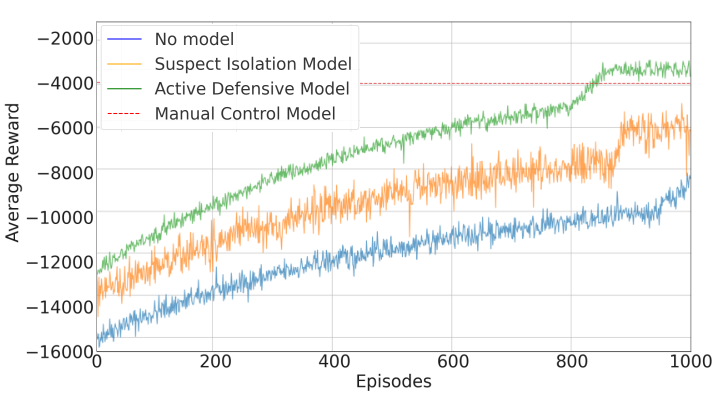
\includegraphics[width=0.9\textwidth]{figures/learning_curves.png}
    \caption{Learning curves for organizational \textit{Manua} in CybORG CAGE Challenge 3.}
    \label{fig:learning_curves}
\end{figure*}

Table \ref{tab:results} summarizes the convergence time, average rewards, and standard deviation achieved by each model during the training process.

\begin{table}[ht]
    \centering
    \scriptsize
    \setlength{\tabcolsep}{3pt}
    \begin{tabular}{|c|c|c|c|}
        \hline
        Model                   & Convergence Time & Average Reward & Standard Deviation \\
        \hline
        No Model                & 115                          & 1.76           & 0.12               \\
        Suspect Isolation Model & 54                           & 1.43           & 0.15               \\
        Greedy Defensive Model  & ?                            & ?              & ?                  \\
        Active Defensive Model  & 80                           & 1.82           & 0.10               \\
        Manual Control Model    & None                         & 1.80           & 0.11               \\
        \hline
    \end{tabular}
    \caption{Performance metrics for organizational models in CybORG CAGE Challenge 3.}
    \label{tab:results}
\end{table}


\subsection{Discussion}

\subsubsection{Qualitative Observations}

The organizational models effectively influenced drone behavior in the CybORG CAGE Challenge 3 environment. The Suspect Isolation Model demonstrated effective identification and isolation of drones exhibiting suspicious activities, enhancing overall security.

\subsubsection{Quantitative Analysis}

{Active Defense Model} showed the highest average reward, indicating its effectiveness in proactive threat mitigation. This model outperformed the Manual Control Model, highlighting the benefits of automated organizational frameworks in dynamic cyber-defense scenarios.

\

The experimental results confirm the importance of organizational models in enhancing coordination and effectiveness among autonomous agents in complex cyber-physical environments like CybORG CAGE Challenge 3.



\section{Conclusion}\label{sec:conclusion}

Our contribution is motivated by addressing the design of a Cyberdefense MAS as an optimization problem under constraints, where the variables to optimize are the agents' policies and the constraints are organizational specifications. This perspective offers two main benefits for tackling the constantly evolving challenges in Cyberdefense: i) It enables the automation/assistance of the design process through MARL techniques, which can be time-consuming and prone to oversight when done manually; ii) It ensures that certain constraints, such as safety guarantees, are satisfied in the agents' behavior, thus aiding in the monitoring and understanding of trained agents.

Building on this idea, we proposed the PRAHOMT algorithm to augment the MARL framework with the $\mathcal{M}OISE^+$ model. PRAHOMT constrains the agents' training according to expected behaviors expressed as organizational specifications. PRAHOMT was evaluated using our proposed PoC implementation for the 3rd CAGE Challenge, a cooperative Cyberdefense drone swarm scenario designed to limit/eliminate malware programs and their impact. We established various organizational models, ranging from minimally constrained to fully constrained ones. We conducted an evaluation of the emergent, fine-tuned, or predefined collective strategies based on performance criteria during and after the training.

The results show that the \textquote{Active Defensive Model} shows a relevant tradeoff between constraints and free learning. It comprises simple predefined rules to detect and mitigate threats when observations clearly indicate them, while allowing the agent to learn how to respond in other situations.

In addition to constraining agents according to organizational specifications, we also aim to integrate explainability mechanisms. Indeed, we intend to characterize and curate relevant emergent strategies to include as new organizational constraints in future training. In this respect, the idea of iterative improvement between training and explainability could greatly benefit from hierarchical learning, which helps better characterize and bring out strategies during learning. Furthermore, while the initial results obtained with LLM show it as a promising complementary tool for PRAHOMT, it may also offer new avenues for explaining collective behavior, especially in Cyberdefense scenarios where most networked environments are not visually or intuitively representable.

% Ultimately, we also aim to improve the applicability of PRAHOM by developing dedicated interfaces built around PRAHOM making it more accessible to industrial and research contexts.



\section*{Acknowledgment}

This work was supported by \emph{Thales Land Air Systems} within the framework of the \emph{Cyb'Air} chair and the \emph{AICA IWG}

\section*{References}

% \bibliographystyle{abbrv}
\bibliographystyle{IEEEtran}

\bibliography{references}

\end{document}
